\documentclass[11pt]{article}
\usepackage{etex}
\reserveinserts{28}
\usepackage{lastpage}
\usepackage[hmargin=2cm, top=2.7cm, bottom=3.5cm, footskip=0.5cm]{geometry}
\usepackage{url}
\usepackage[maxfloats=50]{morefloats}
\usepackage{parskip}
%\usepackage[citestyle=authoryear-comp,natbib=true]{biblatex}
\usepackage{pdflscape}
\usepackage[absolute]{textpos}
\usepackage{rotating} %for xtable sideways
\usepackage{verbatim}
\usepackage{longtable}
\usepackage{multirow}
\usepackage{lipsum}
%\usepackage[acronym,nomain]{glossaries}
\usepackage{fancyhdr, graphicx, lastpage, ifthen, lscape}
\usepackage[dvipsnames, table]{xcolor}
\usepackage{soul}
\usepackage{booktabs}
\usepackage{setspace}
\usepackage{relsize}
\usepackage{tabularx}
\usepackage{makecell}
\usepackage{threeparttable}
\usepackage{threeparttablex}
\usepackage{hyperref}
\usepackage{float}



\bibliography{bibliography.bib}


% For knitr
\usepackage{lmodern}
\usepackage{amssymb,amsmath}
\usepackage{ifxetex,ifluatex}
\usepackage{fixltx2e} % provides \textsubscript
\ifnum 0\ifxetex 1\fi\ifluatex 1\fi=0 % if pdftex
  \usepackage[T1]{fontenc}
  \usepackage[utf8]{inputenc}
\else % if luatex or xelatex
  \ifxetex
    \usepackage{mathspec}
    \usepackage{xltxtra,xunicode}
  \else
    \usepackage{fontspec}
  \fi
  \defaultfontfeatures{Mapping=tex-text,Scale=MatchLowercase}
  \newcommand{\euro}{€}
\fi
% use upquote if available, for straight quotes in verbatim environments
\IfFileExists{upquote.sty}{\usepackage{upquote}}{}
% use microtype if available
\IfFileExists{microtype.sty}{%
\usepackage{microtype}
\UseMicrotypeSet[protrusion]{basicmath} % disable protrusion for tt fonts
}{}
\usepackage{color}
\usepackage{fancyvrb}
\newcommand{\VerbBar}{|}
\newcommand{\B}{\rule[-2ex]{0pt}{0pt}} % bottom strut
\newcommand{\VERB}{\Verb[commandchars=\\\{\}]}
\DefineVerbatimEnvironment{Highlighting}{Verbatim}{commandchars=\\\{\}}
% Add ',fontsize=\small' for more characters per line
\usepackage{framed}
\definecolor{shadecolor}{RGB}{248,248,248}
\newenvironment{Shaded}{\begin{snugshade}}{\end{snugshade}}
\newcommand{\AlertTok}[1]{\textcolor[rgb]{0.94,0.16,0.16}{#1}}
\newcommand{\AnnotationTok}[1]{\textcolor[rgb]{0.56,0.35,0.01}{\textbf{\textit{#1}}}}
\newcommand{\AttributeTok}[1]{\textcolor[rgb]{0.77,0.63,0.00}{#1}}
\newcommand{\BaseNTok}[1]{\textcolor[rgb]{0.00,0.00,0.81}{#1}}
\newcommand{\BuiltInTok}[1]{#1}
\newcommand{\CharTok}[1]{\textcolor[rgb]{0.31,0.60,0.02}{#1}}
\newcommand{\CommentTok}[1]{\textcolor[rgb]{0.56,0.35,0.01}{\textit{#1}}}
\newcommand{\CommentVarTok}[1]{\textcolor[rgb]{0.56,0.35,0.01}{\textbf{\textit{#1}}}}
\newcommand{\ConstantTok}[1]{\textcolor[rgb]{0.00,0.00,0.00}{#1}}
\newcommand{\ControlFlowTok}[1]{\textcolor[rgb]{0.13,0.29,0.53}{\textbf{#1}}}
\newcommand{\DataTypeTok}[1]{\textcolor[rgb]{0.13,0.29,0.53}{#1}}
\newcommand{\DecValTok}[1]{\textcolor[rgb]{0.00,0.00,0.81}{#1}}
\newcommand{\DocumentationTok}[1]{\textcolor[rgb]{0.56,0.35,0.01}{\textbf{\textit{#1}}}}
\newcommand{\ErrorTok}[1]{\textcolor[rgb]{0.64,0.00,0.00}{\textbf{#1}}}
\newcommand{\ExtensionTok}[1]{#1}
\newcommand{\FloatTok}[1]{\textcolor[rgb]{0.00,0.00,0.81}{#1}}
\newcommand{\FunctionTok}[1]{\textcolor[rgb]{0.00,0.00,0.00}{#1}}
\newcommand{\ImportTok}[1]{#1}
\newcommand{\InformationTok}[1]{\textcolor[rgb]{0.56,0.35,0.01}{\textbf{\textit{#1}}}}
\newcommand{\KeywordTok}[1]{\textcolor[rgb]{0.13,0.29,0.53}{\textbf{#1}}}
\newcommand{\NormalTok}[1]{#1}
\newcommand{\OperatorTok}[1]{\textcolor[rgb]{0.81,0.36,0.00}{\textbf{#1}}}
\newcommand{\OtherTok}[1]{\textcolor[rgb]{0.56,0.35,0.01}{#1}}
\newcommand{\PreprocessorTok}[1]{\textcolor[rgb]{0.56,0.35,0.01}{\textit{#1}}}
\newcommand{\RegionMarkerTok}[1]{#1}
\newcommand{\SpecialCharTok}[1]{\textcolor[rgb]{0.00,0.00,0.00}{#1}}
\newcommand{\SpecialStringTok}[1]{\textcolor[rgb]{0.31,0.60,0.02}{#1}}
\newcommand{\StringTok}[1]{\textcolor[rgb]{0.31,0.60,0.02}{#1}}
\newcommand{\VariableTok}[1]{\textcolor[rgb]{0.00,0.00,0.00}{#1}}
\newcommand{\VerbatimStringTok}[1]{\textcolor[rgb]{0.31,0.60,0.02}{#1}}
\newcommand{\WarningTok}[1]{\textcolor[rgb]{0.56,0.35,0.01}{\textbf{\textit{#1}}}}
\providecommand{\tightlist}{%
   \setlength{\itemsep}{0pt}\setlength{\parskip}{0pt}}
\makeatletter
\def\maxwidth{\ifdim\Gin@nat@width>\linewidth\linewidth\else\Gin@nat@width\fi}
\def\maxheight{\ifdim\Gin@nat@height>\textheight\textheight\else\Gin@nat@height\fi}
% End For knitr

\renewcommand{\abstractname}{Overview}

% Add unicode checkmark for DataPackageR support. The green checkmark
% that DataPackageR prints to the console during package_build() causes
% an error with latex. This changes the unicode checkmark to a latex one.
\DeclareUnicodeCharacter{2714}{\checkmark}

% Configure hyperref formatting bookmarks and references
\hypersetup{
  colorlinks = true, % color links instead of covering them w/red boxes
  urlcolor   = blue, % color for external hyperlinks
  linkcolor  = cyan, % color of internal links
  citecolor  = gray  % color of citations
}


%this is to adjust header and footer in landscaped pages
\fancypagestyle{lscape}{%
    \fancyhf{} % clear all header and footer fields
    \fancyhead[R]{\begin{footnotesize}
    \begin{textblock}{1}(0.7,1.5){\color{gray}\rotatebox{90}{ID33-Wilson RSV Correlates Analysis (Version 3.0)}}\end{textblock}
    \end{footnotesize} }
    \fancyfoot[L]{\begin{footnotesize}
    \begin{textblock}{1}(21,1.75){\color{gray}\rotatebox{90}{Page \thepage{}~of~\pageref{LastPage}}}\end{textblock}
    \end{footnotesize} }
    \fancyfoot[R]{\begin{footnotesize}
%     \begin{textblock}{19.8}[-0.01,{\DynLength}](1.5,23.20){\color{gray}\rotatebox{90}{\Rver}}\end{textblock}
    \begin{textblock}{19.8}(1.5,23.20){\color{gray}\rotatebox{90}{\Rver}}\end{textblock}
    \end{footnotesize} }
    \setlength{\TPHorizModule}{1cm}
    \setlength{\TPVertModule}{1cm}
    \renewcommand{\headrulewidth}{0.0pt}
    \renewcommand{\footrulewidth}{0.0pt}}

%set header and footer for first page
\renewcommand{\headrulewidth}{0.8pt}
\renewcommand{\footrulewidth}{0.8pt}
\fancyhead[L]{\includegraphics[height=0.8cm]{C:/Users/bborate/Documents/R/win-library/4.0/VISCtemplates/rmarkdown/templates/visc_report/resources/SCHARP_logo.png}}
\fancyhead[C]{\includegraphics[height=0.8cm]{C:/Users/bborate/Documents/R/win-library/4.0/VISCtemplates/rmarkdown/templates/visc_report/resources/VISC_logo.jpg}}
\fancyhead[R]{\includegraphics[height=0.8cm]{C:/Users/bborate/Documents/R/win-library/4.0/VISCtemplates/rmarkdown/templates/visc_report/resources/FredHutch_logo.png}}
\fancyfoot[C]{Page \thepage{}~of~\pageref{LastPage}}
\setlength{\headheight}{27pt}

%decrease margins for landscape pages
\newenvironment{changemargin}[2]{%
\begin{list}{}{%
\setlength{\topsep}{0pt}%
\setlength{\leftmargin}{#1}%
\setlength{\rightmargin}{#2}%
%\setlength{\listparindent}{\parindent}%
%\setlength{\itemindent}{\parindent}%
\setlength{\parsep}{\parskip}%
}%
\item[]}{\end{list}}

% being able to set emphasis for entire table row
\newcommand\setrow[1]{\gdef\rowmac{#1}#1\ignorespaces}
\newcommand\clearrow{\global\let\rowmac\relax}
\clearrow

%page settings
\setlength{\footskip}{56pt}
\pagestyle{fancy}
\setlength{\parindent}{0pt}
%\makeglossaries
\begin{document}

%get current date into insertdate
\makeatletter
\let\insertdate\@date
\makeatother

% workaround to use landscape environment with pandoc
\newcommand{\blandscape}{\begin{landscape}}
\newcommand{\elandscape}{\end{landscape}}

%begin To and From Section
\makeatletter
\newcommand\tabfill[1]{%
  \dimen@\linewidth
  \advance\dimen@\@totalleftmargin
  \advance\dimen@-\dimen\@curtab
  \parbox[t]\dimen@{%
    \leftskip=2em\hspace*{-2em}#1\ifhmode\strut\fi}%
}
\makeatother

\vspace{0.1cm}
\begin{flushleft}
\begin{tabbing}
this line is to\= set up the tab stop \kill
{\bf Date:} \> \insertdate\\
{\bf To:} \>  \tabfill{Iksung Cho, Matthew Lawlor, Lou Fries}\\
{\bf From:} \> \tabfill{Peter Gilbert, Youyi Fong, Ying Huang, Lars Wim Paul van der Laan, Wenbo Zhang, Bhavesh Borate}\\
{\bf RE:} \> \tabfill{ID33-Wilson RSV Correlates Analysis (Version 3.0)}\\
{\bf cc:} \> \tabfill{Alicia Sato, Eva Chung, Michelle Chung}\\
{\bf Contact:} \> \tabfill{Peter Gilbert, \href{mailto:pgilbert@fredhutch.org}{\nolinkurl{pgilbert@fredhutch.org}} Youyi Fong, \href{mailto:yfong@fredhutch.org}{\nolinkurl{yfong@fredhutch.org}} Ying Huang, \href{mailto:yhuang@fredhutch.org}{\nolinkurl{yhuang@fredhutch.org}}    }\\
\end{tabbing}
\end{flushleft}

\hrule

\vspace{2cm}

%begin contents section
\tableofcontents

%change color of header and footer text to gray
\makeatletter
\patchcmd{\@fancyhead}{\rlap}{\color{gray}\rlap}{}{}
\patchcmd{\headrule}{\hrule}{\color{gray}\hrule}{}{}
\patchcmd{\@fancyfoot}{\rlap}{\color{gray}\rlap}{}{}
\patchcmd{\footrule}{\hrule}{\color{gray}\hrule}{}{}
\makeatother



\listoffigures

\listoftables

\newpage
\fancyhead[R]{\em ID33-Wilson RSV Correlates Analysis (Version 3.0)}
\fancyhead[C]{}
\fancyhead[L]{\em VISC Report}
%\printglossaries

\counterwithin{table}{section}
\counterwithin{figure}{section}
\newcommand{\pathCoRinput}{CoR/input}
\newcommand{\pathThreshinput}{nonparam_threshold/input/y2_Vaccine}
\newcommand{\pathThreshhinput}{nonparam_threshold/input/y1_Vaccine}
\newcommand{\pathThreshpooledinput}{nonparam_threshold/input/y2_Pooled}
\newcommand{\pathThreshhpooledinput}{nonparam_threshold/input/y1_Pooled}

\clearpage

\textbf{Version 2.0 of the RSV immune correlates report} was updated with analyses requested by Dr.~Keith Klugman: Section \protect\hyperlink{posthoc-analysis-to-assess-fold-change-from-maternal-baseline-to-cord-blood-in-immunologic-biomarkers-as-cor-for-endpoint-2}{Posthoc analysis to assess fold change from maternal baseline to cord blood in immunologic biomarkers as CoR for endpoint 2}.

\textbf{Version 3.0 of the RSV immune correlates report} contains enhancements to the non-parametric threshold-risk plots: Figures \ref{fig:PLOT_EIA_log10d14_y1_Vaccine_pointwiseCI}--\ref{fig:PLOT_RSVB_log10cord_y2_Pooled_pointwiseCI} have been revamped with point-wise confidence intervals, superimposed marker-specific reverse CDF (RCDF) plots, and the threshold of no more events has been marked by a vertical red line.

\hypertarget{executive-summary}{%
\section{Executive Summary}\label{executive-summary}}

\hypertarget{approach-to-assessing-immune-correlates-of-risk-and-protection}{%
\subsection{Approach to assessing immune correlates of risk and protection}\label{approach-to-assessing-immune-correlates-of-risk-and-protection}}

The immune correlates analyses were restricted to South African study sites and follow-up period of infants through to 90 days of age.
Correlates for each of three nested RSV disease endpoints in the expanded data set were assessed:
(1) Either RSV LRTI MS, RSV LRTI with hospitalization, or RSV LRTI with severe hypoxemia (52 vaccine and 51 placebo endpoints);
(2) RSV LRTI with severe hypoxemia (14 vaccine and 27 placebo endpoints); and
(3) RSV LRTI with severe hypoxemia without cough (12 vaccine and 26 placebo endpoints). We focus on results for endpoints 1 and 2 given that endpoint 3 was similar to endpoint 2. All analyses were pre-specified in the SAP except one post-hoc analysis that is noted as post-hoc.

Sixteen antibody markers were included in the correlates analyses, as defined by the four assays EIA, PCA, RSVA, RSVB cross-classified by measurement time point and whether fold rise was considered (maternal vaccination sample D0; maternal post vaccination sample D14; maternal fold-rise from D0 to D14; cord blood).
EIA and PCA were measured from all participants, whereas
RSVA and RSVB were measured from all RSV outcome cases and a stratified random sample of non-cases using a two-phase case-control sampling design.

\hypertarget{preliminary-analyses-in-preparation-for-the-correlates-analyses}{%
\subsection{Preliminary analyses in preparation for the correlates analyses}\label{preliminary-analyses-in-preparation-for-the-correlates-analyses}}

Prior to the immune correlates analyses, superlearning was used to develop a maternal enrollment/baseline RSV risk score based on maternal characteristics at enrollment, and to develop an infant birth/delivery RSV risk score based on infant characteristics at birth/delivery. The analysis yielded a maternal enrollment risk score with modest accuracy for predicting whether RSV disease would occur (estimated CV-AUC = 0.56-0.60 depending on endpoint 1 or 2 and vaccine or placebo arm). The most important RSV disease prognostic variables were whether other children \(<\) 5 years of age were in the
home and maternal asthma status.
The infant birth/delivery variables had no ability to predict RSV disease outcome (CV-AUCs \(<\) 0.5). Therefore, all immune correlates analyses adjusted for maternal baseline risk score but not for an infant birth/delivery risk score. In addition, all immune correlates analyses adjusted for the number of days between vaccination and birth.

The D14 EIA and PCA readouts were highly correlated (r = 0.9), yet have different interpretations and thus were both analyzed. The neutralization readouts RSVA and RSVB were moderately correlated with each other (r = 0.5) and with EIA and PCA. The correlation between D0 and D14 readouts in the placebo arm was 0.9 for RSVB/EIA/PCA and 0.7 for RSVA, suggesting that RSVA measurement error was higher than for the other three assays. The correlation between D14 and cord blood readouts in the placebo arm was 0.8 for RSVB/EIA/PCA and 0.7 for RSVA. All four assays were advanced for assessment as immune correlates.

\hypertarget{correlates-of-risk-univariable-markers-objective-to-assess-each-fold-rise-d14-and-cord-blood-marker-as-a-correlate-of-risk-of-rsv-disease}{%
\subsection{Correlates of Risk Univariable Markers: Objective to assess each fold-rise, D14, and cord blood marker as a correlate of risk of RSV disease}\label{correlates-of-risk-univariable-markers-objective-to-assess-each-fold-rise-d14-and-cord-blood-marker-as-a-correlate-of-risk-of-rsv-disease}}

Based on logistic regression modeling, there was no evidence for a correlate of risk of endpoint 1 for any of the markers for either treatment arm
(Figures \ref{hr_forest_y1_trt1} and \ref{hr_forest_y1_trt0}).
In contrast, for endpoint 2, fold-rise of each of the 4 markers RSVA, RSVB, EIA, PCA was inversely associated with outcome,
with estimated odds ratios for the vaccine arm of 0.13, 0.19, 0.19, 0.21 per 10-fold increase of RSVA, RSVB, EIA, and PCA, respectively
(Figure \ref{hr_forest_y2_trt1}). The precision of the correlate was greater for EIA and PCA than for RSVA and RSVB, with narrower confidence intervals about the odds ratios. The result for the fold-rise EIA marker was significant after the pre-specified multiple hypothesis testing adjustment. The message from the results is that for all four assays, fold-rise in vaccine recipients was consistently an inverse correlate of risk of endpoint 2 with a large estimated effect size. Given there were only 14 vaccine breakthrough type 2 endpoints, these consistent results with the 95\% confidence intervals generally lying below one (e.g., 95\% CI 0.06 to 0.62 around the odds ratio estimate of 0.21 for the fold-rise EIA marker) highlights the strong correlations with risk. Point estimates for the D14 versions of the markers, and the cord blood versions of the markers, indicated inverse associations, but with odds ratio estimates closer to one.

Complementing the logistic regression modeling analysis, nonparametric threshold correlates analyses were applied to each D14 and fold-rise antibody marker. Results were reported
as point and simultaneous 95\% confidence interval estimates of the risk of RSV endpoint 1 or 2
varying over subgroups of vaccine recipients defined by antibody marker above a given threshold v, repeating the analysis over all possible thresholds v. The same analyses were done pooling over vaccine and placebo recipients.

For endpoint 1, risk of RSV disease did not vary markedly depending on threshold value of the antibody marker, consistent with the logistic regression results (Figures \ref{fig:PLOT_EIA_log10d14_y1_Vaccine_pointwiseCI}--\ref{fig:PLOT_RSVB_log10cord_y1_Vaccine_pointwiseCI}). In contrast, the results for endpoint 2 showed that for EIA and PCA fold rise, RSV risk sharply decreased across subgroups defined by increasing thresholds, approaching zero risk at highest thresholds (Figures \ref{fig:PLOT_EIA_log10d14overd0_y2_Vaccine_pointwiseCI} and \ref{fig:PLOT_PCA_log10d14overd0_y2_Vaccine_pointwiseCI}). There were no RSV disease endpoint 2 cases above fold-rises of about 20 and 25 for EIA and PCA, respectively. In contrast, RSV risk did not change much across subgroups defined by D14 marker thresholds. RSV risk decreased with threshold of cord blood response, yet with upticks in point estimates in the right tail that rendered the results less clear about potential threshold correlates compared to the fold rise markers. For RSVA and RSVB, there was some decrease in endpoint 2 RSV risk with increasing thresholds of fold-rise, Day 14, and cord blood markers, yet with degree of change less than that for fold rise EIA and fold rise PCA. In conclusion, the threshold analyses supported potential fold rise EIA and PCA threshold correlates for endpoint 2, and did not support threshold correlates for endpoint 1.

\hypertarget{correlates-of-risk-multivariable-markers-objective-to-assess-the-estimated-optimal-surrogate-via-machine-learning-accounting-for-all-of-the-antibody-markers}{%
\subsection{Correlates of Risk Multivariable Markers: Objective to assess the estimated optimal surrogate via machine learning accounting for all of the antibody markers}\label{correlates-of-risk-multivariable-markers-objective-to-assess-the-estimated-optimal-surrogate-via-machine-learning-accounting-for-all-of-the-antibody-markers}}

Superlearning modeling was conducted to build models most predictive of endpoint 1 and to build models most predictive of endpoint 2, within each randomization/treatment arm,
based on each of 29 input variable sets defined by maternal baseline variables and all of the antibody markers measured at D0 and D14 in pregnant mothers and in cord blood in infants. The analyses yielded the following conclusions:

-- Endpoint 1 can be predicted better than endpoint 2, for example for the placebo arm the Superlearner yielded estimated CV-AUC = 0.890 (95\% CI 0.604 to 0.968)
for endpoint 1 (Table \ref{tab:SLperformance-plac-y1}) and estimated CV-AUC = 0.748 (95\% CI 0.577 to 0.862) for endpoint 2
(Table \ref{tab:SLperformance-plac-y2}).

-- RSV disease can be predicted with comparable prediction accuracy in the placebo arm as in the vaccine arm (endpoint 2), or slightly better prediction accuracy in the placebo arm (endpoint 1).

-- The maternal baseline variables alone provided reasonably good classification accuracy, for example estimated CV-AUC = 0.853 (95\% CI 0.636 to 0.948) for endpoint 1 and the placebo arm and estimated CV-AUC = 0.727 (95\% CI 0.548 to 0.851) for endpoint 2 and the placebo arm.

-- Antibody markers improved prediction accuracy compared to only using maternal baseline variables. The best antibody marker predictors were fold-rise EIA and fold-rise PCA, for each endpoint 1 and 2 and each of the vaccine and placebo arms. For example, the Superlearner model for the vaccine arm with EIA fold-rise and maternal baseline variables yielded estimated CV-AUC = 0.859 (95\% CI 0.734 to 0.929) for endpoint 1 (Table \ref{tab:SLperformance-vacc-y1})
and estimated CV-AUC = 0.747 (95\% CI 0.611 to 0.844) for endpoint 2 (Table \ref{tab:SLperformance-vacc-y2}).
D14 markers (not baseline subtracted) were weaker predictors, and RSVA and RSVB markers were inferior predictors to EIA and PCA.

-- Generally the modeling did not support any improved performance gained by including multiple time points or multiple assays/markers in the same predictive model. Fold-rise EIA and fold-rise PCA emerge as the best antibody marker predictors of disease risk as stand-alone markers, providing improved prediction on top of that provided by maternal baseline variables alone. Thus the data support that a single assay/biomarker may provide the best correlate.

\hypertarget{correlates-of-protection-objective-to-assess-immune-cops-as-correlatesmodifiers-of-vaccine-efficacy-against-rsv-disease}{%
\subsection{Correlates of Protection: Objective to assess immune CoPs as correlates/modifiers of vaccine efficacy against RSV disease}\label{correlates-of-protection-objective-to-assess-immune-cops-as-correlatesmodifiers-of-vaccine-efficacy-against-rsv-disease}}

Principal stratification causal inference analyses were conducted to assess how vaccine efficacy (VE) varied over vaccinated subgroups defined by each of four antibody biomarker variables: EIA fold-rise, PCA fold-rise, D14 RSVA, and D14 RSVB. For endpoint 1, the results did not provide evidence that VE was modified by any of the four antibody markers (all p-values \(>\) 0.10). For endpoint 2, the analysis supported that EIA fold-rise was positively correlated with VE against endpoint 2 (p=0.013,
Figure \ref{fig:yingfig1}). For vaccine recipients with fold-rise about 3.2, estimated VE was less than 50\% and the 95\% confidence intervals were wide to the left of this marker value.

The confidence intervals were more precise for larger values of the marker, with estimated VE exceeding 75\% for values of fold-rise above about 16 and approaching 90\% and greater for higher degrees of fold rise. These results support that a 15--20+ fold-rise in EIA is associated with high-level vaccine efficacy. For the other three markers, the results did not provide evidence that VE was modified by any of the antibody markers (all p-values \(>\) 0.10).

\hypertarget{correlates-of-protection-objective-to-assess-immune-cops-in-terms-of-mediators-of-vaccine-efficacy-against-rsv-disease}{%
\subsection{Correlates of Protection: Objective to assess immune CoPs in terms of mediators of vaccine efficacy against RSV disease}\label{correlates-of-protection-objective-to-assess-immune-cops-in-terms-of-mediators-of-vaccine-efficacy-against-rsv-disease}}

We applied formal causal mediation methods to assess each of the four fold-rise and four D14 antibody markers as mediators of VE against endpoint 1 and against endpoint 2. For technical reasons described in the report, the methods did not provide reliable answers. Therefore, we conducted post-hoc exploratory analyses using a standard approach to surrogate endpoint evaluation (Prentice (1989)) that was developed before the formal causal mediation framework was developed. This approach was applied by fitting multiple logistic regression models adjusting for baseline potential confounding variables. Based on this modeling, an antibody marker is supported to meet the Prentice criteria for a valid surrogate endpoint if all of the following conditions are met: (1) there is no evidence of an interaction between randomization arm and the marker; (2) in a main effects model taking out the interaction term, the antibody marker is associated with outcome; (3) in this main effects model, there is no evidence of an association of the treatment/randomization assignment with outcome (i.e., after accounting for the marker, treatment contains no additional information about risk).

The fold rise EIA and PCA markers adhered well to all of the conditions, and thus were supported as potentially valid surrogate endpoints.
In contrast, the fold rise RSVA and RSVB markers failed condition (2), with a significant association of treatment with outcome when the antibody marker was included in the model. This supports that the fold rise EIA and PCA markers have greater validity as surrogate endpoints than the fold rise RSVA and RSVB markers. In addition, all of the D14 markers violated at least one of the conditions (1) through (3).

\hypertarget{overall-conclusions-and-discussion}{%
\subsection{Overall conclusions and discussion}\label{overall-conclusions-and-discussion}}

Fold rise EIA and fold rise PCA (enrollment to D14 post vaccination) had consistent evidence as correlates of risk (CoR) and correlates of protection (CoP) against endpoint 2, based on (1) logistic regression CoR modeling; (2) nonparametric threshold CoR modeling; (3) machine learning multivariable CoR analysis; (4) correlate of VE CoP analysis; and (5) Prentice surrogate endpoint evaluation CoP analysis. Because these two markers were highly correlated, the data support that either marker may be a suitable CoP.

The fold rise markers showed stronger evidence as correlates than the D14 markers. How might this be explained and what are the implications? One hypothesis is that
fold rise is a non-mechanistic CoP where a higher fold rise is a signature of antibody with the right quality to confer protection. Affinity maturation is one putatively important quality, and the association of affinity maturation with fold rise could be tested experimentally.

In theory, a mechanistic CoP would capture the amount of the needed immune response that crossed the placenta and was present during risk of RSV disease during early life. It is possible that fold rise EIA and PCA is better correlated with the amount of antibody present during early life than D14 EIA and PCA. This could be evaluated.

Another question is why were EIA and PCA fold rise better correlates than RSVA and RSVB? The neutralization assays involve three proteins, F, G, and another protein. Only F protein is in the vaccine. The difference in F protein between RSVA and RSVB assay is small, but the G proteins between the two assays may be quite different. The G protein may also drive a large portion of the neutralization responses. On the other hand, EIA and PCA are both F-protein focused. As such, the relevance of the neutralization markers for vaccine protection may have been diminished by the non-F proteins. In addition, the EIA and PCA appeared to have less technical measurement error than the RSVA and RSVB markers, which led to narrower confidence intervals about association parameters based on these markers.

A limitation of the correlates analysis was a small number of evaluable vaccine breakthrough endpoint cases for endpoint 2 (n=14), limiting precision of correlates analyses, and not allowing the formal mediation analyses to be effectively implemented. The fact that strong signals for correlates shone through despite only 14 vaccine breakthrough cases may suggest the strength of fold rise EIA and fold rise PCA as correlates. However, it would be important to seek to replicate the findings or bolster the findings with additional data. One possibility is to seek to validate the correlates using all or a subset of the non-South African sites in the trial.

Another question is why were there no correlates against endpoint 1 and there were correlates against endpoint 2? Both endpoints included RSV LRTI with severe hypoxemia, with difference that endpoint 1 also counted RSV LRTI MS and RSV LRTI with hospitalization as events. This suggests that severe hypoxemia may be the critical aspect of the endpoint that defines a correlate of protection.

\hypertarget{materials-and-methods}{%
\section{Materials and methods}\label{materials-and-methods}}

The materials and methods are fully described in the Statistical Analysis Plan document (Section \protect\hyperlink{statistical-analysis-plan}{Statistical Analysis Plan}). Figure \ref{fig:endpoints_venn_diagrams} shows how the endpoints primarily evaluated for correlates analyses in this report (endpoints 1 and 2) relate to the endpoints defined in the efficacy analyses.

\begin{figure}[H]
    \centering
    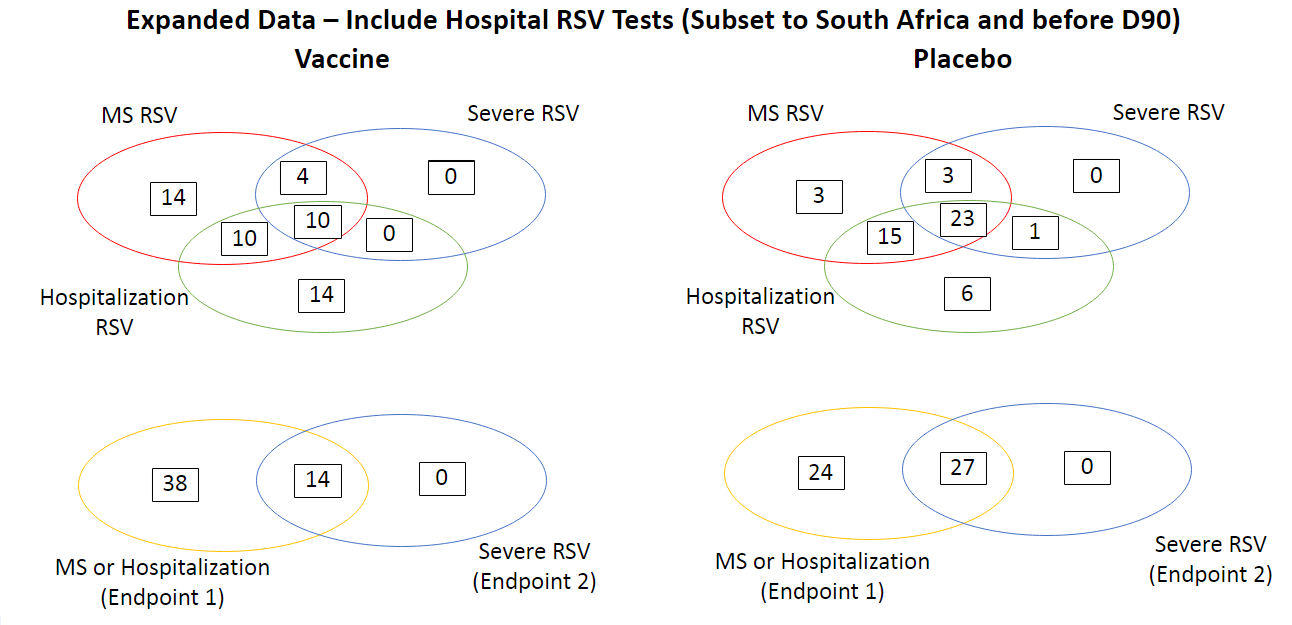
\includegraphics[width=.8\textwidth]{endpoints_venn_diagrams}
    \caption{Venn diagram showing relationship of endpoints 1 and 2 that were evaluated for correlates analyses with endpoints defined in the efficacy analyses. Endpoint 3, RSV LRTI with Severe Hypoxemia without cough, is closely related to and a subset of endpoint 2.}
    \label{fig:endpoints_venn_diagrams}
\end{figure}

\hypertarget{risk-score-analysis}{%
\section{Risk Score analysis}\label{risk-score-analysis}}

\hypertarget{data}{%
\subsection{Data}\label{data}}

The risk score analysis was carried out using data from the placebo group. The two candidate variable sets (maternal enrollment and birth/delivery variable sets) planned for the risk score analysis are shown in Tables \ref{tab:matVarstable} and \ref{tab:pedVarstable} respectively.

\hypertarget{endpoints}{%
\subsection{Endpoints}\label{endpoints}}

Out of the three RSV disease endpoints planned to be studied in the correlates analyses, only two were considered for the risk score analysis, namely:

\begin{enumerate}
\def\labelenumi{\arabic{enumi}.}
\item
  Endpoint 1: {[}``RSV Disease''{]} Composite endpoint defined as the first occurrence of any of the
  three protocol-specified endpoints MS RSV LRTI, RSV LRTI with severe
  hypoxemia, RSV LRTI with hospitalization in the expanded data set, and
\item
  Endpoint 2: RSV LRTI with Severe Hypoxemia
\end{enumerate}

The decision to drop endpoint 3 (RSV LRTI with Severe Hypoxemia without cough) was made on the fact that the total RSV cases based off it were a subset of endpoint 2 with only slightly fewer cases (38 instead of 41) suggesting a minimal impact on the risk score.

\hypertarget{methods}{%
\subsection{Methods}\label{methods}}

The development of the risk score for the maternal enrollment variable set was carried out upon dropping two variables:

\begin{enumerate}
\def\labelenumi{\arabic{enumi}.}
\item
  prebrth variable: had data missing for 349/784 (44\%) of mother-infant pairs, and
\item
  hiv variable: all non-NA values were negative.
\end{enumerate}

Thus, development of the risk score for the maternal variables was based on n=9 covariates. Missing values for covariates were imputed using a multivariable regression method (mice package in R). Except for the child5 covariate, all variables had less than 5\% missing values. Even with a high number of missing values (8.9\%), the child5 variable was included in the analysis as it was found to have a significant association with RSV disease in the placebo group. All covariates were pre-scaled to have a mean of 0 and standard deviation of 1 (including binary, count, and continuous variables).

The development of the risk score for the birth variable set was tried out based on n=8 covariates (Table \ref{tab:pedVarstable}). Two variables, 1) indicator of evidence for GBS colonization, and 2) exposure to intrapartum antibiotic prophylaxis, were not received in data transfer from Novavax. Imputation of missing values and scaling for the covariates in the birth variable set was performed in the same way as for the maternal variable set.

The superlearner ensemble model was based on input from 28 learner-screen combinations shown in Table \ref{tab:learnerScreencombo}. Note that except for the highcor\_random screen, variables passing the screens are further ranked by univariate p-value and the highest ranking variables are selected up to a cap of k variables. Variables passing the highcor\_random screen, in contrast, are selected at random. Thus, the performance of learners with the highcor\_random screen is generally lower in comparison to the other three screens.

Most of the learners used were non-data-adaptive and included glm, glm.interaction, bayesglm, step, lasso (glmnet) and gam. Two data-adaptive learners were also used and included cForest and xgboost.

Two levels of cross-validation (CV) were used in the generation of the superlearner ensemble model:

\begin{enumerate}
\def\labelenumi{\arabic{enumi}.}
\item
  Outer level: CV-AUC is computed over 5-fold CV and used to estimate performance of the ensemble. This is repeated 10 times to improve stability. Note that once the screens are set up, the selected covariates remain constant for the superlearner job (over the 5 outer folds). The variability in the 10 random seeds is generated in the way superlearner splits up the data into the 5 outer folds.
\item
  Inner level: leave-one-out CV used to estimate individual learner performance and ensemble weights.
\end{enumerate}

Eight superlearner models were fit for each endpoint and variable set with model k (among k=1, \ldots, 8) only allowing models with at most k covariates in the model (Table \ref{tab:SLperfriskscore}). The eight superlearner models were compared by CV-AUC and the most parsimonious model (i.e., the model with smallest value of k) with estimated CV-AUC no more than 0.01 less than the superlearner model with highest estimated CV-AUC was selected for each endpoint. Larger models were not considered based on the available sample size.

The selected superlearner models were subsequently used to derive the risk scores defined as the logit of the predicted probability of outcome for each participant. The risk scores for the vaccine recipients were predicted using the selected superlearner models (trained using data from the placebo group). The risk scores for the placebo recipients were derived upon splitting the data into 5 folds. For each of the 5 folds, SL (for the selected k) was trained on the rest of the placebo data and used to predict the probability of outcome. The 5-fold split was repeated 10 times and the probabilities were averaged.

\hypertarget{results}{%
\subsection{Results}\label{results}}

For the maternal enrollment variable set, the best and parsimonious superlearner model selected for endpoint 1 as outcome was for k=1. Performance CV-AUCs of the superlearner and all individual learners for k=1 and endpoint 1 are shown as a forest plot in Figure \ref{fig:riskscoreEndpoint1}. The selected superlearner model had the child5 covariate (indicator for other children \textless{} 5 years of age in home) as a major predictor and gave a CV-AUC of 0.60 for the placebo group and an AUC of 0.59 for the vaccine group. The superlearner model selected for endpoint 2 as outcome was for k=2 (Figure \ref{fig:riskscoreEndpoint2}) and had child5 and maternal asthma status covariates as the major predictors and gave a CV-AUC of 0.60 for the placebo group and an AUC of 0.56 for the vaccine group.
For the birth variable set, no superlearner model was selected as performance CV-AUC with all models was very low (\textless{} 0.5).

Performance CV-AUCs of the superlearner and individual learners for all other k that were not selected to build the risk score are shown in the Appendix section (Figures \ref{fig:riskscoreAppendix1} - \ref{fig:riskscoreAppendix2}).

The two risk scores (one each for endpoint 1 and 2) derived from the maternal enrollment variable set were advanced for use in the immune correlates analyses.

\clearpage

\hypertarget{tables-and-figures}{%
\subsection{Tables and Figures}\label{tables-and-figures}}

\begin{table}[!h]

\caption{\label{tab:maternalVarstable}Maternal enrollment variables. \label{tab:matVarstable}}
\centering
\fontsize{9}{11}\selectfont
\begin{threeparttable}
\begin{tabular}[t]{l>{\raggedright\arraybackslash}p{3cm}l>{\raggedright\arraybackslash}p{3cm}}
\toprule
Variable Name & Definition & Total missing values & Comments\\
\midrule
age.at.trt.cat & Indicator of age > 28 (coded as 1 if age > 28; 0 otherwise) & 0/784 ( 0.0\%) & \\
age.at.trt & Age as continuous variable & 0/784 ( 0.0\%) & \\
bmi & BMI & 1/784 ( 0.1\%) & \\
mhsmopr & Smoker status & 0/784 ( 0.0\%) & \\
m.ast & Asthma status & 0/784 ( 0.0\%) & \\
child5 & Indicator other children < 5 years of age in home & 70/784 ( 8.9\%) & \\
season & RSV season intensity score at time of birth & 0/784 ( 0.0\%) & \\
smoker & Indicator of infant living with smoker & 2/784 ( 0.3\%) & \\
daycare & Indicator of daycare, or infant living in home with daycare attendee & 3/784 ( 0.4\%) & \\
prebrth & Number of previous children & 349/784 (44.5\%) & dropped from analysis\\
hiv & HIV & 4/784 ( 0.5\%) & all non-NA values are negative; dropped from analysis\\
\bottomrule
\end{tabular}
\begin{tablenotes}
\item \textit{Note: } 
\item Missing values for variables not dropped from analysis were imputed.
\end{tablenotes}
\end{threeparttable}
\end{table}

\begin{table}[!h]

\caption{\label{tab:pedVars}Delivery/Birth variables. \label{tab:pedVarstable}}
\centering
\fontsize{9}{11}\selectfont
\begin{threeparttable}
\begin{tabular}[t]{l>{\raggedright\arraybackslash}p{3cm}l>{\raggedright\arraybackslash}p{3cm}}
\toprule
Variable Name & Definition & Total missing values & Comments\\
\midrule
p.sex & Infant gender & 0/784 (0.0\%) & \\
iwt & Birthweight (continuous) & 3/784 (0.4\%) & \\
p.lbw & Birthweight (low vs. not low) & 0/784 (0.0\%) & \\
iwtlen & Ratio of length to birthweight & 23/784 (2.9\%) & \\
hdcirc & Frontal occipital head circumference & 7/784 (0.9\%) & \\
ga & Estimated gestational age at birth in days (count variable) & 6/784 (0.8\%) & \\
p.small & Small for gestational age & 0/784 (0.0\%) & \\
p.igr & Intrauterine growth retardation & 0/784 (0.0\%) & \\
\bottomrule
\end{tabular}
\begin{tablenotes}
\item \textit{Note: } 
\item Two birth variables, 1) indicator of evidence for GBS colonization, and 2) exposure to intrapartum antibiotic prophylaxis, were not received in data transfer from Novavax.
\item Missing values for variables not dropped from analysis were imputed.
\end{tablenotes}
\end{threeparttable}
\end{table}

\begin{table}[!h]

\caption{\label{tab:learner-screens}All learner-screen combinations (28 in total) used as input to the superlearner. The k parameter allows models
with at most k covariates and is appended at the end of the screen name. k ranges from 1:8 for both the maternal enrollment and birth/delivery variable sets. \label{tab:learnerScreencombo}}
\centering
\fontsize{9}{11}\selectfont
\begin{threeparttable}
\begin{tabular}[t]{>{\raggedright\arraybackslash}p{5cm}>{\raggedright\arraybackslash}p{5cm}}
\toprule
\textbf{Learner} & \textbf{Screen*}\\
\midrule
SL.mean & all\_k\\
\cmidrule{1-2}
 & all\_k\\

 & glmnet\_k\\

 & univar\_logistic\_pval\_k\\

\multirow[t]{-4}{5cm}{\raggedright\arraybackslash SL.glm} & highcor\_random\_k\\
\cmidrule{1-2}
 & all\_k\\

 & glmnet\_k\\

 & univar\_logistic\_pval\_k\\

\multirow[t]{-4}{5cm}{\raggedright\arraybackslash SL.glm.interaction} & highcor\_random\_k\\
\cmidrule{1-2}
 & all\_k\\

 & glmnet\_k\\

 & univar\_logistic\_pval\_k\\

\multirow[t]{-4}{5cm}{\raggedright\arraybackslash SL.bayesglm} & highcor\_random\_k\\
\cmidrule{1-2}
 & glmnet\_k\\

 & univar\_logistic\_pval\_k\\

\multirow[t]{-3}{5cm}{\raggedright\arraybackslash SL.step} & highcor\_random\_k\\
\cmidrule{1-2}
 & glmnet\_k\\

 & univar\_logistic\_pval\_k\\

\multirow[t]{-3}{5cm}{\raggedright\arraybackslash SL.glmnet} & highcor\_random\_k\\
\cmidrule{1-2}
 & glmnet\_k\\

 & univar\_logistic\_pval\_k\\

\multirow[t]{-3}{5cm}{\raggedright\arraybackslash SL.gam} & highcor\_random\_k\\
\cmidrule{1-2}
 & glmnet\_k\\

 & univar\_logistic\_pval\_k\\

\multirow[t]{-3}{5cm}{\raggedright\arraybackslash SL.cforest} & highcor\_random\_k\\
\cmidrule{1-2}
 & glmnet\_k\\

 & univar\_logistic\_pval\_k\\

\multirow[t]{-3}{5cm}{\raggedright\arraybackslash SL.xgboost} & highcor\_random\_k\\
\bottomrule
\end{tabular}
\begin{tablenotes}
\item \textit{Note: } 
\item *Screen details:
\item all\_k: includes all variables
\item glmnet\_k: includes variables with non-zero coefficients in the standard implementation of SL.glmnet that optimizes the lasso tuning parameter via cross-validation
\item univar\_logistic\_pval\_k: Wald test 2-sided p-value in a logistic regression model < 0.10
\item highcor\_random\_k: if pairs of quantitative variables with Spearman rank correlation > 0.90, select one of the variables at random
\end{tablenotes}
\end{threeparttable}
\end{table}

\clearpage

\begin{table}[!h]

\caption{\label{tab:riskscore-SLperformance}Superlearner performance (CV-AUCs) for each k, variable set, and endpoint. The k parameter allows models
with at most k covariates. k ranges from 1:8 for both maternal enrollment and birth/delivery variable sets. \label{tab:SLperfriskscore}}
\centering
\fontsize{7}{9}\selectfont
\begin{tabular}[t]{l>{\raggedright\arraybackslash}p{3.5cm}>{\raggedright\arraybackslash}p{3.5cm}>{\raggedright\arraybackslash}p{3.0cm}>{\raggedright\arraybackslash}p{3.0cm}}
\toprule
k & maternal vars: endpoint 1 & maternal vars: endpoint 2 & birth vars: endpoint 1 & birth vars: endpoint 2\\
\midrule
1 & 0.604 [0.586, 0.623] & 0.553 [0.526, 0.579] & 0.479 [0.459, 0.499] & 0.457 [0.435, 0.478]\\
2 & 0.596 [0.580, 0.612] & 0.600 [0.578, 0.621] & 0.477 [0.461, 0.493] & 0.460 [0.442, 0.478]\\
3 & 0.581 [0.567, 0.596] & 0.584 [0.565, 0.604] & 0.484 [0.468, 0.501] & 0.479 [0.460, 0.498]\\
4 & 0.599 [0.585, 0.613] & 0.581 [0.562, 0.600] & 0.468 [0.451, 0.485] & 0.479 [0.459, 0.500]\\
5 & 0.597 [0.584, 0.611] & 0.545 [0.526, 0.563] & 0.473 [0.455, 0.491] & 0.482 [0.463, 0.502]\\
6 & 0.595 [0.581, 0.609] & 0.574 [0.556, 0.592] & 0.454 [0.438, 0.470] & 0.468 [0.447, 0.488]\\
7 & 0.595 [0.581, 0.609] & 0.574 [0.556, 0.592] & 0.462 [0.445, 0.479] & 0.470 [0.449, 0.490]\\
8 & 0.591 [0.578, 0.605] & 0.590 [0.573, 0.608] & 0.467 [0.449, 0.485] & 0.470 [0.450, 0.490]\\
\bottomrule
\end{tabular}
\end{table}

\hypertarget{most-parsimonious-lowest-k-superlearner-models-with-optimal-cv-auc-selected-to-derive-the-risk-score}{%
\subsection{Most parsimonious (lowest k) superlearner models with optimal CV-AUC selected to derive the risk score}\label{most-parsimonious-lowest-k-superlearner-models-with-optimal-cv-auc-selected-to-derive-the-risk-score}}

\hypertarget{maternal-enrollment-variable-set}{%
\subsubsection{Maternal enrollment variable set}\label{maternal-enrollment-variable-set}}

\begin{figure}[H]

{\centering \includegraphics[width=1\linewidth,]{C:/figure-latex/SL-fits-mat1-y1-1} 

}

\caption[Risk score analysis for maternal enrollment variables with k=1 and endpoint 1.]{\label{fig:riskscoreEndpoint1}Risk score analysis for maternal enrollment variables with k=1 and endpoint 1: Plot shows CV-AUC point estimates and 95\% confidence intervals for the Super Learner and all models trained to classify RSV cases in the placebo group defined by endpoint 1. Learners are sorted by their CV-AUC point estimates.}\label{fig:SL-fits-mat1-y1}
\end{figure}

\begin{figure}[H]

{\centering \includegraphics[width=1\linewidth,]{C:/figure-latex/SL-fits-mat2-y2-1} 

}

\caption[Risk score analysis for maternal enrollment variables with k=2 and endpoint 2.]{\label{fig:riskscoreEndpoint2}Risk score analysis for maternal enrollment variables with k=2 and endpoint 2: Plot shows CV-AUC point estimates and 95\% confidence intervals for the Super Learner and all models trained to classify RSV cases in the placebo group defined by endpoint 2. Learners are sorted by their CV-AUC point estimates.}\label{fig:SL-fits-mat2-y2}
\end{figure}

\clearpage

\hypertarget{immune-biomarkers-unsupervised-exploratory-analysis-preparation-for-correlates-analyses}{%
\section{Immune biomarkers unsupervised exploratory analysis (preparation for correlates analyses)}\label{immune-biomarkers-unsupervised-exploratory-analysis-preparation-for-correlates-analyses}}

\hypertarget{comparion-between-time-points}{%
\subsection{Comparion between time points}\label{comparion-between-time-points}}

In the vaccine arm there is a drop from d14 to cord blood for all four markers.
In the placebo arm there is a small drop from d14 to cord blood in RSVA, but this is not observed for RSVB, EIA, or PCA.

\begin{figure}[H]
    \centering
    \includegraphics[width=1\textwidth]{exploratory/input/boxplot_rsv_by_time_trt.png}
    \caption{Boxplots of RSVA and RSVB}
\end{figure}

\begin{figure}[H]
    \centering
    \includegraphics[width=1\textwidth]{exploratory/input/boxplot_eia_pca_by_time_trt.png}
    \caption{Boxplots of EIA and PCA}
\end{figure}

\clearpage

\hypertarget{correlations-between-assays}{%
\subsection{Correlations between assays}\label{correlations-between-assays}}

The correlations between EIA and PCA are high (around 0.9), especially in the vaccine arm at the D14 and cord blood time points. The correlations between RSVA and other assays and the correlations between RSVB and other assays are moderate (around 0.5); therefore, according to the SAP we advance both markers to the correlates analyses.

\begin{table}[H]
    \centering
    \input{exploratory/input/spearcor_assays}
    \caption{Average of Spearman correlation coefficients between assays at different times and in different treatment arms.}
\end{table}

A potential explanation for the relatively low correlations between RSVA and other assays and between RSVB and other assays is that neutralization assays involve three proteins, F, G, and another protein. Only F protein is in the vaccine. The difference in F protein between RSVA and RSVB assay is not very big, but the G proteins between the two assays may be quite different. The G protein may also drive a large portion of the neutralization responses. On the other hand, EIA and PCA are both F-protein focused.

Much of the titer data are not as discrete as the RSVA and RSVB data. EIA is based on titer data (although the documentation from Novavax is ambiguous on this, in some places it says the readout is OD), if all it takes is to fit 4PL and smooth it out, that should be easy to do.
There were no replicates for RSVA and RSVB markers, which made it hard to assess assay variability and we are left wondering whether the relatively poor performance of RSVA and RSVB is due to assay variability or to other explanations such as the one Lou discussed: F protein in the vaccine may not be the dominant factor for this assay. Understandably the lack of replicates is due to cost, but the lab should have some data on the assay variability from their quality control process.
The correlation between D0 and D14 in the placebo arm provides an estimate of the measurement error. The correlation is high, around 0.9, for RSVB, EIA, and PCA, but lower, around 0.7, for RSVA.

\begin{figure}[!ht]
    \centering
    \includegraphics[width=1\textwidth]{exploratory/input/scatterplot_rsva_rsvb.pdf}
    \caption{Scatterplots between RSV A and B by treatment and time. Spearman correlation coefficients are shown in the titles.}
\end{figure}

\begin{figure}[!ht]
    \centering
    \includegraphics[width=1\textwidth]{exploratory/input/scatterplot_eia_pca.pdf}
    \caption{Scatterplots between EIA and PCA by treatment and time. Spearman correlation coefficients are shown in the titles.}
    \label{fig:scatterplot_eia_pca}
\end{figure}

\begin{figure}[!ht]
    \centering
    \includegraphics[width=1\textwidth]{exploratory/input/scatterplot_rsva_eia.pdf}
    \caption{Scatterplots between RSV A and EIA by treatment and time. Spearman correlation coefficients are shown in the titles.}
\end{figure}

\begin{figure}[!ht]
    \centering
    \includegraphics[width=1\textwidth]{exploratory/input/scatterplot_rsva_pca.pdf}
    \caption{Scatterplots between RSV A and PCA by treatment and time. Spearman correlation coefficients are shown in the titles.}
\end{figure}

\clearpage

\hypertarget{correlations-between-time-points}{%
\subsection{Correlations between time points}\label{correlations-between-time-points}}

In this subsection we examine correlations between assay measurements at different time points.

\begin{table}[H]
    \centering
    \input{exploratory/input/spearcor_time_d14}
    \caption{Spearman correlation coefficients between D0 and D14.}
\end{table}

\begin{table}[H]
    \centering
    \input{exploratory/input/spearcor_time_foldchange}
    \caption{Spearman correlation coefficients between D0 and fold-change (D14 over D0)}
\end{table}

\clearpage
\begin{figure}[H]
    \centering
    \includegraphics[width=1\textwidth]{exploratory/input/scatterplot_RSVA.pdf}
    \caption{RSV A. Spearman correlation coefficients are shown in the titles.}
    \label{fig:scatterplot_RSVA}
\end{figure}

\begin{figure}[H]
    \centering
    \includegraphics[width=1\textwidth]{exploratory/input/scatterplot_RSVB.pdf}
    \caption{RSV B. Spearman correlation coefficients are shown in the titles.}
    \label{fig:scatterplot_RSVB}
\end{figure}

\begin{figure}[H]
    \centering
    \includegraphics[width=1\textwidth]{exploratory/input/scatterplot_EIA.pdf}
    \caption{EIA. Spearman correlation coefficients are shown in the titles.}
    \label{fig:scatterplot_EIA}
\end{figure}

\begin{figure}[H]
    \centering
    \includegraphics[width=1\textwidth]{exploratory/input/scatterplot_PCA.pdf}
    \caption{PCA. Spearman correlation coefficients are shown in the titles.}
    \label{fig:scatterplot_PCA}
\end{figure}

\begin{figure}[H]
    \centering
    \includegraphics[width=1\textwidth]{exploratory/input/scatterplot_rsvAB_d14_foldchange}
    \caption{RSVA and RSVB.}
\end{figure}

\begin{figure}[H]
    \centering
    \includegraphics[width=1\textwidth]{exploratory/input/scatterplot_EIApca_d14_foldchange}
    \label{fig:scatterplot_EIApca_d14_foldchange}
    \caption{EIA and PCA. The top 4 data points in EIA placebo arm are best in both D14 values and fold change. If these are new infections, then the attack rate is about 1.5\% annually, which is within range. }
\end{figure}

\clearpage

\clearpage

\hypertarget{correlates-of-risk}{%
\section{Correlates of risk}\label{correlates-of-risk}}

\hypertarget{correlates-of-risk-objective-1}{%
\subsection{Correlates of risk objective 1}\label{correlates-of-risk-objective-1}}

In this objective we assessed the association of each of the 16 immunologic biomarkers, one-at-a-time, with each of the three endpoints within each study arm. All markers were on the log10 scale.

For maternal time points (D0, D14), the analyses adjusted for the maternal risk score and the indicator for whether the number of days from vaccination to birth was greater than or equal to 30 days; for cord blood markers, the analyses adjusted for the maternal risk score alone.

Results for EIA and PCA were estimated from phase 1 data using the glm function.
Results for RSVA and RSVB were estimated from phase 2 data using the osDesign package (Breslow and Holubkov (1997)) for endpoint 1 and the survey package (Lumley (2010)) for endpoints 2 and 3.
\bigskip

osDesign was the specified regression method in the SAP. In the terminology used by osDesign, there were 20 strata in our design, 10 in vaccine and 10 in placebo (crossing 5 regions with time from vaccination to birth less than 30 days (\textless30d)). The numbers of cases and controls in these strata were input to osDesign::tps; no counts can be zero, otherwise we obtained a ``zero cell frequency at phase I'' error. For endpoint 1, there were no cases in the stratum SS/\textless30d in both the placebo arm and the vaccine arm. These two had small strata: 11 controls in the placebo arm (out of 784 total) and 18 controls in the vaccine arm (out of 1553 total) and 2 controls from each stratum were sampled for biomarkers measurements. We thus removed these two strata from the analyses for endpoint 1.
\bigskip

An alternative method for making inference based on phase 2 data is to use the svyglm function from the survey package. Results for RSVA and RSVB for endpoint 1 using the survey package (not shown) were close to the results obtained using the osDesign package. For endpoints 2 and 3, four out of ten strata in placebo and five out of ten strata in vaccine are empty, so we used the survey package for endpoints 2 and 3. For the survey package, when a stratum has only one sample, ``there is no contribution to the variance from the first stage of sampling in this stratum,'' (\url{https://r-survey.r-forge.r-project.org/survey/exmample-lonely.html}), the survey package offers several options, and the best option to us seems to be options(survey.lonely.psu=``adjust''), by which ``the stratum contribution to the variance is taken to be the average of all the strata with more than one primary sampling unit. This might be appropriate if the lonely PSUs were due to data missing at random rather than to design deficiencies. Other options include removing the strata or ignore the first stage sampling variance in those strata.''
\bigskip

Based on logistic regression modeling, there was no evidence for a correlate of risk of endpoint 1 for any of the markers for either treatment arm
(Figures \ref{hr_forest_y1_trt1} and \ref{hr_forest_y1_trt0}).
In contrast, for endpoint 2, fold-rise of each of the 4 markers EIA, PCA, RSVA, RSVB was inversely associated with outcome,
with odds ratios for the vaccine arm of 0.13, 0.19, 0.19, 0.21 per 10-fold increase of RSVA, RSVB, EIA, and PCA, respectively
(Figure \ref{hr_forest_y2_trt1}). The precision of the correlate was greater for EIA and PCA than for RSVA and RSVB, with narrower confidence intervals about the odds ratios. Figure
\ref{hr_forest_y2_trt0} shows results for endpoint 2 and the placebo arm.

For CoR objective 1, the only marker that passed the preset criterion of either q value of 0.1 or the more stringent Holm-adjusted p value of 0.05 was EIA fold change (d14 over d0) for endpoint 2 in the vaccine arm, which had a P value of 0.005 and q value of 0.085 (Table \ref{tab:CoR_obj1a_pvals}). In fact, Table \ref{tab:CoR_obj1a} shows that not just EIA, but also PCA and RSVB fold change, have an inverse association with risk for endpoint 2 in the vaccine arm that was significant before multiplicity adjustment, and RSVA also has a trend. The point and 95\% confidence interval estimates of odds ratios support substantial inverse associations of each antibody marker with RSV risk. Therefore, the message from the results is that for all four assays, fold-rise in vaccine recipients was consistently an inverse correlate of risk of endpoint 2 with a large estimated effect size. Given there were only 14 vaccine breakthrough type 2 endpoints, these consistent results with the 95\% confidence intervals generally lying below one (e.g., 95\% CI 0.06 to 0.62 around the odds ratio estimate of 0.21 for the fold-rise EIA marker) highlights the strong correlates effect sizes. Point estimates for the D14 versions of the markers, and the cord blood versions of the markers, indicated inverse associations, but with odds ratio estimates much closer to one.

\bigskip

In the placebo arm, the log10 d0 measurements for the four assays showed no association with outcome. In the vaccine arm, the log10 d0 measurements showed trends toward direct associations with RSV risk; this can be explained as an induced association because d0 measurement is inversely associated with fold change. (When we include both d0 and fold change EIA in the same model for endpoint 2 and the vaccine arm, both are inversely correlated with risk. But to see the effect of fold change, we should not adjust for baseline, because baseline is associated with fold change. Leaving baseline out is justified because in the placebo arm it is not associated with risk.)
\bigskip

EIA or PCA were fitted using phase 2 data in order to compare with RSVA and RSVB to see which ones appeared to be stronger correlates on a more fair footing. The results suggest that EIA was better than RSVA and RSVB, which in turn were better than PCA. It is interesting that EIA and PCA were highly correlated (Pearson 0.95 in phase 2) and yet their performances as correlates of risk differed.
\bigskip

For endpoint 2 and the vaccine arm, the single marker regression p value for EIA fold change was 0.00627; the multiplicity Holm and BH adjusted p values were 0.100 and 0.100.
The multiplicity adjustment approach we took may have been conservative because it did not account for the correlation between markers, and all markers were included in the multiplicity adjustment. Alternative less-conservative approaches to multiplicity adjustment would be the following:

\begin{enumerate}
\def\labelenumi{\arabic{enumi})}
\tightlist
\item
  Due to correlation between markers, a permutation-based procedure may be worth doing.
\item
  We could be more selective in which markers to include in the multiplicity adjustment. For example, we may exclude cord blood markers, baseline markers, or both from multiplicity adjustment and treat them as secondary objectives.
\end{enumerate}

Some post-hoc exploratory preliminary Westfall and Young permutation-based multiplicity adjusted p values (Westfall and Young (1989)) for endpoint 2 and the vaccine arm are shown in Table \ref{tab:CoR_obj1a_y2_trt1_padj}. The permutation procedure can be potentially improved because the fact that we have a mix of phase 1 and phase 2 analyses presents a challenge. Furthermore, p.FWER is 0.0443 if cord blood is dropped, and 0.0311 if cord blood and baseline are dropped. These results are preliminary because the way permutation is done is complicated by the fact that some markers are phase 1 and some are phase 2. In these results, these facts were ignored when permuting and fit glm for all markers.

\clearpage
\begin{table}[H]
\tiny{
    \textbf{Endpoint 1}\\
    Vaccine arm\\
    \input{CoR/input/CoR_obj1a_y1_trt1}
    
    % it is important to have this empty line above for formatting
    \vspace{5pt}
    Placebo arm\\
    \input{CoR/input/CoR_obj1a_y1_trt0}

    \bigskip
    \textbf{Endpoint 2}\\
    Vaccine arm\\
    \input{CoR/input/CoR_obj1a_y2_trt1}
    
    \vspace{5pt}
    Placebo arm\\
    \input{CoR/input/CoR_obj1a_y2_trt0}

    \bigskip
    \textbf{Endpoint 3}\\
    Vaccine arm\\
    \input{CoR/input/CoR_obj1a_y3_trt1}
    
    \vspace{5pt}
    Placebo arm\\
    \input{CoR/input/CoR_obj1a_y3_trt0}
}
    \caption{CoR objective 1. Each cell corresponds to one model. RSVA and RSVB models are fitted to phase 2 data, PCA and EIA models are fitted to phase 1 data.
    Time from vaccination to birth is adjusted for in analyses of maternal markers but not in analyses of infant markers. All models adjust for maternal risk score.
     Phase 1 data are used for EIA and PCA.
     }
    \label{tab:CoR_obj1a}
\end{table}

\clearpage
\begin{table}[H]
\scriptsize{
    \textbf{Endpoint 1}\\
    \input{CoR/input/CoR_obj1a_y1_trt1_pvals}    
    \quad
    \input{CoR/input/CoR_obj1a_y1_trt0_pvals}

    \bigskip
    \textbf{Endpoint 2}\\
    \input{CoR/input/CoR_obj1a_y2_trt1_pvals}    
    \quad
    \input{CoR/input/CoR_obj1a_y2_trt0_pvals}

    \bigskip
    \textbf{Endpoint 3}\\
    \input{CoR/input/CoR_obj1a_y3_trt1_pvals}    
    \quad
    \input{CoR/input/CoR_obj1a_y3_trt0_pvals}
}
    \caption{P-values multiplicity adjustment for CoR objective 1. Vaccine arm on the left and placebo arm on the right. Phase 1 data are used for EIA and PCA.}
    \label{tab:CoR_obj1a_pvals}
\end{table}

\clearpage
\begin{table}[H]
    \input{CoR/input/CoR_obj1a_y2_trt1_padj}
    \caption{CoR objective 1, endpoint 2, vaccine arm. Westfall and Young permutation-based multiplicity adjustment. Permutation is done by tethering the end point and the clinical covariates together and permuting the marker only. 
     }
    \label{tab:CoR_obj1a_y2_trt1_padj}
\end{table}

\clearpage
\begin{table}[H]
\tiny{
    \textbf{Endpoint 1}\\
    Vaccine arm\\
    \input{CoR/input/CoR_obj1b_y1_trt1}
    
    % it is important to have this empty line above for formatting
    \vspace{5pt}
    Placebo arm\\
    \input{CoR/input/CoR_obj1b_y1_trt0}

    \bigskip
    \textbf{Endpoint 2}\\
    Vaccine arm\\
    \input{CoR/input/CoR_obj1b_y2_trt1}
    
    \vspace{5pt}
    Placebo arm\\
    \input{CoR/input/CoR_obj1b_y2_trt0}

    \bigskip
    \textbf{Endpoint 3}\\
    Vaccine arm\\
    \input{CoR/input/CoR_obj1b_y3_trt1}
    
    \vspace{5pt}
    Placebo arm\\
    \input{CoR/input/CoR_obj1b_y3_trt0}
}
    \caption{CoR objective 1. Each cell corresponds to one model. All marker models are fitted to phase 2 data. Time from vaccination to birth is adjusted for in analyses of maternal markers but not in analyses of infant markers. All models adjust for maternal risk score.
     Phase 2 data are used for EIA and PCA.}
    \label{tab:CoR_obj1b}
\end{table}

\clearpage
\begin{table}[H]
\scriptsize{
    \textbf{Endpoint 1}\\
    \input{CoR/input/CoR_obj1b_y1_trt1_pvals}    
    \quad
    \input{CoR/input/CoR_obj1b_y1_trt0_pvals}

    \bigskip
    \textbf{Endpoint 2}\\
    \input{CoR/input/CoR_obj1b_y2_trt1_pvals}    
    \quad
    \input{CoR/input/CoR_obj1b_y2_trt0_pvals}

    \bigskip
    \textbf{Endpoint 3}\\
    \input{CoR/input/CoR_obj1b_y3_trt1_pvals}    
    \quad
    \input{CoR/input/CoR_obj1b_y3_trt0_pvals}
}
    \caption{P-values multiplicity adjustment for CoR objective 1. Vaccine arm on the left and placebo arm on the right.  Phase 2 data are used for EIA and PCA.}
    \label{tab:CoR_obj1b_pvals}
\end{table}

\begin{figure}[H]
    \centering
    \includegraphics[width=\textwidth]{CoR/input/../../exploratory/input/boxplot_log10d14overd0_by_y1_vacc}
    \caption{Boxplots of fold change (D14 over D0) by endpoint 1 status in the vaccine arm}
    \label{fig:boxplot_log10d14overd0_by_y1_vacc}
\end{figure}

\begin{figure}[H]
    \centering
    \includegraphics[width=\textwidth]{CoR/input/../../exploratory/input/boxplot_log10d14overd0_by_y2_vacc}
    \caption{Boxplots of fold change (D14 over D0) by endpoint 2 status in the vaccine arm}
    \label{fig:boxplot_log10d14overd0_by_y2_vacc}
\end{figure}

\begin{figure}[H]
    \centering
    \includegraphics[width=\textwidth]{CoR/input/../../exploratory/input/boxplot_log10d14overd0_by_y3_vacc}
    \caption{Boxplots of fold change (D14 over D0) by endpoint 3 status in the vaccine arm}
    \label{fig:boxplot_log10d14overd0_by_y3_vacc}
\end{figure}

\clearpage

\begin{figure}[H]
    \centering
    \includegraphics[width=.3\textwidth]{CoR/input/marginal_risk_EIA.log10d14overd0}
    \includegraphics[width=.3\textwidth]{CoR/input/marginal_risk_EIA.log10d14overd0_adjd0}
    \includegraphics[width=.3\textwidth]{CoR/input/marginal_risk_EIA}
    \caption{Marginalized risk plots in the vaccine arm. These plots are based on the risk regression model, averaging over the distribution of maternal risk score and number of days between vaccination and birth. The horizontal lines indicate the overall risk in the placebo arm. 95\% bootstrap confidence bands are shown. Left: not adjusted for baseline concentration; middle: showing both adjusted and not adjusted for baseline concentration; right: comparing D14 and fold rise (not adjusted for baseline concentration).}
    \label{fig:marginal_risk_EIA.log10d14overd0}
\end{figure}

\clearpage
\begin{figure}[H]
    \centering
    \includegraphics[width=1\textwidth]{CoR/input/hr_forest_y1_trt1}
    \caption{Forest plots of odds ratios of Day 14 and fold rise markers for endpoint 1 in the vaccine arm.}
    \label{hr_forest_y1_trt1}
\end{figure}
\begin{figure}[H]
    \centering
    \includegraphics[width=1\textwidth]{CoR/input/hr_forest_y1_trt0}
    \caption{Forest plots of odds ratios of Day 14 and fold rise markers for endpoint 1 in the placebo arm.}
    \label{hr_forest_y1_trt0}
\end{figure}
\clearpage

\begin{figure}[H]
    \centering
    \includegraphics[width=1\textwidth]{CoR/input/hr_forest_y2_trt1}
    \caption{Forest plots of odds ratios of Day 14 and fold rise markers for endpoint 2 in the vaccine arm.}
    \label{hr_forest_y2_trt1}
\end{figure}
\begin{figure}[H]
    \centering
    \includegraphics[width=1\textwidth]{CoR/input/hr_forest_y2_trt0}
    \caption{Forest plots of odds ratios of Day 14 and fold rise markers for endpoint 2 in the placebo arm.}
    \label{hr_forest_y2_trt0}
\end{figure}
\clearpage

\begin{figure}[H]
    \centering
    \includegraphics[width=1\textwidth]{CoR/input/hr_forest_y3_trt1}
    \caption{Forest plots of odds ratios of Day 14 and fold rise markers for endpoint 3 in the vaccine arm.}
    \label{hr_forest_y3_trt1}
\end{figure}
\begin{figure}[H]
    \centering
    \includegraphics[width=1\textwidth]{CoR/input/hr_forest_y3_trt0}
    \caption{Forest plots of odds ratios of Day 14 and fold rise markers for endpoint 3 in the placebo arm.}
    \label{hr_forest_y3_trt0}
\end{figure}
\clearpage

The van der Laan, Zhang, and Gilbert (2020) extension of the nonparametric CoR threshold estimation method of Donovan, Hudgens, and Gilbert (2019) was applied to each D14, fold-rise, and cord blood antibody marker. This extension adjusts for the baseline covariates maternal baseline risk score and the number of days between vaccination and birth using targeted maximum likelihood estimation (TMLE). Results are reported as plots of point and simultaneous 95\% confidence interval estimates of the risk of RSV endpoint 1 or 2 varying over subgroups of vaccine recipients defined by antibody marker above a given threshold v, and repeating the analysis over all possible thresholds v. The same analysis was done pooling over vaccine and placebo recipients.

The following subsections show results for the vaccine arm and pooled (vaccine + placebo arm) arms for each of the four antibody markers, as fold-rise, D14 values, and cord blood values, and for endpoint 1 and endpoint 2. For endpoint 1, the results show that risk of RSV disease does not change markedly depending on threshold value of any of the antibody markers.

For endpoint 2, the results show that for fold rise of EIA and PCA, RSV risk sharply decreased across subgroups defined by increasing thresholds, approaching zero risk at highest thresholds. There were no RSV disease endpoint 2 cases above a log10 fold-rise of 1.3 for EIA or above log-10 fold-rise of 1.4 for PCA (fold-rises of about 20 and 25, respectively). Endpoint 2 RSV risk did not change much across subgroups defined by D14 marker thresholds for any of the markers, with possible exception of decreasing risk with the highest D14 RSVA and RSVB thresholds, though the estimated effect is smaller than for the fold-rise EIA and PCA results. RSV risk decreased with threshold of cord blood response for all four antibody markers, moreso for RSVA and RSVB, especially at highest antibody levels, than for EIA and PCA. Results were generally similar for the vaccine arm only or combining the vaccine and placebo arms.

In conclusion, the analyses did not support threshold CoPs for endpoint 1, and supported that fold rise EIA, PCA, RSVA, and RSVB all have utility as threshold CoPs for endpoint 2, and may potentially be absolute CoPs. Moreover, D14 RSVA and D14 RSVB show potential as threshold CoPs. Yet, the limited number of endpoint 2 cases limit precision about this inference.

\hypertarget{treatment-arm-endpoint-1}{%
\subsubsection{Treatment arm, endpoint 1}\label{treatment-arm-endpoint-1}}

\begin{figure}[H]
    \centering
    \includegraphics[width=0.7\textwidth]{nonparam_threshold/input/y1_Vaccine/PLOT_EIA_log10d14_y1_Vaccine_pointwiseCI.pdf}
   \caption{Marginalized risk (>=s) of RSV LRTI MS, RSV LRTI with hospitalization, or RSV LRTI with severe hypoxemia for those in vaccine arm with day 14 EIA greater than a given threshold. The plot shows point-wise 95\% confidence intervals. The dashed red line marks the threshold of zero risk.}
      \label{fig:PLOT_EIA_log10d14_y1_Vaccine_pointwiseCI}
\end{figure}

\begin{table}[H]
    \centering
    \includegraphics[width=0.7\textwidth]{nonparam_threshold/input/y1_Vaccine/TABLE_EIA_log10d14_y1_Vaccine_pointwise.pdf}
    \caption{The table shows the estimates for the Marginalized risk of RSV disease by threshold. }
\end{table}

\begin{figure}[H]
    \centering
    \includegraphics[width=0.7\textwidth]{nonparam_threshold/input/y1_Vaccine/PLOT_EIA_log10d14overd0_y1_Vaccine_pointwiseCI.pdf}
    \caption{Conditional risk (>=s) of RSV LRTI MS, RSV LRTI with hospitalization, or RSV LRTI with severe hypoxemia for those in vaccine arm with fold increase in day 14 EIA relative to day 0 EIA above a given threshold. The plot shows point-wise 95\% confidence intervals. The dashed red line marks the threshold of zero risk.}
\end{figure}

\begin{table}[H]
    \centering
    \includegraphics[width=0.7\textwidth]{nonparam_threshold/input/y1_Vaccine/TABLE_EIA_log10d14overd0_y1_Vaccine_pointwise.pdf}
    \caption{The table shows the  estimates for the Marginalized risk of RSV disease by threshold. }
\end{table}

\begin{figure}[H]
    \centering
    \includegraphics[width=0.7\textwidth]{nonparam_threshold/input/y1_Vaccine/PLOT_EIA_log10cord_y1_Vaccine_pointwiseCI.pdf}
   \caption{Conditional risk (>=s) of RSV LRTI MS, RSV LRTI with hospitalization, or RSV LRTI with severe hypoxemia for those in vaccine arm with EIA measured in infant cord blood greater than a given threshold. The plot shows point-wise 95\% confidence intervals. The dashed red line marks the threshold of zero risk.}
\end{figure}

\begin{table}[H]
    \centering
    \includegraphics[width=0.7\textwidth]{nonparam_threshold/input/y1_Vaccine/TABLE_EIA_log10cord_y1_Vaccine_pointwise.pdf}
    \caption{The table shows the  estimates for the Marginalized risk of RSV disease by threshold. }
\end{table}

\begin{figure}[H]
    \centering
    \includegraphics[width=0.7\textwidth]{nonparam_threshold/input/y1_Vaccine/PLOT_PCA_log10d14_y1_Vaccine_pointwiseCI.pdf}
   \caption{Marginalized risk (>=s) of RSV LRTI MS, RSV LRTI with hospitalization, or RSV LRTI with severe hypoxemia for those in vaccine arm with day 14 PCA greater than a given threshold. The plot shows point-wise 95\% confidence intervals. The dashed red line marks the threshold of zero risk.}
      \label{tab:PLOT_PCA_log10d14_y1_Vaccine_pointwiseCI.pdf}

\end{figure}

\begin{table}[H]
    \centering
    \includegraphics[width=0.7\textwidth]{nonparam_threshold/input/y1_Vaccine/TABLE_PCA_log10d14_y1_Vaccine_pointwise.pdf}
    \caption{The table shows the  estimates for the Marginalized risk of RSV disease by threshold. }
\end{table}

\begin{figure}[H]
    \centering
    \includegraphics[width=0.7\textwidth]{nonparam_threshold/input/y1_Vaccine/PLOT_PCA_log10d14overd0_y1_Vaccine_pointwiseCI.pdf}
    \caption{Conditional risk (>=s) of RSV LRTI MS, RSV LRTI with hospitalization, or RSV LRTI with severe hypoxemia for those in vaccine arm with fold increase in day 14 PCA relative to day 0 PCA above a given threshold. The plot shows point-wise 95\% confidence intervals. The dashed red line marks the threshold of zero risk.}
\end{figure}

\begin{table}[H]
    \centering
    \includegraphics[width=0.7\textwidth]{nonparam_threshold/input/y1_Vaccine/TABLE_PCA_log10d14overd0_y1_Vaccine_pointwise.pdf}
    \caption{The table shows the  estimates for the Marginalized risk of RSV disease by threshold. }
\end{table}

\begin{figure}[H]
    \centering
    \includegraphics[width=0.7\textwidth]{nonparam_threshold/input/y1_Vaccine/PLOT_PCA_log10cord_y1_Vaccine_pointwiseCI.pdf}
   \caption{Conditional risk (>=s) of RSV LRTI MS, RSV LRTI with hospitalization, or RSV LRTI with severe hypoxemia for those in vaccine arm with PCA measured in infant cord blood greater than a given threshold. The plot shows point-wise 95\% confidence intervals. The dashed red line marks the threshold of zero risk.}
\end{figure}

\begin{table}[H]
    \centering
    \includegraphics[width=0.7\textwidth]{nonparam_threshold/input/y1_Vaccine/TABLE_PCA_log10cord_y1_Vaccine_pointwise.pdf}
    \caption{The table shows the  estimates for the Marginalized risk of RSV disease by threshold. }
\end{table}

\begin{figure}[H]
    \centering
    \includegraphics[width=0.7\textwidth]{nonparam_threshold/input/y1_Vaccine/PLOT_RSVA_log10d14_y1_Vaccine_pointwiseCI.pdf}
   \caption{Marginalized risk (>=s) of RSV LRTI MS, RSV LRTI with hospitalization, or RSV LRTI with severe hypoxemia for those in vaccine arm with day 14 RSVA greater than a given threshold. The plot shows point-wise 95\% confidence intervals. The dashed red line marks the threshold of zero risk.}
      \label{tab:PLOT_RSVA_log10d14_y1_Vaccine_pointwiseCI.pdf}

\end{figure}

\begin{table}[H]
    \centering
    \includegraphics[width=0.7\textwidth]{nonparam_threshold/input/y1_Vaccine/TABLE_RSVA_log10d14_y1_Vaccine_pointwise.pdf}
    \caption{The table shows the  estimates for the Marginalized risk of RSV disease by threshold. }
\end{table}

\begin{figure}[H]
    \centering
    \includegraphics[width=0.7\textwidth]{nonparam_threshold/input/y1_Vaccine/PLOT_RSVA_log10d14overd0_y1_Vaccine_pointwiseCI.pdf}
    \caption{Conditional risk (>=s) of RSV LRTI MS, RSV LRTI with hospitalization, or RSV LRTI with severe hypoxemia for those in vaccine arm with fold increase in day 14 RSVA relative to day 0 RSVA above a given threshold. The plot shows point-wise 95\% confidence intervals. The dashed red line marks the threshold of zero risk.}
\end{figure}

\begin{table}[H]
    \centering
    \includegraphics[width=0.7\textwidth]{nonparam_threshold/input/y1_Vaccine/TABLE_RSVA_log10d14overd0_y1_Vaccine_pointwise.pdf}
    \caption{The table shows the  estimates for the Marginalized risk of RSV disease by threshold. }
\end{table}

\begin{figure}[H]
    \centering
    \includegraphics[width=0.7\textwidth]{nonparam_threshold/input/y1_Vaccine/PLOT_RSVA_log10cord_y1_Vaccine_pointwiseCI.pdf}
   \caption{Conditional risk (>=s) of RSV LRTI MS, RSV LRTI with hospitalization, or RSV LRTI with severe hypoxemia for those in vaccine arm with RSVA measured in infant cord blood greater than a given threshold. The plot shows point-wise 95\% confidence intervals. The dashed red line marks the threshold of zero risk.}
\end{figure}

\begin{table}[H]
    \centering
    \includegraphics[width=0.7\textwidth]{nonparam_threshold/input/y1_Vaccine/TABLE_RSVA_log10cord_y1_Vaccine_pointwise.pdf}
    \caption{The table shows the  estimates for the Marginalized risk of RSV disease by threshold. }
\end{table}

\begin{figure}[H]
    \centering
    \includegraphics[width=0.7\textwidth]{nonparam_threshold/input/y1_Vaccine/PLOT_RSVB_log10d14_y1_Vaccine_pointwiseCI.pdf}
   \caption{Marginalized risk (>=s) of RSV LRTI MS, RSV LRTI with hospitalization, or RSV LRTI with severe hypoxemia for those in vaccine arm with day 14 RSVB greater than a given threshold. The plot shows point-wise 95\% confidence intervals. The dashed red line marks the threshold of zero risk.}
      \label{tab:PLOT_RSVB_log10d14_y1_Vaccine_pointwiseCI.pdf}

\end{figure}

\begin{table}[H]
    \centering
    \includegraphics[width=0.7\textwidth]{nonparam_threshold/input/y1_Vaccine/TABLE_RSVB_log10d14_y1_Vaccine_pointwise.pdf}
    \caption{The table shows the  estimates for the Marginalized risk of RSV disease by threshold. }
\end{table}

\begin{figure}[H]
    \centering
    \includegraphics[width=0.7\textwidth]{nonparam_threshold/input/y1_Vaccine/PLOT_RSVB_log10d14overd0_y1_Vaccine_pointwiseCI.pdf}
    \caption{Conditional risk (>=s) of RSV LRTI MS, RSV LRTI with hospitalization, or RSV LRTI with severe hypoxemia for those in vaccine arm with fold increase in day 14 RSVB relative to day 0 RSVB above a given threshold. The plot shows point-wise 95\% confidence intervals. The dashed red line marks the threshold of zero risk.}
\end{figure}

\begin{table}[H]
    \centering
    \includegraphics[width=0.7\textwidth]{nonparam_threshold/input/y1_Vaccine/TABLE_RSVB_log10d14overd0_y1_Vaccine_pointwise.pdf}
    \caption{The table shows the  estimates for the Marginalized risk of RSV disease by threshold. }
\end{table}

\begin{figure}[H]
    \centering
    \includegraphics[width=0.7\textwidth]{nonparam_threshold/input/y1_Vaccine/PLOT_RSVB_log10cord_y1_Vaccine_pointwiseCI.pdf}
   \caption{Conditional risk (>=s) of RSV LRTI MS, RSV LRTI with hospitalization, or RSV LRTI with severe hypoxemia for those in vaccine arm with RSVB measured in infant cord blood greater than a given threshold. The plot shows point-wise 95\% confidence intervals. The dashed red line marks the threshold of zero risk.}
   \label{fig:PLOT_RSVB_log10cord_y1_Vaccine_pointwiseCI}
\end{figure}

\begin{table}[H]
    \centering
    \includegraphics[width=0.7\textwidth]{nonparam_threshold/input/y1_Vaccine/TABLE_RSVB_log10cord_y1_Vaccine_pointwise.pdf}
    \caption{The table shows the  estimates for the Marginalized risk of RSV disease by threshold. }
\end{table}

\hypertarget{treatment-arm-endpoint-2}{%
\subsubsection{Treatment arm, endpoint 2}\label{treatment-arm-endpoint-2}}

\begin{figure}[H]
    \centering
    \includegraphics[width=0.7\textwidth]{nonparam_threshold/input/y2_Vaccine/PLOT_EIA_log10d14_y2_Vaccine_pointwiseCI.pdf}
   \caption{Marginalized risk (>=s) of RSV-associated lower respiratory tract infection with severe hypoxemia for those in vaccine arm with day 14 EIA greater than a given threshold. The plot shows point-wise 95\% confidence intervals. The dashed red line marks the threshold of zero risk.}

\end{figure}

\begin{table}[H]
    \centering
    \includegraphics[width=0.7\textwidth]{nonparam_threshold/input/y2_Vaccine/TABLE_EIA_log10d14_y2_Vaccine_pointwise.pdf}
    \caption{The table shows the  estimates for the Marginalized risk of RSV disease by threshold. }
\end{table}

\begin{figure}[H]
    \centering
    \includegraphics[width=0.7\textwidth]{nonparam_threshold/input/y2_Vaccine/PLOT_EIA_log10d14overd0_y2_Vaccine_pointwiseCI.pdf}
    \caption{Conditional risk (>=s) of RSV-associated lower respiratory tract infection with severe hypoxemia for those in vaccine arm with fold increase in day 14 EIA relative to day 0 EIA above a given threshold. The plot shows point-wise 95\% confidence intervals. The dashed red line marks the threshold of zero risk.}
       \label{fig:PLOT_EIA_log10d14overd0_y2_Vaccine_pointwiseCI}
\end{figure}

\begin{table}[H]
    \centering
    \includegraphics[width=0.7\textwidth]{nonparam_threshold/input/y2_Vaccine/TABLE_EIA_log10d14overd0_y2_Vaccine_pointwise.pdf}
    \caption{The table shows the  estimates for the Marginalized risk of RSV disease by threshold. }
\end{table}

\begin{figure}[H]
    \centering
    \includegraphics[width=0.7\textwidth]{nonparam_threshold/input/y2_Vaccine/PLOT_EIA_log10cord_y2_Vaccine_pointwiseCI.pdf}
   \caption{Conditional risk (>=s) of RSV-associated lower respiratory tract infection with severe hypoxemia for those in vaccine arm with EIA measured in infant cord blood greater than a given threshold. The plot shows point-wise 95\% confidence intervals. The dashed red line marks the threshold of zero risk.}
\end{figure}

\begin{table}[H]
    \centering
    \includegraphics[width=0.7\textwidth]{nonparam_threshold/input/y2_Vaccine/TABLE_EIA_log10cord_y2_Vaccine_pointwise.pdf}
    \caption{The table shows the  estimates for the Marginalized risk of RSV disease by threshold. }
\end{table}

\begin{figure}[H]
    \centering
    \includegraphics[width=0.7\textwidth]{nonparam_threshold/input/y2_Vaccine/PLOT_PCA_log10d14_y2_Vaccine_pointwiseCI.pdf}
   \caption{Marginalized risk (>=s) of RSV-associated lower respiratory tract infection with severe hypoxemia for those in vaccine arm with day 14 PCA greater than a given threshold. The plot shows point-wise 95\% confidence intervals. The dashed red line marks the threshold of zero risk.}
\end{figure}

\begin{table}[H]
    \centering
    \includegraphics[width=0.7\textwidth]{nonparam_threshold/input/y2_Vaccine/TABLE_PCA_log10d14_y2_Vaccine_pointwise.pdf}
    \caption{The table shows the  estimates for the Marginalized risk of RSV disease by threshold. }
\end{table}

\begin{figure}[H]
    \centering
    \includegraphics[width=0.7\textwidth]{nonparam_threshold/input/y2_Vaccine/PLOT_PCA_log10d14overd0_y2_Vaccine_pointwiseCI.pdf}
    \caption{Conditional risk (>=s) of RSV-associated lower respiratory tract infection with severe hypoxemia for those in vaccine arm with fold increase in day 14 PCA relative to day 0 PCA above a given threshold. The plot shows point-wise 95\% confidence intervals. The dashed red line marks the threshold of zero risk.}
     \label{fig:PLOT_PCA_log10d14overd0_y2_Vaccine_pointwiseCI}
\end{figure}

\begin{table}[H]
    \centering
    \includegraphics[width=0.7\textwidth]{nonparam_threshold/input/y2_Vaccine/TABLE_PCA_log10d14overd0_y2_Vaccine_pointwise.pdf}
    \caption{The table shows the  estimates for the Marginalized risk of RSV disease by threshold. }
\end{table}

\begin{figure}[H]
    \centering
    \includegraphics[width=0.7\textwidth]{nonparam_threshold/input/y2_Vaccine/PLOT_PCA_log10cord_y2_Vaccine_pointwiseCI.pdf}
   \caption{Conditional risk (>=s) of RSV-associated lower respiratory tract infection with severe hypoxemia for those in vaccine arm with PCA measured in infant cord blood greater than a given threshold. The plot shows point-wise 95\% confidence intervals. The dashed red line marks the threshold of zero risk.}
\end{figure}

\begin{table}[H]
    \centering
    \includegraphics[width=0.7\textwidth]{nonparam_threshold/input/y2_Vaccine/TABLE_PCA_log10cord_y2_Vaccine_pointwise.pdf}
    \caption{The table shows the  estimates for the Marginalized risk of RSV disease by threshold. }
\end{table}

\begin{figure}[H]
    \centering
    \includegraphics[width=0.7\textwidth]{nonparam_threshold/input/y2_Vaccine/PLOT_RSVA_log10d14_y2_Vaccine_pointwiseCI.pdf}
   \caption{Marginalized risk (>=s) of RSV-associated lower respiratory tract infection with severe hypoxemia for those in vaccine arm with day 14 RSVA greater than a given threshold. The plot shows point-wise 95\% confidence intervals. The dashed red line marks the threshold of zero risk.}
\end{figure}

\begin{table}[H]
    \centering
    \includegraphics[width=0.7\textwidth]{nonparam_threshold/input/y2_Vaccine/TABLE_RSVA_log10d14_y2_Vaccine_pointwise.pdf}
    \caption{The table shows the  estimates for the Marginalized risk of RSV disease by threshold. }
\end{table}

\begin{figure}[H]
    \centering
    \includegraphics[width=0.7\textwidth]{nonparam_threshold/input/y2_Vaccine/PLOT_RSVA_log10d14overd0_y2_Vaccine_pointwiseCI.pdf}
    \caption{Conditional risk (>=s) of RSV-associated lower respiratory tract infection with severe hypoxemia for those in vaccine arm with fold increase in day 14 RSVA relative to day 0 RSVA above a given threshold. The plot shows point-wise 95\% confidence intervals. The dashed red line marks the threshold of zero risk.}
\end{figure}

\begin{table}[H]
    \centering
    \includegraphics[width=0.7\textwidth]{nonparam_threshold/input/y2_Vaccine/TABLE_RSVA_log10d14overd0_y2_Vaccine_pointwise.pdf}
    \caption{The table shows the  estimates for the Marginalized risk of RSV disease by threshold. }
\end{table}

\begin{figure}[H]
    \centering
    \includegraphics[width=0.7\textwidth]{nonparam_threshold/input/y2_Vaccine/PLOT_RSVA_log10cord_y2_Vaccine_pointwiseCI.pdf}
   \caption{Conditional risk (>=s) of RSV-associated lower respiratory tract infection with severe hypoxemia for those in vaccine arm with RSVA measured in infant cord blood greater than a given threshold. The plot shows point-wise 95\% confidence intervals. The dashed red line marks the threshold of zero risk.}
\end{figure}

\begin{table}[H]
    \centering
    \includegraphics[width=0.7\textwidth]{nonparam_threshold/input/y2_Vaccine/TABLE_RSVA_log10cord_y2_Vaccine_pointwise.pdf}
    \caption{The table shows the  estimates for the Marginalized risk of RSV disease by threshold. }
\end{table}

\begin{figure}[H]
    \centering
    \includegraphics[width=0.7\textwidth]{nonparam_threshold/input/y2_Vaccine/PLOT_RSVB_log10d14_y2_Vaccine_pointwiseCI.pdf}
   \caption{Marginalized risk (>=s) of RSV-associated lower respiratory tract infection with severe hypoxemia for those in vaccine arm with day 14 RSVB greater than a given threshold. The plot shows point-wise 95\% confidence intervals. The dashed red line marks the threshold of zero risk.}
\end{figure}

\begin{table}[H]
    \centering
    \includegraphics[width=0.7\textwidth]{nonparam_threshold/input/y2_Vaccine/TABLE_RSVB_log10d14_y2_Vaccine_pointwise.pdf}
    \caption{The table shows the  estimates for the Marginalized risk of RSV disease by threshold. }
\end{table}

\begin{figure}[H]
    \centering
    \includegraphics[width=0.7\textwidth]{nonparam_threshold/input/y2_Vaccine/PLOT_RSVB_log10d14overd0_y2_Vaccine_pointwiseCI.pdf}
    \caption{Conditional risk (>=s) of RSV-associated lower respiratory tract infection with severe hypoxemia for those in vaccine arm with fold increase in day 14 RSVB relative to day 0 RSVB above a given threshold. The plot shows point-wise 95\% confidence intervals. The dashed red line marks the threshold of zero risk.}
\end{figure}

\begin{table}[H]
    \centering
    \includegraphics[width=0.7\textwidth]{nonparam_threshold/input/y2_Vaccine/TABLE_RSVB_log10d14overd0_y2_Vaccine_pointwise.pdf}
    \caption{The table shows the  estimates for the Marginalized risk of RSV disease by threshold. }
\end{table}

\begin{figure}[H]
    \centering
    \includegraphics[width=0.7\textwidth]{nonparam_threshold/input/y2_Vaccine/PLOT_RSVB_log10cord_y2_Vaccine_pointwiseCI.pdf}
   \caption{Conditional risk (>=s) of RSV-associated lower respiratory tract infection with severe hypoxemia for those in vaccine arm with RSVB measured in infant cord blood greater than a given threshold. The plot shows point-wise 95\% confidence intervals. The dashed red line marks the threshold of zero risk.}
\end{figure}

\begin{table}[H]
    \centering
    \includegraphics[width=0.7\textwidth]{nonparam_threshold/input/y2_Vaccine/TABLE_RSVB_log10cord_y2_Vaccine_pointwise.pdf}
    \caption{The table shows the  estimates for the Marginalized risk of RSV disease by threshold. }
\end{table}

\hypertarget{pooled-endpoint-1}{%
\subsubsection{Pooled, endpoint 1}\label{pooled-endpoint-1}}

\begin{figure}[H]
\centering
\includegraphics[width=0.7\textwidth]{nonparam_threshold/input/y1_Pooled/PLOT_EIA_log10d14_y1_Pooled_pointwiseCI.pdf}
\caption{Marginalized risk (>=s) of RSV LRTI MS, RSV LRTI with hospitalization, or RSV LRTI with severe hypoxemia pooled across the treatment and placebo arms with day 14 EIA greater than a given threshold. The plot shows point-wise 95\% confidence intervals. The dashed red line marks the threshold of zero risk.}
\end{figure}

\begin{table}[H]
\centering
\includegraphics[width=0.7\textwidth]{nonparam_threshold/input/y1_Pooled/TABLE_EIA_log10d14_y1_Pooled_pointwise.pdf}
\caption{The table shows the  estimates for the Marginalized risk of RSV disease by threshold. }
\end{table}

\begin{figure}[H]
\centering
\includegraphics[width=0.7\textwidth]{nonparam_threshold/input/y1_Pooled/PLOT_EIA_log10d14overd0_y1_Pooled_pointwiseCI.pdf}
\caption{Conditional risk (>=s) of RSV LRTI MS, RSV LRTI with hospitalization, or RSV LRTI with severe hypoxemia pooled across the treatment and placebo arms with fold increase in day 14 EIA relative to day 0 EIA above a given threshold. The plot shows point-wise 95\% confidence intervals. The dashed red line marks the threshold of zero risk.}
\end{figure}

\begin{table}[H]
\centering
\includegraphics[width=0.7\textwidth]{nonparam_threshold/input/y1_Pooled/TABLE_EIA_log10d14overd0_y1_Pooled_pointwise.pdf}
\caption{The table shows the  estimates for the Marginalized risk of RSV disease by threshold. }
\end{table}

\begin{figure}[H]
\centering
\includegraphics[width=0.7\textwidth]{nonparam_threshold/input/y1_Pooled/PLOT_EIA_log10cord_y1_Pooled_pointwiseCI.pdf}
\caption{Conditional risk (>=s) of RSV LRTI MS, RSV LRTI with hospitalization, or RSV LRTI with severe hypoxemia pooled across the treatment and placebo arms with EIA measured in infant cord blood greater than a given threshold. The plot shows point-wise 95\% confidence intervals. The dashed red line marks the threshold of zero risk.}
\end{figure}

\begin{table}[H]
\centering
\includegraphics[width=0.7\textwidth]{nonparam_threshold/input/y1_Pooled/TABLE_EIA_log10cord_y1_Pooled_pointwise.pdf}
\caption{The table shows the  estimates for the Marginalized risk of RSV disease by threshold. }
\end{table}

\begin{figure}[H]
\centering
\includegraphics[width=0.7\textwidth]{nonparam_threshold/input/y1_Pooled/PLOT_PCA_log10d14_y1_Pooled_pointwiseCI.pdf}
\caption{Marginalized risk (>=s) of RSV LRTI MS, RSV LRTI with hospitalization, or RSV LRTI with severe hypoxemia pooled across the treatment and placebo arms with day 14 PCA greater than a given threshold. The plot shows point-wise 95\% confidence intervals. The dashed red line marks the threshold of zero risk.}
\end{figure}

\begin{table}[H]
\centering
\includegraphics[width=0.7\textwidth]{nonparam_threshold/input/y1_Pooled/TABLE_PCA_log10d14_y1_Pooled_pointwise.pdf}
\caption{The table shows the  estimates for the Marginalized risk of RSV disease by threshold. }
\end{table}

\begin{figure}[H]
\centering
\includegraphics[width=0.7\textwidth]{nonparam_threshold/input/y1_Pooled/PLOT_PCA_log10d14overd0_y1_Pooled_pointwiseCI.pdf}
\caption{Conditional risk (>=s) of RSV LRTI MS, RSV LRTI with hospitalization, or RSV LRTI with severe hypoxemia pooled across the treatment and placebo arms with fold increase in day 14 PCA relative to day 0 PCA above a given threshold. The plot shows point-wise 95\% confidence intervals. The dashed red line marks the threshold of zero risk.}
\end{figure}

\begin{table}[H]
\centering
\includegraphics[width=0.7\textwidth]{nonparam_threshold/input/y1_Pooled/TABLE_PCA_log10d14overd0_y1_Pooled_pointwise.pdf}
\caption{The table shows the  estimates for the Marginalized risk of RSV disease by threshold. }
\end{table}

\begin{figure}[H]
\centering
\includegraphics[width=0.7\textwidth]{nonparam_threshold/input/y1_Pooled/PLOT_PCA_log10cord_y1_Pooled_pointwiseCI.pdf}
\caption{Conditional risk (>=s) of RSV LRTI MS, RSV LRTI with hospitalization, or RSV LRTI with severe hypoxemia pooled across the treatment and placebo arms with PCA measured in infant cord blood greater than a given threshold. The plot shows point-wise 95\% confidence intervals. The dashed red line marks the threshold of zero risk.}
\end{figure}

\begin{table}[H]
\centering
\includegraphics[width=0.7\textwidth]{nonparam_threshold/input/y1_Pooled/TABLE_PCA_log10cord_y1_Pooled_pointwise.pdf}
\caption{The table shows the  estimates for the Marginalized risk of RSV disease by threshold. }
\end{table}

\begin{figure}[H]
\centering
\includegraphics[width=0.7\textwidth]{nonparam_threshold/input/y1_Pooled/PLOT_RSVA_log10d14_y1_Pooled_pointwiseCI.pdf}
\caption{Marginalized risk (>=s) of RSV LRTI MS, RSV LRTI with hospitalization, or RSV LRTI with severe hypoxemia pooled across the treatment and placebo arms with day 14 RSVA greater than a given threshold. The plot shows point-wise 95\% confidence intervals. The dashed red line marks the threshold of zero risk.}
\end{figure}

\begin{table}[H]
\centering
\includegraphics[width=0.7\textwidth]{nonparam_threshold/input/y1_Pooled/TABLE_RSVA_log10d14_y1_Pooled_pointwise.pdf}
\caption{The table shows the  estimates for the Marginalized risk of RSV disease by threshold. }
\end{table}

\begin{figure}[H]
\centering
\includegraphics[width=0.7\textwidth]{nonparam_threshold/input/y1_Pooled/PLOT_RSVA_log10d14overd0_y1_Pooled_pointwiseCI.pdf}
\caption{Conditional risk (>=s) of RSV LRTI MS, RSV LRTI with hospitalization, or RSV LRTI with severe hypoxemia pooled across the treatment and placebo arms with fold increase in day 14 RSVA relative to day 0 RSVA above a given threshold. The plot shows point-wise 95\% confidence intervals. The dashed red line marks the threshold of zero risk.}
\end{figure}

\begin{table}[H]
\centering
\includegraphics[width=0.7\textwidth]{nonparam_threshold/input/y1_Pooled/TABLE_RSVA_log10d14overd0_y1_Pooled_pointwise.pdf}
\caption{The table shows the  estimates for the Marginalized risk of RSV disease by threshold. }
\end{table}

\begin{figure}[H]
\centering
\includegraphics[width=0.7\textwidth]{nonparam_threshold/input/y1_Pooled/PLOT_RSVA_log10cord_y1_Pooled_pointwiseCI.pdf}
\caption{Conditional risk (>=s) of RSV LRTI MS, RSV LRTI with hospitalization, or RSV LRTI with severe hypoxemia pooled across the treatment and placebo arms with RSVA measured in infant cord blood greater than a given threshold. The plot shows point-wise 95\% confidence intervals. The dashed red line marks the threshold of zero risk.}
\end{figure}

\begin{table}[H]
\centering
\includegraphics[width=0.7\textwidth]{nonparam_threshold/input/y1_Pooled/TABLE_RSVA_log10cord_y1_Pooled_pointwise.pdf}
\caption{The table shows the  estimates for the Marginalized risk of RSV disease by threshold. }
\end{table}

\begin{figure}[H]
\centering
\includegraphics[width=0.7\textwidth]{nonparam_threshold/input/y1_Pooled/PLOT_RSVB_log10d14_y1_Pooled_pointwiseCI.pdf}
\caption{Marginalized risk (>=s) of RSV LRTI MS, RSV LRTI with hospitalization, or RSV LRTI with severe hypoxemia pooled across the treatment and placebo arms with day 14 RSVB greater than a given threshold. The plot shows point-wise 95\% confidence intervals. The dashed red line marks the threshold of zero risk.}
\end{figure}

\begin{table}[H]
\centering
\includegraphics[width=0.7\textwidth]{nonparam_threshold/input/y1_Pooled/TABLE_RSVB_log10d14_y1_Pooled_pointwise.pdf}
\caption{The table shows the  estimates for the Marginalized risk of RSV disease by threshold. }
\end{table}

\begin{figure}[H]
\centering
\includegraphics[width=0.7\textwidth]{nonparam_threshold/input/y1_Pooled/PLOT_RSVB_log10d14overd0_y1_Pooled_pointwiseCI.pdf}
\caption{Conditional risk (>=s) of RSV LRTI MS, RSV LRTI with hospitalization, or RSV LRTI with severe hypoxemia pooled across the treatment and placebo arms with fold increase in day 14 RSVB relative to day 0 RSVB above a given threshold. The plot shows point-wise 95\% confidence intervals. The dashed red line marks the threshold of zero risk.}
\end{figure}

\begin{table}[H]
\centering
\includegraphics[width=0.7\textwidth]{nonparam_threshold/input/y1_Pooled/TABLE_RSVB_log10d14overd0_y1_Pooled_pointwise.pdf}
\caption{The table shows the  estimates for the Marginalized risk of RSV disease by threshold. }
\end{table}

\begin{figure}[H]
\centering
\includegraphics[width=0.7\textwidth]{nonparam_threshold/input/y1_Pooled/PLOT_RSVB_log10cord_y1_Pooled_pointwiseCI.pdf}
\caption{Conditional risk (>=s) of RSV LRTI MS, RSV LRTI with hospitalization, or RSV LRTI with severe hypoxemia pooled across the treatment and placebo arms with RSVB measured in infant cord blood greater than a given threshold. The plot shows point-wise 95\% confidence intervals. The dashed red line marks the threshold of zero risk.}
\end{figure}

\begin{table}[H]
\centering
\includegraphics[width=0.7\textwidth]{nonparam_threshold/input/y1_Pooled/TABLE_RSVB_log10cord_y1_Pooled_pointwise.pdf}
\caption{The table shows the  estimates for the Marginalized risk of RSV disease by threshold. }
\end{table}

\hypertarget{pooled-endpoint-2}{%
\subsubsection{Pooled, endpoint 2}\label{pooled-endpoint-2}}

\begin{figure}[H]
\centering
\includegraphics[width=0.7\textwidth]{nonparam_threshold/input/y2_Pooled/PLOT_EIA_log10d14_y2_Pooled_pointwiseCI.pdf}
\caption{Marginalized risk (>=s) of RSV-associated lower respiratory tract infection with severe hypoxemia pooled across the treatment and placebo arms with day 14 EIA greater than a given threshold. The plot shows point-wise 95\% confidence intervals. The dashed red line marks the threshold of zero risk.}
\end{figure}

\begin{table}[H]
\centering
\includegraphics[width=0.7\textwidth]{nonparam_threshold/input/y2_Pooled/TABLE_EIA_log10d14_y2_Pooled_pointwise.pdf}
\caption{The table shows the  estimates for the Marginalized risk of RSV disease by threshold. }
\end{table}

\begin{figure}[H]
\centering
\includegraphics[width=0.7\textwidth]{nonparam_threshold/input/y2_Pooled/PLOT_EIA_log10d14overd0_y2_Pooled_pointwiseCI.pdf}
\caption{Conditional risk (>=s) of RSV-associated lower respiratory tract infection with severe hypoxemia pooled across the treatment and placebo arms with fold increase in day 14 EIA relative to day 0 EIA above a given threshold. The plot shows point-wise 95\% confidence intervals. The dashed red line marks the threshold of zero risk.}
\end{figure}

\begin{table}[H]
\centering
\includegraphics[width=0.7\textwidth]{nonparam_threshold/input/y2_Pooled/TABLE_EIA_log10d14overd0_y2_Pooled_pointwise.pdf}
\caption{The table shows the  estimates for the Marginalized risk of RSV disease by threshold. }
\end{table}

\begin{figure}[H]
\centering
\includegraphics[width=0.7\textwidth]{nonparam_threshold/input/y2_Pooled/PLOT_EIA_log10cord_y2_Pooled_pointwiseCI.pdf}
\caption{Conditional risk (>=s) of RSV-associated lower respiratory tract infection with severe hypoxemia pooled across the treatment and placebo arms with EIA measured in infant cord blood greater than a given threshold. The plot shows point-wise 95\% confidence intervals. The dashed red line marks the threshold of zero risk.}
\end{figure}

\begin{table}[H]
\centering
\includegraphics[width=0.7\textwidth]{nonparam_threshold/input/y2_Pooled/TABLE_EIA_log10cord_y2_Pooled_pointwise.pdf}
\caption{The table shows the  estimates for the Marginalized risk of RSV disease by threshold. }
\end{table}

\begin{figure}[H]
\centering
\includegraphics[width=0.7\textwidth]{nonparam_threshold/input/y2_Pooled/PLOT_PCA_log10d14_y2_Pooled_pointwiseCI.pdf}
\caption{Marginalized risk (>=s) of RSV-associated lower respiratory tract infection with severe hypoxemia pooled across the treatment and placebo arms with day 14 PCA greater than a given threshold. The plot shows point-wise 95\% confidence intervals. The dashed red line marks the threshold of zero risk.}
\end{figure}

\begin{table}[H]
\centering
\includegraphics[width=0.7\textwidth]{nonparam_threshold/input/y2_Pooled/TABLE_PCA_log10d14_y2_Pooled_pointwise.pdf}
\caption{The table shows the  estimates for the Marginalized risk of RSV disease by threshold. }
\end{table}

\begin{figure}[H]
\centering
\includegraphics[width=0.7\textwidth]{nonparam_threshold/input/y2_Pooled/PLOT_PCA_log10d14overd0_y2_Pooled_pointwiseCI.pdf}
\caption{Conditional risk (>=s) of RSV-associated lower respiratory tract infection with severe hypoxemia pooled across the treatment and placebo arms with fold increase in day 14 PCA relative to day 0 PCA above a given threshold. The plot shows point-wise 95\% confidence intervals. The dashed red line marks the threshold of zero risk.}
\end{figure}

\begin{table}[H]
\centering
\includegraphics[width=0.7\textwidth]{nonparam_threshold/input/y2_Pooled/TABLE_PCA_log10d14overd0_y2_Pooled_pointwise.pdf}
\caption{The table shows the  estimates for the Marginalized risk of RSV disease by threshold. }
\end{table}

\begin{figure}[H]
\centering
\includegraphics[width=0.7\textwidth]{nonparam_threshold/input/y2_Pooled/PLOT_PCA_log10cord_y2_Pooled_pointwiseCI.pdf}
\caption{Conditional risk (>=s) of RSV-associated lower respiratory tract infection with severe hypoxemia pooled across the treatment and placebo arms with PCA measured in infant cord blood greater than a given threshold. The plot shows point-wise 95\% confidence intervals. The dashed red line marks the threshold of zero risk.}
\end{figure}

\begin{table}[H]
\centering
\includegraphics[width=0.7\textwidth]{nonparam_threshold/input/y2_Pooled/TABLE_PCA_log10cord_y2_Pooled_pointwise.pdf}
\caption{The table shows the  estimates for the Marginalized risk of RSV disease by threshold. }
\end{table}

\begin{figure}[H]
\centering
\includegraphics[width=0.7\textwidth]{nonparam_threshold/input/y2_Pooled/PLOT_RSVA_log10d14_y2_Pooled_pointwiseCI.pdf}
\caption{Marginalized risk (>=s) of RSV-associated lower respiratory tract infection with severe hypoxemia pooled across the treatment and placebo arms with day 14 RSVA greater than a given threshold. The plot shows point-wise 95\% confidence intervals. The dashed red line marks the threshold of zero risk.}
\end{figure}

\begin{table}[H]
\centering
\includegraphics[width=0.7\textwidth]{nonparam_threshold/input/y2_Pooled/TABLE_RSVA_log10d14_y2_Pooled_pointwise.pdf}
\caption{The table shows the  estimates for the Marginalized risk of RSV disease by threshold. }
\end{table}

\begin{figure}[H]
\centering
\includegraphics[width=0.7\textwidth]{nonparam_threshold/input/y2_Pooled/PLOT_RSVA_log10d14overd0_y2_Pooled_pointwiseCI.pdf}
\caption{Conditional risk (>=s) of RSV-associated lower respiratory tract infection with severe hypoxemia pooled across the treatment and placebo arms with fold increase in day 14 RSVA relative to day 0 RSVA above a given threshold. The plot shows point-wise 95\% confidence intervals. The dashed red line marks the threshold of zero risk.}
\end{figure}

\begin{table}[H]
\centering
\includegraphics[width=0.7\textwidth]{nonparam_threshold/input/y2_Pooled/TABLE_RSVA_log10d14overd0_y2_Pooled_pointwise.pdf}
\caption{The table shows the  estimates for the Marginalized risk of RSV disease by threshold. }
\end{table}

\begin{figure}[H]
\centering
\includegraphics[width=0.7\textwidth]{nonparam_threshold/input/y2_Pooled/PLOT_RSVA_log10cord_y2_Pooled_pointwiseCI.pdf}
\caption{Conditional risk (>=s) of RSV-associated lower respiratory tract infection with severe hypoxemia pooled across the treatment and placebo arms with RSVA measured in infant cord blood greater than a given threshold. The plot shows point-wise 95\% confidence intervals. The dashed red line marks the threshold of zero risk.}
\end{figure}

\begin{table}[H]
\centering
\includegraphics[width=0.7\textwidth]{nonparam_threshold/input/y2_Pooled/TABLE_RSVA_log10cord_y2_Pooled_pointwise.pdf}
\caption{The table shows the  estimates for the Marginalized risk of RSV disease by threshold. }
\end{table}

\begin{figure}[H]
\centering
\includegraphics[width=0.7\textwidth]{nonparam_threshold/input/y2_Pooled/PLOT_RSVB_log10d14_y2_Pooled_pointwiseCI.pdf}
\caption{Marginalized risk (>=s) of RSV-associated lower respiratory tract infection with severe hypoxemia pooled across the treatment and placebo arms with day 14 RSVB greater than a given threshold. The plot shows point-wise 95\% confidence intervals. The dashed red line marks the threshold of zero risk.}
\end{figure}

\begin{table}[H]
\centering
\includegraphics[width=0.7\textwidth]{nonparam_threshold/input/y2_Pooled/TABLE_RSVB_log10d14_y2_Pooled_pointwise.pdf}
\caption{The table shows the  estimates for the Marginalized risk of RSV disease by threshold. }
\end{table}

\begin{figure}[H]
\centering
\includegraphics[width=0.7\textwidth]{nonparam_threshold/input/y2_Pooled/PLOT_RSVB_log10d14overd0_y2_Pooled_pointwiseCI.pdf}
\caption{Conditional risk (>=s) of RSV-associated lower respiratory tract infection with severe hypoxemia pooled across the treatment and placebo arms with fold increase in day 14 RSVB relative to day 0 RSVB above a given threshold. The plot shows point-wise 95\% confidence intervals. The dashed red line marks the threshold of zero risk.}
\end{figure}

\begin{table}[H]
\centering
\includegraphics[width=0.7\textwidth]{nonparam_threshold/input/y2_Pooled/TABLE_RSVB_log10d14overd0_y2_Pooled_pointwise.pdf}
\caption{The table shows the  estimates for the Marginalized risk of RSV disease by threshold. }
\end{table}

\begin{figure}[H]
\centering
\includegraphics[width=0.7\textwidth]{nonparam_threshold/input/y2_Pooled/PLOT_RSVB_log10cord_y2_Pooled_pointwiseCI.pdf}
\caption{Conditional risk (>=s) of RSV-associated lower respiratory tract infection with severe hypoxemia pooled across the treatment and placebo arms with RSVB measured in infant cord blood greater than a given threshold. The plot shows point-wise 95\% confidence intervals. The dashed red line marks the threshold of zero risk.}
\label{fig:PLOT_RSVB_log10cord_y2_Pooled_pointwiseCI}
\end{figure}

\begin{table}[H]
\centering
\includegraphics[width=0.7\textwidth]{nonparam_threshold/input/y2_Pooled/TABLE_RSVB_log10cord_y2_Pooled_pointwise.pdf}
\caption{The table shows the  estimates for the Marginalized risk of RSV disease by threshold. }
\end{table}

\hypertarget{correlates-of-risk-objective-2}{%
\subsection{Correlates of risk objective 2}\label{correlates-of-risk-objective-2}}

For CoR objective 2a1, multi-assay models without baseline marker adjustment fit to the phase 2 data, d14 markers are significant by Holm FWER adjustment for all endpoints, in the vaccine arm but not the placebo arm (Table \ref{tab:CoR_obj2a1_pvals}). If we remove RSVA and RSVB, the models are still significant; since the model now only contains EIA and PCA, we can fit it to the phase 1 data. The results are not significant (Table \ref{tab:CoR_obj2a3_pvals}). It is also worth noting that there is a very high collinearity between EIA and PCA at D14 in the vaccine arm (Pearson correlation 0.96).

CoR objective 2a2 repeats objective 2a1 but adds adjustment of baseline RSVA/RSVB average. The results and conclusions are similar (Table \ref{tab:CoR_obj2a1}).

For CoR objective 2b, multi-time points models, there are two ways to model the data. Since fold change can be expressed as the difference between d14 and d0 on the log scale, we can either include d0, d14, and cord blood (Table \ref{tab:CoR_obj2a1} and \ref{tab:CoR_obj2a1_pvals}) or d0, fold change, and cord blood (Table \ref{tab:CoR_obj2a2} and \ref{tab:CoR_obj2a2_pvals}). There are no significant results.

\clearpage

\begin{table}[H]
\scriptsize{
    \textbf{Endpoint 1}\\
    Vaccine arm\\
    \input{CoR/input/CoR_obj2a1_y1_trt1}
    
    \vspace{5pt}
    Placebo arm\\
    \input{CoR/input/CoR_obj2a1_y1_trt0}
    
    \bigskip
    \textbf{Endpoint 2}\\
    Vaccine arm\\
\resizebox{1.1\textwidth}{!}{%
    \input{CoR/input/CoR_obj2a1_y2_trt1}
}    
    \vspace{5pt}
    Placebo arm\\
    \input{CoR/input/CoR_obj2a1_y2_trt0}
    
    \bigskip
    \textbf{Endpoint 3}\\
    Vaccine arm\\
    \input{CoR/input/CoR_obj2a1_y3_trt1}
    
    \vspace{5pt}
    Placebo arm\\
    \input{CoR/input/CoR_obj2a1_y3_trt0}
}
    \caption{Correlates objective 2a1. Each column corresponds to one model with four assay markers from the same time point. 
   All models are fitted to the phase 2 data. The models for maternal marker time points  (D0, D14) adjust for time from vaccination to birth whereas the models for the infant time point (cord blood) do not. 
    All models adjust for the maternal risk score.}
    \label{tab:CoR_obj2a1}
\end{table}

\begin{table}[H]
\scriptsize{
    \textbf{Endpoint 1}\\
    \input{CoR/input/CoR_obj2a1_y1_trt1_pvals}    
    \quad
    \input{CoR/input/CoR_obj2a1_y1_trt0_pvals}

    \bigskip
    \textbf{Endpoint 2}\\
    \input{CoR/input/CoR_obj2a1_y2_trt1_pvals}    
    \quad
    \input{CoR/input/CoR_obj2a1_y2_trt0_pvals}

    \bigskip
    \textbf{Endpoint 3}\\
    \input{CoR/input/CoR_obj2a1_y3_trt1_pvals}    
    \quad
    \input{CoR/input/CoR_obj2a1_y3_trt0_pvals}
}
    \caption{CoR objective 2a1 p-values multiplicity adjustment. Vaccine arm on the left and placebo arm on the right. Each p value is a generalized Wald test  p value for the four assays.}
    \label{tab:CoR_obj2a1_pvals}
\end{table}
\clearpage

\begin{table}[H]
\scriptsize{
    \textbf{Endpoint 1}\\
    Vaccine arm\\
\resizebox{1.1\textwidth}{!}{%
    \input{CoR/input/CoR_obj2a3_y1_trt1}
}    
    \vspace{5pt}
    Placebo arm\\
    \input{CoR/input/CoR_obj2a3_y1_trt0}
    
    \bigskip
    \textbf{Endpoint 2}\\
    Vaccine arm\\
\resizebox{1.1\textwidth}{!}{%
    \input{CoR/input/CoR_obj2a3_y2_trt1}
}    
    \vspace{5pt}
    Placebo arm\\
    \input{CoR/input/CoR_obj2a3_y2_trt0}
    
    \bigskip
    \textbf{Endpoint 3}\\
    Vaccine arm\\
\resizebox{1.1\textwidth}{!}{%
    \input{CoR/input/CoR_obj2a3_y3_trt1}
}    
    \vspace{5pt}
    Placebo arm\\
    \input{CoR/input/CoR_obj2a3_y3_trt0}
}
    \caption{Correlates objective 2a1 variant. Each column corresponds to one model with both EIA and PCA from the same time point. All models are fitted to the phase 1 data. The models for maternal marker time points  (D0, D14) adjust for time from vaccination to birth whereas the models for the infant time point (cord blood) do not. 
    All models adjust for the maternal risk score.}
    \label{tab:CoR_obj2a3}
\end{table}

\begin{table}[H]
\scriptsize{
    \textbf{Endpoint 1}\\
    \input{CoR/input/CoR_obj2a3_y1_trt1_pvals}    
    \quad
    \input{CoR/input/CoR_obj2a3_y1_trt0_pvals}

    \bigskip
    \textbf{Endpoint 2}\\
    \input{CoR/input/CoR_obj2a3_y2_trt1_pvals}    
    \quad
    \input{CoR/input/CoR_obj2a3_y2_trt0_pvals}

    \bigskip
    \textbf{Endpoint 3}\\
    \input{CoR/input/CoR_obj2a3_y3_trt1_pvals}    
    \quad
    \input{CoR/input/CoR_obj2a3_y3_trt0_pvals}
}
    \caption{CoR objective 2a1 variant p-values multiplicity adjustment. Vaccine arm on the left and placebo arm on the right. Each p value is a generalized Wald testp value for the two assays.}
    \label{tab:CoR_obj2a3_pvals}
\end{table}

\clearpage
\begin{table}[H]
\scriptsize{
    \textbf{Endpoint 1}\\
    Vaccine arm\\
\resizebox{1.1\textwidth}{!}{%
    \input{CoR/input/CoR_obj2a2_y1_trt1}
}    
    \vspace{5pt}
    Placebo arm\\
    \input{CoR/input/CoR_obj2a2_y1_trt0}
    
    \bigskip
    \textbf{Endpoint 2}\\
    Vaccine arm\\
\resizebox{1.1\textwidth}{!}{%
    \input{CoR/input/CoR_obj2a2_y2_trt1}
}    
    \vspace{5pt}
    Placebo arm\\
    \input{CoR/input/CoR_obj2a2_y2_trt0}
    
    \bigskip
    \textbf{Endpoint 3}\\
    Vaccine arm\\
\resizebox{1.1\textwidth}{!}{%
    \input{CoR/input/CoR_obj2a2_y3_trt1}
}    
    \vspace{5pt}
    Placebo arm\\
    \input{CoR/input/CoR_obj2a2_y3_trt0}
}
    \caption{Correlates objective 2a2. Each column corresponds to one model with four assay markers from the same time point. All models are fitted to the phase 2 data.
    The models for maternal marker time points  (D0, D14) adjust for time from vaccination to birth whereas the models for the infant time point (cord blood) do not. 
    All models adjust for the maternal risk score.}
    \label{tab:CoR_obj2a2}
\end{table}

\begin{table}[H]
\scriptsize{
    \textbf{Endpoint 1}\\
    \input{CoR/input/CoR_obj2a2_y1_trt1_pvals}    
    \quad
    \input{CoR/input/CoR_obj2a2_y1_trt0_pvals}

    \bigskip
    \textbf{Endpoint 2}\\
    \input{CoR/input/CoR_obj2a2_y2_trt1_pvals}    
    \quad
    \input{CoR/input/CoR_obj2a2_y2_trt0_pvals}

    \bigskip
    \textbf{Endpoint 3}\\
    \input{CoR/input/CoR_obj2a2_y3_trt1_pvals}    
    \quad
    \input{CoR/input/CoR_obj2a2_y3_trt0_pvals}
}
    \caption{CoR objective 2a2 p-values multiplicity adjustment. Vaccine arm on the left and placebo arm on the right. Each p value is a generalized Wald test  p value for the four assays.}
    \label{tab:CoR_obj2a2_pvals}
\end{table}

\clearpage
\begin{table}[H]
\scriptsize{
    \textbf{Endpoint 1}\\
    Vaccine arm\\
    \setlength{\tabcolsep}{.5ex}
    \input{CoR/input/CoR_obj2b1_y1_trt1}
    
    \vspace{5pt}
    \setlength{\tabcolsep}{.5ex}
    Placebo arm\\
    \input{CoR/input/CoR_obj2b1_y1_trt0}
    
    \bigskip
    \textbf{Endpoint 2}\\
    Vaccine arm\\
\resizebox{1.1\textwidth}{!}{%
    \input{CoR/input/CoR_obj2b1_y2_trt1}
}    
    \vspace{5pt}
    Placebo arm\\
\resizebox{1.1\textwidth}{!}{%
    \input{CoR/input/CoR_obj2b1_y2_trt0}
}    
    \bigskip
    \textbf{Endpoint 3}\\
    Vaccine arm\\
\resizebox{1.1\textwidth}{!}{%
    \input{CoR/input/CoR_obj2b1_y3_trt1}
}    
    \vspace{5pt}
    Placebo arm\\
\resizebox{1.1\textwidth}{!}{%
    \input{CoR/input/CoR_obj2b1_y3_trt0}
}
}
    \caption{Correlates objective 2b1. Each column corresponds to one model with three time point (d0, d14, cord blood) markers for the same assay. RSVA and RSVB models are fitted to the phase 2 data, EIA and PCA data are fitted to the phase 1 data. The models do not adjust for time from vaccination to birth. 
    The models adjust for maternal risk score.}
    \label{tab:CoR_obj2b1}
\end{table}

\begin{table}[H]
\scriptsize{
    \textbf{Endpoint 1}\\
    \input{CoR/input/CoR_obj2b1_y1_trt1_pvals}    
    \quad
    \input{CoR/input/CoR_obj2b1_y1_trt0_pvals}

    \bigskip
    \textbf{Endpoint 2}\\
    \input{CoR/input/CoR_obj2b1_y2_trt1_pvals}    
    \quad
    \input{CoR/input/CoR_obj2b1_y2_trt0_pvals}

    \bigskip
    \textbf{Endpoint 3}\\
    \input{CoR/input/CoR_obj2b1_y3_trt1_pvals}    
    \quad
    \input{CoR/input/CoR_obj2b1_y3_trt0_pvals}
}
    \caption{CoR objective 2b1 p-values multiplicity adjustment. Vaccine arm on the left and placebo arm on the right. Each p value is a generalized Wald test p value for the three time points.}
    \label{tab:CoR_obj2b1_pvals}
\end{table}

\begin{table}[H]
\scriptsize{
    \textbf{Endpoint 1}\\
    Vaccine arm\\
    \setlength{\tabcolsep}{.5ex}
    \input{CoR/input/CoR_obj2b2_y1_trt1}
    
    \vspace{5pt}
    Placebo arm\\
    \setlength{\tabcolsep}{.5ex}
    \input{CoR/input/CoR_obj2b2_y1_trt0}
    
    \bigskip
    \textbf{Endpoint 2}\\
    Vaccine arm\\
\resizebox{1.1\textwidth}{!}{%
    \input{CoR/input/CoR_obj2b2_y2_trt1}
}    
    \vspace{5pt}
    Placebo arm\\
\resizebox{1.1\textwidth}{!}{%
    \input{CoR/input/CoR_obj2b2_y2_trt0}
}    
    \bigskip
    \textbf{Endpoint 3}\\
    Vaccine arm\\
\resizebox{1.1\textwidth}{!}{%
    \input{CoR/input/CoR_obj2b2_y3_trt1}
}    
    \vspace{5pt}
    Placebo arm\\
\resizebox{1.1\textwidth}{!}{%
    \input{CoR/input/CoR_obj2b2_y3_trt0}
}
}
    \caption{Correlates objective 2b2. Each column corresponds to one model with three time point (d0, d14/d0, cord blood) markers for the same assay fitted to the phase 2 data. Results for endpoint 1 are obtained using the osDesign package and results for endpoints 2 and 3 are obtained using the survey package. The models do not adjust for time from vaccination to birth.  The models adjust for maternal risk score.}
    \label{tab:CoR_obj2b2}
\end{table}

\begin{table}[H]
\scriptsize{
    \textbf{Endpoint 1}\\
    \input{CoR/input/CoR_obj2b2_y1_trt1_pvals}    
    \quad
    \input{CoR/input/CoR_obj2b2_y1_trt0_pvals}

    \bigskip
    \textbf{Endpoint 2}\\
    \input{CoR/input/CoR_obj2b2_y2_trt1_pvals}    
    \quad
    \input{CoR/input/CoR_obj2b2_y2_trt0_pvals}

    \bigskip
    \textbf{Endpoint 3}\\
    \input{CoR/input/CoR_obj2b2_y3_trt1_pvals}    
    \quad
    \input{CoR/input/CoR_obj2b2_y3_trt0_pvals}
}
    \caption{CoR objective 2b2 p-values multiplicity adjustment. Vaccine arm on the left and placebo arm on the right. Each p value is a generalized Wald test p value for the three time points.}
    \label{tab:CoR_obj2b2_pvals}
\end{table}

\clearpage

\hypertarget{superlearner-regression-for-calculating-the-estimated-optimal-surrogate}{%
\subsection{Superlearner regression for Calculating the Estimated Optimal Surrogate}\label{superlearner-regression-for-calculating-the-estimated-optimal-surrogate}}

Superlearner models were fit on Phase 2 data for each endpoint (1 and 2), treatment arm and each of the 29 variable sets (Table \ref{tab:varsets}). All models were fit with k=6 as the constraint such that there were at most 6 covariates in the model, except when a quantitative fold-rise marker was a covariate included in the variable set and passed the screen, in which case the indicator of both a 2-fold and 4-fold rise were included along. The 2-fold and 4-fold rise indicator variables were not part of the variable screening process.

The learners were implemented with the same empirical inverse probability weights that were used in Objectives 1 and 2 to account for the two-phase sampling design. Implementation of the weighted CV-AUC estimation was done using the R package vimp available on CRAN.

Other details regarding the Superlearner were as mentioned in the risk score analysis.

Tables \ref{tab:SLperformance-vacc-y1} (endpoint 1 and vaccine group), \ref{tab:SLperformance-plac-y1} (endpoint 1 and placebo group), \ref{tab:SLperformance-vacc-y2} (endpoint 2 and vaccine group) and \ref{tab:SLperformance-plac-y2} (endpoint 2 and placebo group) show the performance (CV-AUC with 95\% CI) of the superlearner models along with performance of the top-performing individual learner in each of the 29 variable sets.

Figures \ref{fig:forest_y1_vaccine_chosenvarset} (endpoint 1 and vaccine group), \ref{fig:forest_y1_placebo_chosenvarset} (endpoint 1 and placebo group), \ref{fig:forest_y2_vaccine_chosenvarset} (endpoint 2 and vaccine group) and \ref{fig:forest_y2_placebo_chosenvarset} (endpoint 2 and placebo group) show the forest plots of all learners in the selected variable set.

Figures \ref{fig:predProb_y1_vacc_chosenvarset} (endpoint 1 and vaccine group), \ref{fig:predProb_y1_plac_chosenvarset} (endpoint 1 and placebo group), \ref{fig:predProb_y2_vacc_chosenvarset} (endpoint 2 and vaccine group) and \ref{fig:predProb_y2_plac_chosenvarset} (endpoint 2 and placebo group) display the CV estimated predicted probability of outcome for each participant for the top two best-performing learners along with the Superlearner and the Discrete SL.

Tables \ref{tab:y1vacc8varsetPCAlogd14overd0wts} and \ref{tab:y1vacc8varsetPCAlogd14overd0learner} show details for the Superlearner model selected based on CV-AUC of 0.871 (95\% CI: 0.731, 0.938) for endpoint 1 and vaccine group.

Tables \ref{tab:y1plac4varsetEIAlogd14overd0wts} and \ref{tab:y1plac4varsetEIAlogd14overd0learner} show details for the Superlearner model selected based on CV-AUC of 0.890 (95\% CI: 0.604, 0.968) for endpoint 1 and placebo group.

Table \ref{tab:coefy2vacc4varsetEIAlogd14overd0} shows details for the GLM model selected based on CV-AUC of 0.815 (95\% CI: 0.679, 0.898) for endpoint 2 and vaccine group.

Table \ref{tab:coefy2plac23varsetPCAall4} shows details for the Bayes.GLM model selected based on CV-AUC of 0.821 (95\% CI: 0.645, 0.918) for endpoint 2 and placebo group.

Forest plots showing performance of Superlearner and all individual learners for all 29 variable sets and both endpoints are shown in the Appendix section (Figures \ref{fig:obj3Appendix1} - \ref{fig:obj3Appendix2}).

\clearpage

\begin{table}[!h]

\caption{\label{tab:varsets}The 29 variable sets on which an estimated optimal surrogate was built.}
\centering
\fontsize{9}{11}\selectfont
\begin{threeparttable}
\begin{tabular}[t]{l>{\raggedright\arraybackslash}p{15cm}}
\toprule
\textbf{Variable Set Name} & \textbf{Variables included in the set}\\
\midrule
1\_only\_matvars & Maternal baseline demographic covariates only (Reference model)\\
2\_varset\_EIA.log10d0 & Maternal covariates + EIA marker at Day 0\\
3\_varset\_EIA.log10d14 & Maternal covariates + EIA marker at Day 14\\
4\_varset\_EIA.log10d14overd0 & Maternal covariates + EIA marker fold-rise\\
5\_varset\_EIA.log10cord & Maternal covariates + EIA marker at birth (cord)\\
6\_varset\_PCA.log10d0 & Maternal covariates + PCA marker at Day 0\\
7\_varset\_PCA.log10d14 & Maternal covariates + PCA marker at Day 14\\
8\_varset\_PCA.log10d14overd0 & Maternal covariates + PCA marker fold-rise\\
9\_varset\_PCA.log10cord & Maternal covariates + PCA marker at birth (cord)\\
10\_varset\_RSVA.log10d0 & Maternal covariates + RSVA marker at Day 0\\
11\_varset\_RSVA.log10d14 & Maternal covariates + RSVA marker at Day 14\\
12\_varset\_RSVA.log10d14overd0 & Maternal covariates + RSVA marker fold-rise\\
13\_varset\_RSVA.log10cord & Maternal covariates + RSVA marker at birth (cord)\\
14\_varset\_RSVB.log10d0 & Maternal covariates + RSVB marker at Day 0\\
15\_varset\_RSVB.log10d14 & Maternal covariates + RSVB marker at Day 14\\
16\_varset\_RSVB.log10d14overd0 & Maternal covariates + RSVB marker fold-rise\\
17\_varset\_RSVB.log10cord & Maternal covariates + RSVB marker at birth (cord)\\
18\_varset\_d0\_all4 & Maternal covariates + all 4 markers at Day 0\\
19\_varset\_d14\_all4 & Maternal covariates + all 4 markers at Day 14\\
20\_varset\_d14overd0\_all4 & Maternal covariates + all 4 markers fold-rise\\
21\_varset\_cord\_all4 & Maternal covariates + all 4 markers at birth (cord)\\
22\_varset\_EIA\_all4 & Maternal covariates + all 4 EIA markers (Days 0, 14, fold-rise and cord)\\
23\_varset\_PCA\_all4 & Maternal covariates + all 4 PCA markers\\
24\_varset\_RSVA\_all4 & Maternal covariates + all 4 RSVA markers\\
25\_varset\_RSVB\_all4 & Maternal covariates + all 4 RSVB markers\\
26\_varset\_d0\_d14 & Maternal covariates + all 4 markers at Day 0 and Day 14\\
27\_varset\_d0\_foldrise & Maternal covariates + all 4 markers at Day 0 and their fold-rise\\
28\_varset\_d0\_cord & Maternal covariates + all 4 markers at Day 0 and birth (cord)\\
29\_varset\_all16 & Maternal covariates + all 4 markers at Day 0, 14, at birth and their fold-rise\\
\bottomrule
\end{tabular}
\begin{tablenotes}
\item \textit{Note: } 
\item If the quantitative fold-rise marker passed the screen, it was included with both a 2-fold and 4-fold rise indicator.
\item The 2-fold and 4-fold rise indicator variables were not part of the variable screening process.
\end{tablenotes}
\end{threeparttable}
\end{table}

\clearpage

\hypertarget{endpoint-1-vaccine-group}{%
\subsubsection{Endpoint 1, Vaccine group}\label{endpoint-1-vaccine-group}}

\begin{table}[!h]

\caption{\label{tab:SLperformance-vacc-y1}Performance of Superlearner and the top-performing learner-screen combinations (CV-AUCs with 95\% CIs) for each of the 29 variable sets in the vaccine group with endpoint 1 as outcome. Constraint of k=6 is applied to all learners.}
\centering
\fontsize{8}{10}\selectfont
\begin{threeparttable}
\begin{tabular}[t]{lllll}
\toprule
Variable Set & SL CV-AUC (95\% CI) & Learner & Screen & CV-AUC (95\% CI)\\
\midrule
1\_only\_matvars & 0.842 [0.728, 0.911] & SL.cforest & univar\_logistic\_pval & 0.886 [0.736, 0.950]\\
2\_varset\_EIA.log10d0 & 0.836 [0.724, 0.906] & SL.cforest & glmnet & 0.891 [0.740, 0.954]\\
3\_varset\_EIA.log10d14 & 0.839 [0.716, 0.912] & SL.cforest & glmnet & 0.893 [0.740, 0.957]\\
4\_varset\_EIA.log10d14overd0 & 0.859 [0.734, 0.929] & SL.cforest & glmnet & 0.891 [0.742, 0.955]\\
5\_varset\_EIA.log10cord & 0.850 [0.723, 0.922] & SL.cforest & glmnet & 0.903 [0.737, 0.964]\\
6\_varset\_PCA.log10d0 & 0.862 [0.740, 0.929] & SL.cforest & glmnet & 0.894 [0.738, 0.956]\\
7\_varset\_PCA.log10d14 & 0.870 [0.730, 0.940] & SL.cforest & univar\_logistic\_pval & 0.904 [0.742, 0.967]\\
8\_varset\_PCA.log10d14overd0 & 0.871 [0.731, 0.938]* & SL.cforest & glmnet & 0.901 [0.725, 0.963]\\
9\_varset\_PCA.log10cord & 0.857 [0.729, 0.928] & SL.cforest & glmnet & 0.910 [0.704, 0.968]\\
10\_varset\_RSVA.log10d0 & 0.833 [0.713, 0.905] & SL.cforest & glmnet & 0.894 [0.738, 0.957]\\
11\_varset\_RSVA.log10d14 & 0.834 [0.722, 0.904] & SL.cforest & glmnet & 0.890 [0.728, 0.952]\\
12\_varset\_RSVA.log10d14overd0 & 0.851 [0.724, 0.922] & SL.cforest & glmnet & 0.889 [0.684, 0.950]\\
13\_varset\_RSVA.log10cord & 0.833 [0.717, 0.905] & SL.cforest & univar\_logistic\_pval & 0.891 [0.736, 0.952]\\
14\_varset\_RSVB.log10d0 & 0.857 [0.733, 0.925] & SL.cforest & univar\_logistic\_pval & 0.894 [0.737, 0.955]\\
15\_varset\_RSVB.log10d14 & 0.856 [0.732, 0.927] & SL.cforest & glmnet & 0.888 [0.732, 0.954]\\
16\_varset\_RSVB.log10d14overd0 & 0.854 [0.730, 0.922] & SL.cforest & glmnet & 0.889 [0.746, 0.954]\\
17\_varset\_RSVB.log10cord & 0.846 [0.726, 0.917] & SL.cforest & univar\_logistic\_pval & 0.892 [0.726, 0.955]\\
18\_varset\_d0\_all4 & 0.847 [0.725, 0.916] & SL.cforest & glmnet & 0.892 [0.738, 0.957]\\
19\_varset\_d14\_all4 & 0.871 [0.663, 0.937] & SL.cforest & glmnet & 0.893 [0.659, 0.953]\\
20\_varset\_d14overd0\_all4 & 0.860 [0.732, 0.930] & SL.cforest & glmnet & 0.898 [0.734, 0.961]\\
21\_varset\_cord\_all4 & 0.851 [0.709, 0.924] & SL.cforest & glmnet & 0.906 [0.731, 0.967]\\
22\_varset\_EIA\_all4 & 0.851 [0.718, 0.924] & SL.cforest & glmnet & 0.911 [0.722, 0.970]\\
23\_varset\_PCA\_all4 & 0.864 [0.711, 0.933] & SL.cforest & glmnet & 0.911 [0.638, 0.968]\\
24\_varset\_RSVA\_all4 & 0.851 [0.724, 0.922] & SL.cforest & glmnet & 0.891 [0.740, 0.954]\\
25\_varset\_RSVB\_all4 & 0.847 [0.715, 0.917] & SL.cforest & univar\_logistic\_pval & 0.892 [0.730, 0.955]\\
26\_varset\_d0\_d14 & 0.854 [0.712, 0.929] & SL.cforest & univar\_logistic\_pval & 0.898 [0.737, 0.963]\\
27\_varset\_d0\_foldrise & 0.845 [0.719, 0.917] & SL.cforest & glmnet & 0.899 [0.725, 0.962]\\
28\_varset\_d0\_cord & 0.848 [0.708, 0.922] & SL.cforest & univar\_logistic\_pval & 0.903 [0.680, 0.961]\\
29\_varset\_all16 & 0.827 [0.694, 0.904] & SL.cforest & glmnet & 0.914 [0.587, 0.967]*\\
\bottomrule
\end{tabular}
\begin{tablenotes}
\item \textit{Note: } 
\item *Top-performing Superlearner and individual learner models are highlighted with an asterisk.
\end{tablenotes}
\end{threeparttable}
\end{table}

\begin{figure}[H]
    \centering
    \includegraphics[width=1\textwidth]{objective3/input/forest_y1_vaccine_8th_varset}
    \caption{Forest Plot showing CV-AUC point estimates and 95\% confidence intervals for the Super Learner and all models in the 8th variable set trained to classify RSV cases defined by endpoint 1 in vaccine group. Learners are sorted by their CV-AUC point estimates.}
    \label{fig:forest_y1_vaccine_chosenvarset}
    \end{figure}

\begin{figure}[H]
    \centering
    \includegraphics[width=1\textwidth]{objective3/input/predProb_y1_vacc_8_varset_PCA.log10d14overd0}
    \caption{Plots showing CV estimated probabilities of RSV disease split by cases and controls based off endpoint 1 for the top 2 learners, SuperLearner and Discrete SL in the 8th variable set of the vaccine group.}
    \label{fig:predProb_y1_vacc_chosenvarset}
    \end{figure}

\begin{table}[!h]

\caption{\label{tab:y1vacc8varsetPCAlogd14overd0wts}Weights in the top-performing SuperLearner model (8th variable set) for the vaccine group with endpoint 1 as the outcome.}
\centering
\fontsize{10}{12}\selectfont
\begin{tabular}[t]{lr}
\toprule
Learners & Weights\\
\midrule
screen\_all\_plus\_exposure\_SL.mean\_All & 0.0000000\\
screen\_all\_plus\_exposure\_SL.glm\_All & 0.0000000\\
screen\_all\_plus\_exposure\_SL.glm.interaction\_All & 0.0000000\\
screen\_all\_plus\_exposure\_SL.bayesglm\_All & 0.0000000\\
screen\_glmnet\_plus\_exposure\_SL.glm\_All & 0.0000000\\
screen\_univariate\_logistic\_pval\_plus\_exposure\_SL.glm\_All & 0.0000000\\
screen\_highcor\_random\_plus\_exposure\_SL.glm\_All & 0.0000000\\
screen\_glmnet\_plus\_exposure\_SL.glm.interaction\_All & 0.0000000\\
screen\_univariate\_logistic\_pval\_plus\_exposure\_SL.glm.interaction\_All & 0.0000000\\
screen\_highcor\_random\_plus\_exposure\_SL.glm.interaction\_All & 0.0000000\\
screen\_glmnet\_plus\_exposure\_SL.bayesglm\_All & 0.0000000\\
screen\_univariate\_logistic\_pval\_plus\_exposure\_SL.bayesglm\_All & 0.0000000\\
screen\_highcor\_random\_plus\_exposure\_SL.bayesglm\_All & 0.0000000\\
screen\_glmnet\_plus\_exposure\_SL.step\_All & 0.0000000\\
screen\_univariate\_logistic\_pval\_plus\_exposure\_SL.step\_All & 0.9520379\\
screen\_highcor\_random\_plus\_exposure\_SL.step\_All & 0.0000000\\
screen\_glmnet\_plus\_exposure\_SL.glmnet\_All & 0.0000000\\
screen\_univariate\_logistic\_pval\_plus\_exposure\_SL.glmnet\_All & 0.0000000\\
screen\_highcor\_random\_plus\_exposure\_SL.glmnet\_All & 0.0000000\\
screen\_glmnet\_plus\_exposure\_SL.gam\_All & 0.0000000\\
screen\_univariate\_logistic\_pval\_plus\_exposure\_SL.gam\_All & 0.0000000\\
screen\_highcor\_random\_plus\_exposure\_SL.gam\_All & 0.0447569\\
screen\_glmnet\_plus\_exposure\_SL.cforest\_All & 0.0000000\\
screen\_univariate\_logistic\_pval\_plus\_exposure\_SL.cforest\_All & 0.0000000\\
screen\_highcor\_random\_plus\_exposure\_SL.cforest\_All & 0.0000000\\
screen\_glmnet\_plus\_exposure\_SL.xgboost\_All & 0.0000000\\
screen\_univariate\_logistic\_pval\_plus\_exposure\_SL.xgboost\_All & 0.0032052\\
screen\_highcor\_random\_plus\_exposure\_SL.xgboost\_All & 0.0000000\\
\bottomrule
\end{tabular}
\end{table}

\begin{table}[!h]

\caption{\label{tab:y1vacc8varsetPCAlogd14overd0learner}Coefficients in the learner (screen\_univariate\_logistic\_pval\_SL.step\_All) assigned the highest weight by the SuperLearner in the vaccine group with endpoint 1 as the outcome.}
\centering
\fontsize{10}{12}\selectfont
\begin{tabular}[t]{lrr}
\toprule
Predictors & Coefficient & Odds.Ratio\\
\midrule
(Intercept) & -1.8507215 & 0.1571238\\
age.at.trt & -0.2933871 & 0.7457334\\
season & 1.2615666 & 3.5309489\\
\bottomrule
\end{tabular}
\end{table}

\clearpage

\hypertarget{endpoint-1-placebo-group}{%
\subsubsection{Endpoint 1, Placebo group}\label{endpoint-1-placebo-group}}

\begin{table}[!h]

\caption{\label{tab:SLperformance-plac-y1}Performance of Superlearner and the top-performing learner-screen combinations (CV-AUCs with 95\% CIs) for each of the 29 variable sets in the placebo group with endpoint 1 as outcome. Constraint of k=6 is applied to all learners.}
\centering
\fontsize{8}{10}\selectfont
\begin{threeparttable}
\begin{tabular}[t]{lllll}
\toprule
Variable Set & SL CV-AUC (95\% CI) & Learner & Screen & CV-AUC (95\% CI)\\
\midrule
1\_only\_matvars & 0.853 [0.636, 0.948] & SL.xgboost & univar\_logistic\_pval & 0.894 [0.584, 0.978]\\
2\_varset\_EIA.log10d0 & 0.856 [0.631, 0.948] & SL.xgboost & univar\_logistic\_pval & 0.900 [0.566, 0.979]\\
3\_varset\_EIA.log10d14 & 0.873 [0.622, 0.961] & SL.xgboost & univar\_logistic\_pval & 0.941 [0.382, 0.990]\\
4\_varset\_EIA.log10d14overd0 & 0.890 [0.604, 0.968]* & SL.xgboost & univar\_logistic\_pval & 0.931 [0.451, 0.990]\\
5\_varset\_EIA.log10cord & 0.853 [0.635, 0.946] & SL.xgboost & univar\_logistic\_pval & 0.895 [0.574, 0.978]\\
6\_varset\_PCA.log10d0 & 0.838 [0.618, 0.936] & SL.xgboost & univar\_logistic\_pval & 0.895 [0.531, 0.976]\\
7\_varset\_PCA.log10d14 & 0.861 [0.617, 0.954] & SL.cforest & univar\_logistic\_pval & 0.935 [0.433, 0.992]\\
8\_varset\_PCA.log10d14overd0 & 0.888 [0.646, 0.969] & SL.cforest & univar\_logistic\_pval & 0.944 [0.414, 0.992]*\\
9\_varset\_PCA.log10cord & 0.849 [0.609, 0.944] & SL.xgboost & glmnet & 0.892 [0.492, 0.977]\\
10\_varset\_RSVA.log10d0 & 0.840 [0.628, 0.939] & SL.cforest & univar\_logistic\_pval & 0.883 [0.536, 0.967]\\
11\_varset\_RSVA.log10d14 & 0.825 [0.617, 0.927] & SL.xgboost & glmnet & 0.895 [0.401, 0.973]\\
12\_varset\_RSVA.log10d14overd0 & 0.850 [0.596, 0.942] & SL.cforest & univar\_logistic\_pval & 0.893 [0.534, 0.973]\\
13\_varset\_RSVA.log10cord & 0.834 [0.605, 0.936] & SL.xgboost & univar\_logistic\_pval & 0.878 [0.556, 0.969]\\
14\_varset\_RSVB.log10d0 & 0.857 [0.633, 0.947] & SL.xgboost & univar\_logistic\_pval & 0.898 [0.566, 0.979]\\
15\_varset\_RSVB.log10d14 & 0.859 [0.619, 0.952] & SL.cforest & univar\_logistic\_pval & 0.888 [0.571, 0.972]\\
16\_varset\_RSVB.log10d14overd0 & 0.858 [0.608, 0.948] & SL.xgboost & univar\_logistic\_pval & 0.896 [0.562, 0.978]\\
17\_varset\_RSVB.log10cord & 0.844 [0.636, 0.941] & SL.xgboost & univar\_logistic\_pval & 0.901 [0.574, 0.981]\\
18\_varset\_d0\_all4 & 0.843 [0.591, 0.939] & SL.xgboost & univar\_logistic\_pval & 0.882 [0.563, 0.969]\\
19\_varset\_d14\_all4 & 0.880 [0.604, 0.966] & SL.cforest & univar\_logistic\_pval & 0.924 [0.407, 0.986]\\
20\_varset\_d14overd0\_all4 & 0.886 [0.635, 0.970] & SL.cforest & univar\_logistic\_pval & 0.927 [0.516, 0.989]\\
21\_varset\_cord\_all4 & 0.839 [0.612, 0.939] & SL.xgboost & univar\_logistic\_pval & 0.907 [0.521, 0.982]\\
22\_varset\_EIA\_all4 & 0.882 [0.540, 0.963] & SL.xgboost & univar\_logistic\_pval & 0.943 [0.367, 0.992]\\
23\_varset\_PCA\_all4 & 0.869 [0.604, 0.960] & SL.cforest & univar\_logistic\_pval & 0.928 [0.415, 0.986]\\
24\_varset\_RSVA\_all4 & 0.840 [0.606, 0.941] & SL.xgboost & univar\_logistic\_pval & 0.889 [0.588, 0.974]\\
25\_varset\_RSVB\_all4 & 0.871 [0.598, 0.957] & SL.xgboost & univar\_logistic\_pval & 0.910 [0.540, 0.984]\\
26\_varset\_d0\_d14 & 0.873 [0.619, 0.963] & SL.cforest & univar\_logistic\_pval & 0.923 [0.456, 0.986]\\
27\_varset\_d0\_foldrise & 0.883 [0.618, 0.969] & SL.xgboost & univar\_logistic\_pval & 0.927 [0.544, 0.990]\\
28\_varset\_d0\_cord & 0.830 [0.616, 0.934] & SL.xgboost & univar\_logistic\_pval & 0.891 [0.582, 0.974]\\
29\_varset\_all16 & 0.849 [0.597, 0.945] & SL.cforest & univar\_logistic\_pval & 0.918 [0.427, 0.981]\\
\bottomrule
\end{tabular}
\begin{tablenotes}
\item \textit{Note: } 
\item *Top-performing Superlearner and individual learner models are highlighted with an asterisk.
\end{tablenotes}
\end{threeparttable}
\end{table}

\begin{figure}[H]
    \centering
    \includegraphics[width=1\textwidth]{objective3/input/forest_y1_placebo_4th_varset}
    \caption{Forest Plot showing CV-AUC point estimates and 95\% confidence intervals for the Super Learner and all models in the 4th variable set trained to classify RSV cases defined by endpoint 1 in placebo group. Learners are sorted by their CV-AUC point estimates.}
    \label{fig:forest_y1_placebo_chosenvarset}
    \end{figure}

\begin{figure}[H]
    \centering
    \includegraphics[width=1\textwidth]{objective3/input/predProb_y1_plac_4_varset_EIA.log10d14overd0}
    \caption{Plots showing CV estimated probabilities of RSV disease split by cases and controls based off endpoint 1 for the top 2 learners, SuperLearner and Discrete SL in the 4th variable set of the placebo group.}
    \label{fig:predProb_y1_plac_chosenvarset}
    \end{figure}

\begin{table}[!h]

\caption{\label{tab:y1plac4varsetEIAlogd14overd0wts}Weights in the top-performing SuperLearner model (4th variable set) for the placebo group with endpoint 1 as the outcome.}
\centering
\fontsize{10}{12}\selectfont
\begin{tabular}[t]{lr}
\toprule
Learners & Weights\\
\midrule
screen\_all\_plus\_exposure\_SL.mean\_All & 0.0000000\\
screen\_all\_plus\_exposure\_SL.glm\_All & 0.0000000\\
screen\_all\_plus\_exposure\_SL.glm.interaction\_All & 0.0000000\\
screen\_all\_plus\_exposure\_SL.bayesglm\_All & 0.0000000\\
screen\_glmnet\_plus\_exposure\_SL.glm\_All & 0.0000000\\
screen\_univariate\_logistic\_pval\_plus\_exposure\_SL.glm\_All & 0.0000000\\
screen\_highcor\_random\_plus\_exposure\_SL.glm\_All & 0.0000000\\
screen\_glmnet\_plus\_exposure\_SL.glm.interaction\_All & 0.0000000\\
screen\_univariate\_logistic\_pval\_plus\_exposure\_SL.glm.interaction\_All & 0.0000000\\
screen\_highcor\_random\_plus\_exposure\_SL.glm.interaction\_All & 0.0556970\\
screen\_glmnet\_plus\_exposure\_SL.bayesglm\_All & 0.0000000\\
screen\_univariate\_logistic\_pval\_plus\_exposure\_SL.bayesglm\_All & 0.0000000\\
screen\_highcor\_random\_plus\_exposure\_SL.bayesglm\_All & 0.0000000\\
screen\_glmnet\_plus\_exposure\_SL.step\_All & 0.0000000\\
screen\_univariate\_logistic\_pval\_plus\_exposure\_SL.step\_All & 0.9206150\\
screen\_highcor\_random\_plus\_exposure\_SL.step\_All & 0.0000000\\
screen\_glmnet\_plus\_exposure\_SL.glmnet\_All & 0.0000000\\
screen\_univariate\_logistic\_pval\_plus\_exposure\_SL.glmnet\_All & 0.0000000\\
screen\_highcor\_random\_plus\_exposure\_SL.glmnet\_All & 0.0000000\\
screen\_glmnet\_plus\_exposure\_SL.gam\_All & 0.0236879\\
screen\_univariate\_logistic\_pval\_plus\_exposure\_SL.gam\_All & 0.0000000\\
screen\_highcor\_random\_plus\_exposure\_SL.gam\_All & 0.0000000\\
screen\_glmnet\_plus\_exposure\_SL.cforest\_All & 0.0000000\\
screen\_univariate\_logistic\_pval\_plus\_exposure\_SL.cforest\_All & 0.0000000\\
screen\_highcor\_random\_plus\_exposure\_SL.cforest\_All & 0.0000000\\
screen\_glmnet\_plus\_exposure\_SL.xgboost\_All & 0.0000000\\
screen\_univariate\_logistic\_pval\_plus\_exposure\_SL.xgboost\_All & 0.0000000\\
screen\_highcor\_random\_plus\_exposure\_SL.xgboost\_All & 0.0000000\\
\bottomrule
\end{tabular}
\end{table}

\begin{table}[!h]

\caption{\label{tab:y1plac4varsetEIAlogd14overd0learner}Coefficients in the learner (screen\_univariate\_logistic\_pval\_SL.step\_All) assigned the highest weight by the SuperLearner in the placebo group with endpoint 1 as the outcome.}
\centering
\fontsize{10}{12}\selectfont
\begin{tabular}[t]{lrr}
\toprule
Predictors & Coefficient & Odds.Ratio\\
\midrule
(Intercept) & -1.6189278 & 0.1981110\\
child5 & 0.4562747 & 1.5781838\\
season & 1.4466300 & 4.2487722\\
EIA.4fold.d14overd0 & -3.4289817 & 0.0324199\\
\bottomrule
\end{tabular}
\end{table}

\clearpage

\hypertarget{endpoint-2-vaccine-group}{%
\subsubsection{Endpoint 2, Vaccine group}\label{endpoint-2-vaccine-group}}

\begin{table}[!h]

\caption{\label{tab:SLperformance-vacc-y2}Performance of Superlearner and the top-performing learner-screen combinations (CV-AUCs with 95\% CIs) for each of the 29 variable sets in the vaccine group with endpoint 2 as outcome. Constraint of k=6 is applied to all learners.}
\centering
\fontsize{8}{10}\selectfont
\begin{threeparttable}
\begin{tabular}[t]{lllll}
\toprule
Variable Set & SL CV-AUC (95\% CI) & Learner & Screen & CV-AUC (95\% CI)\\
\midrule
1\_only\_matvars & 0.715 [0.571, 0.819] & SL.bayesglm & all & 0.780 [0.644, 0.868]\\
2\_varset\_EIA.log10d0 & 0.724 [0.573, 0.831] & SL.bayesglm & all & 0.784 [0.642, 0.876]\\
3\_varset\_EIA.log10d14 & 0.691 [0.556, 0.798] & SL.bayesglm & all & 0.784 [0.659, 0.866]\\
4\_varset\_EIA.log10d14overd0 & 0.747 [0.611, 0.844] & SL.glm & all & 0.815 [0.679, 0.898]*\\
5\_varset\_EIA.log10cord & 0.712 [0.559, 0.824] & SL.bayesglm & all & 0.777 [0.645, 0.865]\\
6\_varset\_PCA.log10d0 & 0.697 [0.559, 0.803] & SL.bayesglm & all & 0.772 [0.642, 0.860]\\
7\_varset\_PCA.log10d14 & 0.677 [0.530, 0.789] & SL.xgboost & glmnet & 0.758 [0.597, 0.864]\\
8\_varset\_PCA.log10d14overd0 & 0.691 [0.555, 0.798] & SL.bayesglm & all & 0.771 [0.647, 0.857]\\
9\_varset\_PCA.log10cord & 0.757 [0.620, 0.852]* & SL.bayesglm & all & 0.780 [0.645, 0.865]\\
10\_varset\_RSVA.log10d0 & 0.725 [0.570, 0.831] & SL.bayesglm & all & 0.781 [0.629, 0.874]\\
11\_varset\_RSVA.log10d14 & 0.735 [0.593, 0.838] & SL.xgboost & glmnet & 0.785 [0.604, 0.890]\\
12\_varset\_RSVA.log10d14overd0 & 0.696 [0.557, 0.803] & SL.bayesglm & all & 0.761 [0.625, 0.854]\\
13\_varset\_RSVA.log10cord & 0.703 [0.556, 0.812] & SL.glm & all & 0.776 [0.638, 0.864]\\
14\_varset\_RSVB.log10d0 & 0.690 [0.544, 0.800] & SL.bayesglm & all & 0.787 [0.645, 0.877]\\
15\_varset\_RSVB.log10d14 & 0.723 [0.574, 0.831] & SL.bayesglm & all & 0.791 [0.655, 0.877]\\
16\_varset\_RSVB.log10d14overd0 & 0.710 [0.568, 0.817] & SL.bayesglm & all & 0.778 [0.644, 0.866]\\
17\_varset\_RSVB.log10cord & 0.718 [0.565, 0.830] & SL.glm & all & 0.779 [0.645, 0.867]\\
18\_varset\_d0\_all4 & 0.673 [0.526, 0.790] & SL.bayesglm & all & 0.759 [0.609, 0.862]\\
19\_varset\_d14\_all4 & 0.704 [0.568, 0.805] & SL.glm & all & 0.754 [0.630, 0.842]\\
20\_varset\_d14overd0\_all4 & 0.699 [0.567, 0.802] & SL.xgboost & glmnet & 0.791 [0.635, 0.885]\\
21\_varset\_cord\_all4 & 0.735 [0.595, 0.835] & SL.glm & all & 0.773 [0.632, 0.859]\\
22\_varset\_EIA\_all4 & 0.746 [0.616, 0.841] & SL.glm & all & 0.810 [0.669, 0.896]\\
23\_varset\_PCA\_all4 & 0.707 [0.574, 0.810] & SL.xgboost & univar\_logistic\_pval & 0.756 [0.587, 0.864]\\
24\_varset\_RSVA\_all4 & 0.672 [0.534, 0.782] & SL.xgboost & univar\_logistic\_pval & 0.745 [0.589, 0.851]\\
25\_varset\_RSVB\_all4 & 0.722 [0.579, 0.830] & SL.bayesglm & all & 0.777 [0.637, 0.868]\\
26\_varset\_d0\_d14 & 0.677 [0.543, 0.785] & SL.bayesglm & all & 0.742 [0.603, 0.841]\\
27\_varset\_d0\_foldrise & 0.701 [0.557, 0.812] & SL.xgboost & univar\_logistic\_pval & 0.785 [0.632, 0.881]\\
28\_varset\_d0\_cord & 0.709 [0.548, 0.826] & SL.bayesglm & all & 0.768 [0.620, 0.865]\\
29\_varset\_all16 & 0.700 [0.562, 0.805] & SL.xgboost & univar\_logistic\_pval & 0.780 [0.629, 0.875]\\
\bottomrule
\end{tabular}
\begin{tablenotes}
\item \textit{Note: } 
\item *Top-performing Superlearner and individual learner models are highlighted with an asterisk.
\end{tablenotes}
\end{threeparttable}
\end{table}

\begin{figure}[H]
    \centering
    \includegraphics[width=1\textwidth]{objective3/input/forest_y2_vaccine_4th_varset}
    \caption{Forest Plot showing CV-AUC point estimates and 95\% confidence intervals for the Super Learner and all models in the 4th variable set trained to classify RSV cases defined by endpoint 2 in vaccine group. Learners are sorted by their CV-AUC point estimates.}
    \label{fig:forest_y2_vaccine_chosenvarset}
    \end{figure}

\begin{figure}[H]
    \centering
    \includegraphics[width=1\textwidth]{objective3/input/predProb_y2_vacc_4_varset_EIA.log10d14overd0}
    \caption{Plots showing CV estimated probabilities of RSV disease split by cases and controls based off endpoint 2 for the top 2 learners, SuperLearner and Discrete SL in the 4th variable set of the vaccine group.}
    \label{fig:predProb_y2_vacc_chosenvarset}
    \end{figure}

\begin{table}[!h]

\caption{\label{tab:coefy2vacc4varsetEIAlogd14overd0}Coefficients in the top-performing learner-screen model (SL.glm\_all) in the 4th variable set for the vaccine group with endpoint 2 as the outcome.}
\centering
\fontsize{10}{12}\selectfont
\begin{tabular}[t]{lrr}
\toprule
Predictors & Coefficient & Odds.Ratio\\
\midrule
(Intercept) & -5.8354508 & 0.0029221\\
age.at.trt.cat & -0.3151144 & 0.7297054\\
mhsmopr & 0.0104281 & 1.0104827\\
child5 & 0.6959199 & 2.0055532\\
season & 1.4272651 & 4.1672865\\
daycare & -0.2781472 & 0.7571854\\
EIA.log10d14overd0 & -1.1535018 & 0.3155299\\
EIA.2fold.d14overd0 & 1.6266702 & 5.0869083\\
EIA.4fold.d14overd0 & 0.4371874 & 1.5483462\\
\bottomrule
\end{tabular}
\end{table}

\clearpage

\hypertarget{endpoint-2-placebo-group}{%
\subsubsection{Endpoint 2, Placebo group}\label{endpoint-2-placebo-group}}

\begin{table}[!h]

\caption{\label{tab:SLperformance-plac-y2}Performance of Superlearner and the top-performing learner-screen combinations (CV-AUCs with 95\% CIs) for each of the 29 variable sets in the placebo group with endpoint 2 as outcome. Constraint of k=6 is applied to all learners.}
\centering
\fontsize{8}{10}\selectfont
\begin{threeparttable}
\begin{tabular}[t]{lllll}
\toprule
Variable Set & SL CV-AUC (95\% CI) & Learner & Screen & CV-AUC (95\% CI)\\
\midrule
1\_only\_matvars & 0.727 [0.548, 0.851] & SL.glm & all & 0.761 [0.583, 0.876]\\
2\_varset\_EIA.log10d0 & 0.726 [0.555, 0.848] & SL.bayesglm & all & 0.763 [0.585, 0.878]\\
3\_varset\_EIA.log10d14 & 0.713 [0.543, 0.837] & SL.bayesglm & all & 0.763 [0.589, 0.878]\\
4\_varset\_EIA.log10d14overd0 & 0.746 [0.582, 0.860] & SL.bayesglm & all & 0.775 [0.599, 0.886]\\
5\_varset\_EIA.log10cord & 0.718 [0.548, 0.842] & SL.bayesglm & all & 0.768 [0.594, 0.881]\\
6\_varset\_PCA.log10d0 & 0.719 [0.548, 0.842] & SL.glm & all & 0.773 [0.595, 0.885]\\
7\_varset\_PCA.log10d14 & 0.718 [0.542, 0.843] & SL.bayesglm & all & 0.761 [0.584, 0.876]\\
8\_varset\_PCA.log10d14overd0 & 0.748 [0.577, 0.862]* & SL.glmnet & glmnet & 0.811 [0.638, 0.910]\\
9\_varset\_PCA.log10cord & 0.715 [0.545, 0.838] & SL.glm & all & 0.768 [0.588, 0.882]\\
10\_varset\_RSVA.log10d0 & 0.719 [0.546, 0.844] & SL.glm & all & 0.772 [0.592, 0.885]\\
11\_varset\_RSVA.log10d14 & 0.726 [0.554, 0.847] & SL.bayesglm & all & 0.766 [0.592, 0.879]\\
12\_varset\_RSVA.log10d14overd0 & 0.732 [0.555, 0.854] & SL.glm & all & 0.754 [0.586, 0.868]\\
13\_varset\_RSVA.log10cord & 0.724 [0.550, 0.847] & SL.bayesglm & all & 0.769 [0.596, 0.882]\\
14\_varset\_RSVB.log10d0 & 0.719 [0.547, 0.842] & SL.bayesglm & all & 0.758 [0.581, 0.874]\\
15\_varset\_RSVB.log10d14 & 0.717 [0.542, 0.843] & SL.bayesglm & all & 0.760 [0.582, 0.874]\\
16\_varset\_RSVB.log10d14overd0 & 0.706 [0.532, 0.834] & SL.bayesglm & all & 0.747 [0.577, 0.863]\\
17\_varset\_RSVB.log10cord & 0.711 [0.535, 0.838] & SL.glm & all & 0.761 [0.583, 0.877]\\
18\_varset\_d0\_all4 & 0.722 [0.549, 0.845] & SL.xgboost & glmnet & 0.750 [0.528, 0.884]\\
19\_varset\_d14\_all4 & 0.726 [0.547, 0.850] & SL.bayesglm & all & 0.753 [0.580, 0.870]\\
20\_varset\_d14overd0\_all4 & 0.733 [0.558, 0.854] & SL.bayesglm & glmnet & 0.805 [0.629, 0.908]\\
21\_varset\_cord\_all4 & 0.729 [0.555, 0.851] & SL.xgboost & glmnet & 0.752 [0.536, 0.883]\\
22\_varset\_EIA\_all4 & 0.704 [0.540, 0.828] & SL.xgboost & glmnet & 0.771 [0.558, 0.897]\\
23\_varset\_PCA\_all4 & 0.737 [0.571, 0.853] & SL.bayesglm & glmnet & 0.821 [0.645, 0.918]*\\
24\_varset\_RSVA\_all4 & 0.716 [0.538, 0.843] & SL.xgboost & univar\_logistic\_pval & 0.751 [0.554, 0.877]\\
25\_varset\_RSVB\_all4 & 0.686 [0.518, 0.813] & SL.bayesglm & all & 0.731 [0.564, 0.850]\\
26\_varset\_d0\_d14 & 0.727 [0.551, 0.851] & SL.bayesglm & all & 0.740 [0.570, 0.858]\\
27\_varset\_d0\_foldrise & 0.721 [0.557, 0.841] & SL.glm & glmnet & 0.808 [0.627, 0.911]\\
28\_varset\_d0\_cord & 0.722 [0.549, 0.844] & SL.xgboost & univar\_logistic\_pval & 0.745 [0.547, 0.873]\\
29\_varset\_all16 & 0.734 [0.558, 0.857] & SL.glmnet & glmnet & 0.801 [0.617, 0.906]\\
\bottomrule
\end{tabular}
\begin{tablenotes}
\item \textit{Note: } 
\item *Top-performing Superlearner and individual learner models are highlighted with an asterisk.
\end{tablenotes}
\end{threeparttable}
\end{table}

\begin{figure}[H]
    \centering
    \includegraphics[width=1\textwidth]{objective3/input/forest_y2_placebo_23rd_varset}
    \caption{Forest Plot showing CV-AUC point estimates and 95\% confidence intervals for the Super Learner and all models in the 23rd variable set trained to classify RSV cases defined by endpoint 2 in placebo group. Learners are sorted by their CV-AUC point estimates.}
    \label{fig:forest_y2_placebo_chosenvarset}
    \end{figure}

\begin{figure}[H]
    \centering
    \includegraphics[width=1\textwidth]{objective3/input/predProb_y2_plac_23_varset_PCA_all4}
    \caption{Plots showing CV estimated probabilities of RSV disease split by cases and controls based off endpoint 2 for the top 2 learners, SuperLearner and Discrete SL in the 23rd variable set of the placebo group.}
    \label{fig:predProb_y2_plac_chosenvarset}
    \end{figure}

\begin{table}[!h]

\caption{\label{tab:coefy2plac23varsetPCAall4}Coefficients in the top-performing learner-screen model (SL.bayesglm\_glmnet) in the 23rd variable set for the placebo group with endpoint 2 as the outcome.}
\centering
\fontsize{10}{12}\selectfont
\begin{tabular}[t]{lrr}
\toprule
Predictors & Coefficient & Odds.Ratio\\
\midrule
(Intercept) & -3.9606929 & 0.0190499\\
age.at.trt & -0.6503863 & 0.5218441\\
mhsmopr & -0.4757317 & 0.6214302\\
child5 & 0.3425893 & 1.4085901\\
season & 1.6826767 & 5.3799372\\
daycare & 0.2966112 & 1.3452922\\
PCA.log10d14overd0 & -0.7576093 & 0.4687858\\
PCA.2fold.d14overd0 & 0.2518802 & 1.2864420\\
\bottomrule
\end{tabular}
\end{table}

\hypertarget{correlates-of-risk-posthoc-exploratory-analyses}{%
\subsection{Correlates of risk posthoc exploratory analyses}\label{correlates-of-risk-posthoc-exploratory-analyses}}

To further investigate the differential between D14 and fold rise markers performance, we look at fold rise more closely in the spaghetti plots that show the markers longitudinally from baseline to D14. Based on the plots, we divide the volunteers into baseline positive and baseline negative and fit regression models including baseline positivity. The results do not support the baseline positivity being a statistically significant effect modifier, probably due to the small sample size.

\begin{figure}[H]
    \centering
    \includegraphics[width=\textwidth]{CoR/input/interactionplot_d0_d14_by_y1_vacc}
    \caption{Change from D0 to D14. Endpoint 1 cases are shown in red. Vaccine arm}
    \label{fig:interactionplot_d0_d14_by_y1_vacc}
\end{figure}

\begin{figure}[H]
    \centering
    \includegraphics[width=\textwidth]{CoR/input/interactionplot_d0_d14_by_y2_vacc}
    \caption{Change from D0 to D14. Endpoint 2 cases are shown in red. Vaccine arm}
    \label{fig:interactionplot_d0_d14_by_y2_vacc}
\end{figure}

\begin{figure}[H]
    \centering
    \includegraphics[width=\textwidth]{CoR/input/interactionplot_d0_d14_by_y3_vacc}
    \caption{Change from D0 to D14. Endpoint 3 cases are shown in red. Vaccine arm}
    \label{fig:interactionplot_d0_d14_by_y3_vacc}
\end{figure}

\clearpage

\begin{table}[H]
    \centering
    \setlength{\tabcolsep}{.5ex}        
    \input{CoR/input/CoR_y2_trt1_EIA_d14overd0_baselinepos}
    \caption{OR and p-values from models to investigate the impact of baseline positivity. Baseline EIA positivity is defined by a cutoff of 2.5, which is based on the fact that the distribution of D0 is a mixed distribution of point mass and a continuous distribution. Endpoint 2, vaccine arm, EIA, fold change. 
     }
    \label{tab:CoR_y2_trt1_EIA_d14overd0_baselinepos}
\end{table}

\begin{table}[H]
    \centering
    \setlength{\tabcolsep}{.5ex}        
    \input{CoR/input/CoR_y2_trt1_EIA_d14_baselinepos}
    \caption{OR and p-values from models to investigate the impact of baseline positivity. Baseline EIA positivity is defined by a cutoff of 2.5, which is based on the fact that the distribution of D0 is a mixed distribution of point mass and a continuous distribution. Endpoint 2, vaccine arm, EIA, D14. 
     }
    \label{tab:CoR_y2_trt1_EIA_d14_baselinepos}
\end{table}

\begin{table}[H]
    \centering
    \setlength{\tabcolsep}{.5ex}        
    \input{CoR/input/CoR_y2_trt1_PCA_d14overd0_baselinepos}
    \caption{OR and p-values from models to investigate the impact of baseline positivity. Baseline PCA positivity is defined by a cutoff of 1.0, which is based on the fact that the distribution of D0 is a mixed distribution of point mass and a continuous distribution. Endpoint 2, vaccine arm, PCA, fold change. 
     }
    \label{tab:CoR_y2_trt1_PCA_d14overd0_baselinepos}
\end{table}

\begin{table}[H]
    \centering
    \setlength{\tabcolsep}{.5ex}        
    \input{CoR/input/CoR_y2_trt1_PCA_d14_baselinepos}
    \caption{OR and p-values from models to investigate the impact of baseline positivity. Baseline PCA positivity is defined by a cutoff of 1.0, which is based on the fact that the distribution of D0 is a mixed distribution of point mass and a continuous distribution. Endpoint 2, vaccine arm, PCA, D14. 
     }
    \label{tab:CoR_y2_trt1_PCA_d14_baselinepos}
\end{table}

\clearpage

\begin{table}[H]
    \centering
    \setlength{\tabcolsep}{.5ex}        
    \input{CoR/input/CoR_y1_trt1_EIA_d14overd0_baselinepos}
    \caption{OR and p-values from models to investigate the impact of baseline positivity. Baseline EIA positivity is defined by a cutoff of 2.5, which is based on the fact that the distribution of D0 is a mixed distribution of point mass and a continuous distribution. Endpoint 1, vaccine arm, EIA, fold change. 
     }
    \label{tab:CoR_y1_trt1_EIA_d14overd0_baselinepos}
\end{table}

\begin{table}[H]
    \centering
    \setlength{\tabcolsep}{.5ex}        
    \input{CoR/input/CoR_y1_trt1_EIA_d14_baselinepos}
    \caption{OR and p-values from models to investigate the impact of baseline positivity. Baseline EIA positivity is defined by a cutoff of 2.5, which is based on the fact that the distribution of D0 is a mixed distribution of point mass and a continuous distribution. Endpoint 1, vaccine arm, EIA, D14. 
     }
    \label{tab:CoR_y1_trt1_EIA_d14_baselinepos}
\end{table}

\begin{table}[H]
    \centering
    \setlength{\tabcolsep}{.5ex}        
    \input{CoR/input/CoR_y1_trt1_PCA_d14overd0_baselinepos}
    \caption{OR and p-values from models to investigate the impact of baseline positivity. Baseline PCA positivity is defined by a cutoff of 1.0, which is based on the fact that the distribution of D0 is a mixed distribution of point mass and a continuous distribution. Endpoint 1, vaccine arm, PCA, fold change. 
     }
    \label{tab:CoR_y1_trt1_PCA_d14overd0_baselinepos}
\end{table}

\begin{table}[H]
    \centering
    \setlength{\tabcolsep}{.5ex}        
    \input{CoR/input/CoR_y1_trt1_PCA_d14_baselinepos}
    \caption{OR and p-values from models to investigate the impact of baseline positivity. Baseline PCA positivity is defined by a cutoff of 1.0, which is based on the fact that the distribution of D0 is a mixed distribution of point mass and a continuous distribution. Endpoint 1, vaccine arm, PCA, D14. 
     }
    \label{tab:CoR_y1_trt1_PCA_d14_baselinepos}
\end{table}

\clearpage

\clearpage

\hypertarget{correlates-of-protection}{%
\section{Correlates of protection}\label{correlates-of-protection}}

\hypertarget{baseline-correlates-of-ve}{%
\subsection{Baseline correlates of VE}\label{baseline-correlates-of-ve}}

There was no evidence of baseline marker correlates of VE as shown in the following tables.

\begin{table}[H]
\scriptsize{
    \textbf{Endpoint 1}\\
    \input{CoP_Youyi/input/CoVE_baseline_y1}\\
    
    \textbf{Endpoint 2}\\
    \input{CoP_Youyi/input/CoVE_baseline_y2}\\
    
    \textbf{Endpoint 3}\\
    \input{CoP_Youyi/input/CoVE_baseline_y3}\\
    
    % it is important to have this empty line above for formatting
}
    \caption{Baseline CoVE. Ratios of ORs corresponding to the interaction term between treatment and antibody marker are shown. Each cell corresponds to one model. RSVA and RSVB models are fitted to phase 2 data, PCA and EIA models are fitted to phase 1 data.
   The models adjust for maternal risk score and time from vaccination to birth.
     }
    \label{tab:CoVE_baseline}
\end{table}

\begin{table}[H]
\scriptsize{
    \textbf{Endpoint 1}\\
    \input{CoP_Youyi/input/CoVE_baseline_4_y1}\\
    
    \textbf{Endpoint 2}\\
    \input{CoP_Youyi/input/CoVE_baseline_4_y2}\\
    
    \textbf{Endpoint 3}\\
    \input{CoP_Youyi/input/CoVE_baseline_4_y3}\\
    
    % it is important to have this empty line above for formatting
}
    \caption{Baseline CoVE. Ratios of ORs corresponding to the interaction term between treatment and marker are shown. Each cell corresponds to one model. All models include all four baseline markers and are fitted to phase 2 data.
    The models adjust for maternal risk score and time from vaccination to birth.
     }
    \label{tab:CoVE_baseline_4}
\end{table}

\clearpage

\hypertarget{post-baseline-correlates-of-ve}{%
\subsection{Post-baseline correlates of VE}\label{post-baseline-correlates-of-ve}}

VE curves for EIA and PCA (d14 - d0, i.e.~log10 fold-rise) and for RSVA and RSVB at d14, for each of endpoints 1 and 2, were estimated using the pseudo-score estimator of Huang, Gilbert, and Wolfson (2013) and Huang (2018). These four markers were assessed based on the SAP that stated only markers with an adequate correlation with the baseline measurement of the biomarker would be included. For each pair of biomarker (\(S(1)\)) and endpoint, VE curves were constructed utilizing corresponding baseline biomarkers as the baseline immunogenicity predictor, based on a probit risk model conditional on \(S(1)\), treatment, interaction between treatment and \(S(1)\), after adjusting for additional confounders (the indicator of less than 30 days between vaccination and birth, and the maternal risk score).
VE curves for EIA and PCA were constructed using either the cohort (phase 1 data) or case/control (phase 2 data) samples. VE curves for RSVA and RSVB were constructed using case/control samples. Note that the case/control sample includes imputed values for a few observations. These imputed values were added to the cohort sample as well for compatibility. VE curves were presented together with 95\% pointwise and simultaneous confidence intervals based on 1,000 bootstrap samples (stratified on case/control sampling strata). Also shown in the figures are two-sided p-values based on Wald-test for interaction between treatment and \(S(1)\) in the risk model, which evaluate whether VE changes over subgroups defined by the antibody marker \(S(1)\).

For endpoint 1, the results do not provide evidence that VE is modified by any of the four antibody markers (all p-values \(>\) 0.10).

For endpoint 2, the analysis supports that change in EIA (d14 - d0, i.e.~log10 fold-rise) positively associated with VE against endpoint 2 (Figure \ref{fig:yingfig1}).
For vaccine recipients with log10 fold-rise \(<\) 0.5 (3.2 on the fold-rise scale), estimated VE is less than 50\% and the 95\% confidence intervals were wide to the left of this marker value.

The confidence intervals were more precise for larger values of the marker, with estimated VE exceeding 75\% for values of log10 fold-rise above about 1.2 (15.8 on the fold-rise scale) and approaching 90\% and greater for higher values. These results support that a 15--20+ fold-rise in EIA is associated with high-level of vaccine efficacy. For the other three markers, the results do not provide evidence that VE was modified by any of these markers (all p-values \textgreater{} 0.10).

\begin{figure}[H]
    \centering
    \includegraphics[angle=0,scale=0.4]{CoP_Ying/input/figCohort1Full_withcovEIA.log10d14overd0_y1}
    \includegraphics[angle=0,scale=0.4]{CoP_Ying/input/figCohort1Full_withcovEIA.log10d14overd0_y2}
    \includegraphics[angle=0,scale=0.4]{CoP_Ying/input/figCC_withcovEIA.log10d14overd0_y1}
    \includegraphics[angle=0,scale=0.4]{CoP_Ying/input/figCC_withcovEIA.log10d14overd0_y2}
    \caption{Point and 95\% confidence interval estimates of the VE(s) curve for endpoint 1 (left panels) and endpoint 2 (right panels) as a function of log10-transformed EIA difference between d14 and d0, estimated using the whole cohort (top panels) or the case-control samples (bottom panels).}
    \label{fig:yingfig1}
    \end{figure}

\begin{figure}[H]
    \centering
    \includegraphics[angle=0,scale=0.4]{CoP_Ying/input/figCohort1Full_withcovPCA.log10d14overd0_y1}
    \includegraphics[angle=0,scale=0.4]{CoP_Ying/input/figCohort1Full_withcovPCA.log10d14overd0_y2}
    \includegraphics[angle=0,scale=0.4]{CoP_Ying/input/figCC_withcovPCA.log10d14overd0_y1}
    \includegraphics[angle=0,scale=0.4]{CoP_Ying/input/figCC_withcovPCA.log10d14overd0_y2}
    \caption{Point and 95\% confidence interval estimates of the VE(s) curve for endpoint 1 (left panels) and endpoint 2 (right panels) as a function of log10-transformed PCA difference between d14 and d0, estimated using the whole cohort (top panels) or the case-control samples (bottom panels).}
    \label{fig:yingfig2}
    \end{figure}

\begin{figure}[H]
    \centering
    \includegraphics[angle=0,scale=0.4]{CoP_Ying/input/figCC_nocovRSVA.log10d14_y1}
    \includegraphics[angle=0,scale=0.4]{CoP_Ying/input/figCC_nocovRSVA.log10d14_y2}
    \includegraphics[angle=0,scale=0.4]{CoP_Ying/input/figCC_withcovRSVA.log10d14_y1}
    \includegraphics[angle=0,scale=0.4]{CoP_Ying/input/figCC_withcovRSVA.log10d14_y2}
    \caption{Point and 95\% confidence interval estimates of the VE(s) curve for endpoint 1 (left panels) and endpoint 2 (right panels) as a function of log10-transformed RSVA at d14, estimated using the case/control samples.}
    \label{fig:yingfig3}
    \end{figure}

\begin{figure}[H]
    \centering
    \includegraphics[angle=0,scale=0.4]{CoP_Ying/input/figCC_nocovRSVB.log10d14_y1}
    \includegraphics[angle=0,scale=0.4]{CoP_Ying/input/figCC_nocovRSVB.log10d14_y2}
    \includegraphics[angle=0,scale=0.4]{CoP_Ying/input/figCC_withcovRSVB.log10d14_y1}
    \includegraphics[angle=0,scale=0.4]{CoP_Ying/input/figCC_withcovRSVB.log10d14_y2}
    \caption{Point and 95\% confidence interval estimates of the VE(s) curve for endpoint 1 (left panels) and endpoint 2 (right panels) as a function of log10-transformed RSVB at d14, estimated using the case/control samples.}
    \label{fig:yingfig4}
    \end{figure}

\begin{comment}

\begin{figure}[H]
\begin{center}
\includegraphics[angle=0,scale=0.6]{CoP_Ying/input/figEIA.log10d14overd0_y2}
\caption{Point and 95\% confidence interval estimates of the VE(s) curve for endpoint 2 as a function of log10-transformed EIA between d14 and d0.}
\label{fig:yingfig1}
\end{center}
\end{figure}



\begin{figure}[H]
\begin{center}
\includegraphics[angle=0,scale=0.6]{CoP_Ying/input/figPCA.log10d14overd0_y1}
\caption{Point and 95\% confidence interval estimates of the VE(s) curve for endpoint 1 as a function of log10-transformed PCA between d14 and d0.}
\label{fig:yingfig7}
\end{center}
\end{figure}





\begin{figure}[H]
\begin{center}
\includegraphics[angle=0,scale=0.6]{CoP_Ying/input/figPCA.log10d14overd0_y2}
\caption{Point and 95\% confidence interval estimates of the VE(s) curve for endpoint 2 as a function of log10-transformed PCA between d14 and d0.}
\label{fig:yingfig1}
\end{center}
\end{figure}



\begin{figure}[H]
\begin{center}
\includegraphics[angle=0,scale=0.6]{CoP_Ying/input/figRSVA.log10d14_y1}
\caption{Point and 95\% confidence interval estimates of the VE(s) curve for endpoint 1 as a function of log10-transformed RSVA at d14.}
\label{fig:yingfig1}
\end{center}
\end{figure}



\begin{figure}[H]
\begin{center}
\includegraphics[angle=0,scale=0.6]{CoP_Ying/input/figRSVA.log10d14_y2}
\caption{Point and 95\% confidence interval estimates of the VE(s) curve for endpoint 2 as a function of log10-transformed RSVA at d14.}
\label{fig:yingfig8}
\end{center}
\end{figure}




\begin{figure}[H]
\begin{center}
\includegraphics[angle=0,scale=0.6]{CoP_Ying/input/figRSVB.log10d14_y1}
\caption{Point and 95\% confidence interval estimates of the VE(s) curve for endpoint 1 as a function of log10-transformed RSVB at d14.}
\label{fig:yingfig9}
\end{center}
\end{figure}



\begin{figure}[H]
\begin{center}
\includegraphics[angle=0,scale=0.6]{CoP_Ying/input/figRSVB.log10d14_y2}
\caption{Point and 95\% confidence interval estimates of the VE(s) curve for endpoint 2 as a function of log10-transformed RSVB at d14.}
\label{fig:yingfig10}
\end{center}
\end{figure}





\begin{figure}[H]
\begin{center}
\includegraphics[angle=270,scale=0.6]{Figure//VE.Mix.overall.multiplicative_rho0.8}
\caption{Results bridging VE(25) to hypothetical CYD14+15 18-45 year old cohort. Estimated multiplicative VE for any Dengue endpoint by month 25 with 95\% bootstrap confidence intervals for fixed sensitivity parameter $\phi$ (ratio of VE curves) varying from 0.8 to 1.2 and $\rho$ (ratio of background risk curves) equal to 0.8. Estimated ignorance intervals and 95\% estimated uncertainty intervals (EUIs) are listed. }
\label{fig:yingfig1.2}
\end{center}
\end{figure}

\begin{figure}[H]
\begin{center}
\includegraphics[angle=270,scale=0.6]{Figure//VE.Mix.overall.additive_rho1.0}
\caption{Results bridging VE(25) to hypothetical CYD14+15 18-45 year old cohort. Estimated additive VE for any Dengue endpoint by month 25 with 95\% bootstrap confidence intervals for fixed sensitivity parameter $\phi$ (ratio of VE curves) varying from 0.8 to 1.2 and $\rho$ (ratio of background risk curves) equal to 1.0. Estimated ignorance intervals and 95\% estimated uncertainty intervals (EUIs) are listed.}
\label{fig:yingfig1.3}
\end{center}
\end{figure}



\begin{figure}[H]
\begin{center}
\includegraphics[angle=270,scale=0.6]{Figure//VE.Mix.overall.additive_rho0.8}
\caption{Results bridging VE(25) to hypothetical CYD14+15 18-45 year old cohort. Estimated additive VE for any Dengue endpoint by month 25 with 95\% bootstrap confidence intervals for fixed sensitivity parameter $\phi$ (ratio of VE curves) varying from 0.8 to 1.2 and $\rho$ (ratio of background risk curves) equal to 0.8. Estimated ignorance intervals and 95\% estimated uncertainty intervals (EUIs) are listed.}
\label{fig:yingfig1.4}
\end{center}
\end{figure}


\begin{figure}[H]
\begin{center}
\includegraphics[angle=270,scale=0.6]{Figure//VE.Mix.serotype.approach1.multiplicative_rho1.0}
\caption{Results bridging VE(25) to hypothetical CYD14+15 18-45 year old cohort. Estimated multiplicative VE for serotype-specific Dengue endpoint by month 25 using approach 1 with 95\% bootstrap confidence intervals for fixed sensitivity parameter $\phi$ (ratio of VE curves) varying from 0.8 to 1.2 and $\rho$ (ratio of background risk curves) equal to 1.0. Estimated ignorance intervals and 95\% estimated uncertainty intervals (EUIs) are listed.}
\label{fig:yingfig1.5}
\end{center}
\end{figure}

\begin{figure}[H]
\begin{center}
\includegraphics[angle=270,scale=0.6]{Figure//VE.Mix.serotype.approach1.multiplicative_rho0.8}
\caption{Results bridging VE(25) to hypothetical CYD14+15 18-45 year old cohort. Estimated multiplicative VE for serotype-specific Dengue endpoint by month 25 using approach 1 with 95\% bootstrap confidence intervals for fixed sensitivity parameter $\phi$ (ratio of VE curves) varying from 0.8 to 1.2 and $\rho$ (ratio of background risk curves) equal to 0.8. Estimated ignorance intervals and 95\% estimated uncertainty intervals (EUIs) are listed.}
\label{fig:yingfig1.6}
\end{center}
\end{figure}



\begin{figure}[H]
\begin{center}
\includegraphics[angle=270,scale=0.6]{Figure//VE.Mix.serotype.approach2.multiplicative_rho1.0}
\caption{Results bridging VE(25) to hypothetical CYD14+15 18-45 year old cohort. Estimated multiplicative VE for serotype-specific Dengue endpoint by month 25 using approach 2 with 95\% bootstrap confidence intervals for fixed sensitivity parameter $\phi$ (ratio of VE curves) varying from 0.8 to 1.2 and $\rho$ (ratio of background risk curves) equal to 1.0. Estimated ignorance intervals and 95\% estimated uncertainty intervals (EUIs) are listed.}
\label{fig:yingfig1.7}
\end{center}
\end{figure}

\begin{figure}[H]
\begin{center}
\includegraphics[angle=270,scale=0.6]{Figure//VE.Mix.serotype.approach2.multiplicative_rho0.8}
\caption{Results bridging VE(25) to hypothetical CYD14+15 18-45 year old cohort. Estimated multiplicative VE for serotype-specific Dengue endpoint by month 25 using approach 2 with 95\% bootstrap confidence intervals for fixed sensitivity parameter $\phi$ (ratio of VE curves) varying from 0.8 to 1.2 and $\rho$ (ratio of background risk curves) equal to 0.8. Estimated ignorance intervals and 95\% estimated uncertainty intervals (EUIs) are listed.}
\label{fig:yingfig1.8}
\end{center}
\end{figure}



\begin{figure}[H]
\begin{center}
\includegraphics[angle=270,scale=0.6]{Figure//VE.Mix.serotype.approach1.additive_rho1.0}
\caption{Results bridging VE(25) to hypothetical CYD14+15 18-45 year old cohort. Estimated additive VE for serotype-specific Dengue endpoint by month 25 using approach 1 with 95\% bootstrap confidence intervals for fixed sensitivity parameter $\phi$ (ratio of VE curves) varying from 0.8 to 1.2 and $\rho$ (ratio of background risk curves) equal to 1.0. Estimated ignorance intervals and 95\% estimated uncertainty intervals (EUIs) are listed.}
\label{fig:yingfig1.9}
\end{center}
\end{figure}

\begin{figure}[H]
\begin{center}
\includegraphics[angle=270,scale=0.6]{Figure//VE.Mix.serotype.approach1.additive_rho0.8}
\caption{Results bridging VE(25) to hypothetical CYD14+15 18-45 year old cohort. Estimated additive VE for serotype-specific Dengue endpoint by month 25 using approach 1 with 95\% bootstrap confidence intervals for fixed sensitivity parameter $\phi$ (ratio of VE curves) varying from 0.8 to 1.2 and $\rho$ (ratio of background risk curves) equal to 0.8. Estimated ignorance intervals and 95\% estimated uncertainty intervals (EUIs) are listed.}
\label{fig:yingfig1.10}
\end{center}
\end{figure}


\begin{figure}[H]
\begin{center}
\includegraphics[angle=270,scale=0.6]{Figure//VE.Mix.serotype.approach2.additive_rho1.0}
\caption{Results bridging VE(25) to hypothetical CYD14+15 18-45 year old cohort. Estimated additive VE for serotype-specific Dengue endpoint by month 25 using approach 2 with 95\% bootstrap confidence intervals for fixed sensitivity parameter $\phi$ (ratio of VE curves) varying from 0.8 to 1.2 and $\rho$ (ratio of background risk curves) equal to 1.0. Estimated ignorance intervals and 95\% estimated uncertainty intervals (EUIs) are listed.}
\label{fig:yingfig1.11}
\end{center}
\end{figure}



\begin{figure}[H]
\begin{center}
\includegraphics[angle=270,scale=0.6]{Figure//VE.Mix.serotype.approach2.additive_rho0.8}
\caption{Results bridging VE(25) to hypothetical CYD14+15 18-45 year old cohort. Estimated additive VE for serotype-specific Dengue endpoint by month 25 using approach 2 with 95\% bootstrap confidence intervals for fixed sensitivity parameter $\phi$ (ratio of VE curves) varying from 0.8 to 1.2 and $\rho$ (ratio of background risk curves) equal to 0.8. Estimated ignorance intervals and 95\% estimated uncertainty intervals (EUIs) are listed.}
\label{fig:yingfig1.12}
\end{center}
\end{figure}




\clearpage


\begin{figure}[H]
\begin{center}
\includegraphics[angle=270,scale=0.6]{Figure//VE.EMP47.overall.multiplicative_rho1.0}
\caption{Results bridging VE(25) to India 18-45 year old cohort. Estimated multiplicative VE for any Dengue endpoint by month 25 with 95\% bootstrap confidence intervals for fixed sensitivity parameter $\phi$ (ratio of VE curves) varying from 0.8 to 1.2 and $\rho$ (ratio of background risk curves) equal to 1.0. Estimated ignorance intervals and 95\% estimated uncertainty intervals (EUIs) are listed.}
\label{fig:yingfig2.1}
\end{center}
\end{figure}

\begin{figure}[H]
\begin{center}
\includegraphics[angle=270,scale=0.6]{Figure//VE.EMP47.overall.multiplicative_rho0.8}
\caption{Results bridging VE(25) to India 18-45 year old cohort. Estimated multiplicative VE for any Dengue endpoint by month 25 with 95\% bootstrap confidence intervals for fixed sensitivity parameter $\phi$ (ratio of VE curves) varying from 0.8 to 1.2 and $\rho$ (ratio of background risk curves) equal to 0.8. Estimated ignorance intervals and 95\% estimated uncertainty intervals (EUIs) are listed.}
\label{fig:yingfig2.2}
\end{center}
\end{figure}


\begin{figure}[H]
\begin{center}
\includegraphics[angle=270,scale=0.6]{Figure//VE.EMP47.overall.additive_rho1.0}
\caption{Results bridging VE(25) to India 18-45 year old cohort. Estimated additive VE for any Dengue endpoint by month 25 with 95\% bootstrap confidence intervals for fixed sensitivity parameter $\phi$ (ratio of VE curves) varying from 0.8 to 1.2 and $\rho$ (ratio of background risk curves) equal to 1.0. Estimated ignorance intervals and 95\% estimated uncertainty intervals (EUIs) are listed.}
\label{fig:yingfig2.3}
\end{center}
\end{figure}


\begin{figure}[H]
\begin{center}
\includegraphics[angle=270,scale=0.6]{Figure//VE.EMP47.overall.additive_rho0.8}
\caption{Results bridging VE(25) to India 18-45 year old cohort. Estimated additive VE for any Dengue endpoint by month 25 with 95\% bootstrap confidence intervals for fixed sensitivity parameter $\phi$ (ratio of VE curves) varying from 0.8 to 1.2 and $\rho$ (ratio of background risk curves) equal to 0.8. Estimated ignorance intervals and 95\% estimated uncertainty intervals (EUIs) are listed.}
\label{fig:yingfig2.4}
\end{center}
\end{figure}

\begin{figure}[H]
\begin{center}
\includegraphics[angle=270,scale=0.6]{Figure//VE.EMP47.serotype.approach1.multiplicative_rho1.0}
\caption{Results bridging VE(25) to India 18-45 year old cohort. Estimated multiplicative VE for serotype-specific Dengue endpoint by month 25 using approach 1 with 95\% bootstrap confidence intervals for fixed sensitivity parameter $\phi$ (ratio of VE curves) varying from 0.8 to 1.2 and $\rho$ (ratio of background risk curves) equal to 1.0. Estimated ignorance intervals and 95\% estimated uncertainty intervals (EUIs) are listed.}
\label{fig:yingfig2.5}
\end{center}
\end{figure}


\begin{figure}[H]
\begin{center}
\includegraphics[angle=270,scale=0.6]{Figure//VE.EMP47.serotype.approach1.multiplicative_rho0.8}
\caption{Results bridging VE(25) to India 18-45 year old cohort. Estimated multiplicative VE for serotype-specific Dengue endpoint by month 25 using approach 1 with 95\% bootstrap confidence intervals for fixed sensitivity parameter $\phi$ (ratio of VE curves) varying from 0.8 to 1.2 and $\rho$ (ratio of background risk curves) equal to 0.8. Estimated ignorance intervals and 95\% estimated uncertainty intervals (EUIs) are listed.}
\label{fig:yingfig2.6}
\end{center}
\end{figure}

\begin{figure}[H]
\begin{center}
\includegraphics[angle=270,scale=0.6]{Figure//VE.EMP47.serotype.approach2.multiplicative_rho1.0}
\caption{Results bridging VE(25) to India 18-45 year old cohort. Estimated multiplicative VE for serotype-specific Dengue endpoint by month 25 using approach 2 with 95\% bootstrap confidence intervals for fixed sensitivity parameter $\phi$ (ratio of VE curves) varying from 0.8 to 1.2 and $\rho$ (ratio of background risk curves) equal to 1.0. Estimated ignorance intervals and 95\% estimated uncertainty intervals (EUIs) are listed.}
\label{fig:yingfig2.7}
\end{center}
\end{figure}




\begin{figure}[H]
\begin{center}
\includegraphics[angle=270,scale=0.6]{Figure//VE.EMP47.serotype.approach2.multiplicative_rho0.8}
\caption{Results bridging VE(25) to India 18-45 year old cohort. Estimated multiplicative VE for serotype-specific Dengue endpoint by month 25 using approach 2 with 95\% bootstrap confidence intervals for fixed sensitivity parameter $\phi$ (ratio of VE curves) varying from 0.8 to 1.2 and $\rho$ (ratio of background risk curves) equal to 0.8. Estimated ignorance intervals and 95\% estimated uncertainty intervals (EUIs) are listed.}
\label{fig:yingfig2.8}
\end{center}
\end{figure}


\begin{figure}[H]
\begin{center}
\includegraphics[angle=270,scale=0.6]{Figure//VE.EMP47.serotype.approach1.additive_rho1.0}
\caption{Results bridging VE(25) to India 18-45 year old cohort. Estimated additive VE for serotype-specific Dengue endpoint by month 25 using approach 1 with 95\% bootstrap confidence intervals for fixed sensitivity parameter $\phi$ (ratio of VE curves) varying from 0.8 to 1.2 and $\rho$ (ratio of background risk curves) equal to 1.0. Estimated ignorance intervals and 95\% estimated uncertainty intervals (EUIs) are listed.}
\label{fig:yingfig2.9}
\end{center}
\end{figure}


\begin{figure}[H]
\begin{center}
\includegraphics[angle=270,scale=0.6]{Figure//VE.EMP47.serotype.approach1.additive_rho0.8}
\caption{Results bridging VE(25) to India 18-45 year old cohort. Estimated additive VE for serotype-specific Dengue endpoint by month 25 using approach 1 with 95\% bootstrap confidence intervals for fixed sensitivity parameter $\phi$ (ratio of VE curves) varying from 0.8 to 1.2 and $\rho$ (ratio of background risk curves) equal to 0.8. Estimated ignorance intervals and 95\% estimated uncertainty intervals (EUIs) are listed.}
\label{fig:yingfig2.10}
\end{center}
\end{figure}



\begin{figure}[H]
\begin{center}
\includegraphics[angle=270,scale=0.6]{Figure//VE.EMP47.serotype.approach2.additive_rho1.0}
\caption{Results bridging VE(25) to India 18-45 year old cohort. Estimated additive VE for serotype-specific Dengue endpoint by month 25 using approach 2 with 95\% bootstrap confidence intervals for fixed sensitivity parameter $\phi$ (ratio of VE curves) varying from 0.8 to 1.2 and $\rho$ (ratio of background risk curves) equal to 1.0. Estimated ignorance intervals and 95\% estimated uncertainty intervals (EUIs) are listed.}
\label{fig:yingfig2.11}
\end{center}
\end{figure}



\begin{figure}[H]
\begin{center}
\includegraphics[angle=270,scale=0.6]{Figure//VE.EMP47.serotype.approach2.additive_rho0.8}
\caption{Results bridging VE(25) to India 18-45 year old cohort. Estimated additive VE for serotype-specific Dengue endpoint by month 25 using approach 2 with 95\% bootstrap confidence intervals for fixed sensitivity parameter $\phi$ (ratio of VE curves) varying from 0.8 to 1.2 and $\rho$ (ratio of background risk curves) equal to 0.8. Estimated ignorance intervals and 95\% estimated uncertainty intervals (EUIs) are listed.}
\label{fig:yingfig2.12}
\end{center}
\end{figure}



\end{comment}

\clearpage

\hypertarget{mediation-analysis}{%
\subsection{Mediation analysis}\label{mediation-analysis}}

We performed mediation analysis to estimate the proportion of VE mediated by each of the D14 and fold rise markers (Tchetgen Tchetgen (2013), Cowling et al. (2019)), for each of endpoints 1 and 2. The estimated proportions of VE mediated by the marker turned out to be negative, indicating that certain assumptions of this method, most likely those related to the distributions of markers in the vaccine and placebo arms, were violated in this dataset. Though specified in the SAP, the available data did not support a reliable mediation analysis. Thus, mediation results have not been reported.

\clearpage

\hypertarget{posthoc-cop-analyses}{%
\subsection{Posthoc CoP analyses}\label{posthoc-cop-analyses}}

For endpoint 2, we assessed the Prentice criteria for a valid surrogate endpoint (Prentice (1989)). In hindsight, it may have been a good idea to pre-specify this analysis in the SAP, as it is a common way to assess validity of a surrogate endpoint. Based on the logistic regression modeling, an antibody response marker is supported to meet the Prentice criteria if all of the following conditions are met, all in the context of adjusting for baseline potential confounding variables:
(1) there is no evidence of an interaction between treatment and the marker; (2) in a main effects model taking out the interaction term, there is an association of the antibody marker with outcome; (3) in this main effects model, there is no evidence of an association of the treatment/randomization assignment with outcome (i.e., after accounting for the marker, treatment contains no additional information about risk).

All eight of the antibody markers (fold rise and D14) are supported to adhere to condition (1) above.

The fold rise EIA and PCA markers adhere well to all of the condidtions, and thus are supported as potentially valid surrogate endpoints.
In contrast the fold rise RSVA and RSVB markers fail condition (2), with a significant effect of treatment with antibody marker in the model. This supports that the
fold rise EIA and PCA markers have greater validity as surrogate endpoints than the RSVA and RSVB markers.

None of the D14 markers are supported to adhere to all three conditions (1), (2), (3). Again, for the RSVA and RSVB markers, there remains a significant effect of treatment in the main effect models. For the EIA and PCA markers, there is no effect of treatment, such that condition (3) is supported. However, condition (2) has much weaker support than for the fold rise markers.

In conclusion, the fold rise EIA and PCA markers are best supported as Prentice surrogate endpoints. One caveat of the analyses is validity of the surrogate endpoint evaluation depends on adjusting for all baseline confounders of the association of the antibody biomarker with outcome. The analyses controlled for maternal risk score and the number of days from vaccination to birth. If an important confounder was missed then the results could be misleading.

\begin{table}[H]
\tiny{
    \textbf{Endpoint 2 Foldrise}\\
    
    Vaccine arm\\
    \input{CoR/input/CoR_obj1_y2_trt1_full_log10d14overd0}
    
    % it is important to have this empty line above for formatting
    \vspace{5pt}
    Placebo arm\\
    \input{CoR/input/CoR_obj1_y2_trt0_full_log10d14overd0}

    \vspace{5pt}
    Interaction models\\
    \setlength{\tabcolsep}{.5ex}\input{CoR/input/interaction_y2_log10d14overd0}

    \vspace{5pt}
    Main effects models\\
    \setlength{\tabcolsep}{.5ex}\input{CoP_Youyi/input/main_y2_log10d14overd0}
    
}
    \caption{Univariable fold change marker models. Each column corresponds to one model. RSVA and RSVB models are fitted to phase 2 data, PCA and EIA models are fitted to phase 1 data. \\
    The interaction terms are not significant in the interaction models. In the main effects models, the treatment effects are not significant in the EIA and PCA models, but are significant in the RSVA and RSVB models. This suggests that EIA and PCA are more of a correlate than RSVA and RSVB.  
}
    \label{tab:y2_log10d14overd0_prentice}
\end{table}

\begin{table}[H]
\tiny{
    \textbf{Endpoint 2 D14}\\
    
    Vaccine arm\\
    \input{CoR/input/CoR_obj1_y2_trt1_full_log10d14}
    
    % it is important to have this empty line above for formatting
    \vspace{5pt}
    Placebo arm\\
    \input{CoR/input/CoR_obj1_y2_trt0_full_log10d14}

    \vspace{5pt}
    Interaction models\\
    \setlength{\tabcolsep}{.5ex}\input{CoR/input/interaction_y2_log10d14}

    \vspace{5pt}
    Main effects models\\
    \setlength{\tabcolsep}{.5ex}\input{CoP_Youyi/input/main_y2_log10d14}
    
}
    \caption{Univariable D14 marker models. Each column corresponds to one model. RSVA and RSVB models are fitted to phase 2 data, PCA and EIA models are fitted to phase 1 data. \\
    The interaction terms are not significant in the interaction models. In the main effects models, the treatment effects are not significant in the EIA and PCA models, but are significant in the RSVA and RSVB models. This suggests that EIA and PCA are more of a correlate than RSVA and RSVB.  
}
    \label{tab:y2_log10d14_prentice}
\end{table}

\begin{figure}[H]
    \centering
    \includegraphics[width=\textwidth]{CoP_Youyi/input/boxplots_eia}
    \includegraphics[width=\textwidth]{CoP_Youyi/input/boxplots_pca}
    \caption{Boxplots of EIA and PCA D14 and fold change markers by treatment. There is overlap between treatment arms for both D14 and fold change. But the interpretation of high placebo arm values is different: for D14, this means some participants may have naturally high levels of marker; for fold change, it would be mostly noise. However, weakening this argument a bit is the fact that those with very high baseline values are also the ones with high fold change values, see the boxplot in the descriptive plots.}
    \label{fig:boxplots_eia}
\end{figure}

\clearpage

\clearpage

\hypertarget{appendix}{%
\section{Appendix}\label{appendix}}

\hypertarget{risk-score-analysis-1}{%
\subsection{Risk score analysis}\label{risk-score-analysis-1}}

\hypertarget{forest-plots-for-maternal-enrollment-variable-set-for-all-k-parameters-not-selected-to-derive-the-risk-score}{%
\subsubsection{Forest plots for maternal enrollment variable set for all k parameters not selected to derive the risk score}\label{forest-plots-for-maternal-enrollment-variable-set-for-all-k-parameters-not-selected-to-derive-the-risk-score}}

\begin{figure}[H]

{\centering \includegraphics[width=1\linewidth,]{C:/figure-latex/SL-fits-mat2-y1-1} 

}

\caption[Risk score analysis for maternal enrollment variables with k=2 and endpoint 1.]{\label{fig:riskscoreAppendix1}Risk score analysis for maternal enrollment variables with k=2 and endpoint 1: Plot shows CV-AUC point estimates and 95\% confidence intervals for the Super Learner and all models trained to classify RSV cases in placebo group defined by endpoint 1. Learners are sorted by their CV-AUC point estimates.}\label{fig:SL-fits-mat2-y1}
\end{figure}

\begin{figure}[H]

{\centering \includegraphics[width=1\linewidth,]{C:/figure-latex/SL-fits-mat3-y1-1} 

}

\caption[Risk score analysis for maternal enrollment variables with k=3 and endpoint 1.]{Risk score analysis for maternal enrollment variables with k=3 and endpoint 1: Plot shows CV-AUC point estimates and 95\% confidence intervals for the Super Learner and all models trained to classify RSV cases in placebo group defined by endpoint 1. Learners are sorted by their CV-AUC point estimates.}\label{fig:SL-fits-mat3-y1}
\end{figure}

\begin{figure}[H]

{\centering \includegraphics[width=1\linewidth,]{C:/figure-latex/SL-fits-mat4-y1-1} 

}

\caption[Risk score analysis for maternal enrollment variables with k=4 and endpoint 1.]{Risk score analysis for maternal enrollment variables with k=4 and endpoint 1: Plot shows CV-AUC point estimates and 95\% confidence intervals for the Super Learner and all models trained to classify RSV cases in placebo group defined by endpoint 1. Learners are sorted by their CV-AUC point estimates.}\label{fig:SL-fits-mat4-y1}
\end{figure}

\begin{figure}[H]

{\centering \includegraphics[width=1\linewidth,]{C:/figure-latex/SL-fits-mat5-y1-1} 

}

\caption[Risk score analysis for maternal enrollment variables with k=5 and endpoint 1.]{Risk score analysis for maternal enrollment variables with k=5 and endpoint 1: Plot shows CV-AUC point estimates and 95\% confidence intervals for the Super Learner and all models trained to classify RSV cases in placebo group defined by endpoint 1. Learners are sorted by their CV-AUC point estimates.}\label{fig:SL-fits-mat5-y1}
\end{figure}

\begin{figure}[H]

{\centering \includegraphics[width=1\linewidth,]{C:/figure-latex/SL-fits-mat6-y1-1} 

}

\caption[Risk score analysis for maternal enrollment variables with k=6 and endpoint 1.]{Risk score analysis for maternal enrollment variables with k=6 and endpoint 1: Plot shows CV-AUC point estimates and 95\% confidence intervals for the Super Learner and all models trained to classify RSV cases in placebo group defined by endpoint 1. Learners are sorted by their CV-AUC point estimates.}\label{fig:SL-fits-mat6-y1}
\end{figure}

\begin{figure}[H]

{\centering \includegraphics[width=1\linewidth,]{C:/figure-latex/SL-fits-mat7-y1-1} 

}

\caption[Risk score analysis for maternal enrollment variables with k=7 and endpoint 1.]{Risk score analysis for maternal enrollment variables with k=7 and endpoint 1: Plot shows CV-AUC point estimates and 95\% confidence intervals for the Super Learner and all models trained to classify RSV cases in placebo group defined by endpoint 1. Learners are sorted by their CV-AUC point estimates.}\label{fig:SL-fits-mat7-y1}
\end{figure}

\begin{figure}[H]

{\centering \includegraphics[width=1\linewidth,]{C:/figure-latex/SL-fits-mat8-y1-1} 

}

\caption[Risk score analysis for maternal enrollment variables with k=8 and endpoint 1.]{Risk score analysis for maternal enrollment variables with k=8 and endpoint 1: Plot shows CV-AUC point estimates and 95\% confidence intervals for the Super Learner and all models trained to classify RSV cases in placebo group defined by endpoint 1. Learners are sorted by their CV-AUC point estimates.}\label{fig:SL-fits-mat8-y1}
\end{figure}

\clearpage

\begin{figure}[H]

{\centering \includegraphics[width=1\linewidth,]{C:/figure-latex/SL-fits-mat1-y2-1} 

}

\caption[Risk score analysis for maternal enrollment variables with k=1 and endpoint 2.]{Risk score analysis for maternal enrollment variables with k=1 and endpoint 2: Plot shows CV-AUC point estimates and 95\% confidence intervals for the Super Learner and all models trained to classify RSV cases in placebo group defined by endpoint 2. Learners are sorted by their CV-AUC point estimates.}\label{fig:SL-fits-mat1-y2}
\end{figure}

\begin{figure}[H]

{\centering \includegraphics[width=1\linewidth,]{C:/figure-latex/SL-fits-mat3-y2-1} 

}

\caption[Risk score analysis for maternal enrollment variables with k=3 and endpoint 2.]{Risk score analysis for maternal enrollment variables with k=3 and endpoint 2: Plot shows CV-AUC point estimates and 95\% confidence intervals for the Super Learner and all models trained to classify RSV cases in placebo group defined by endpoint 2. Learners are sorted by their CV-AUC point estimates.}\label{fig:SL-fits-mat3-y2}
\end{figure}

\begin{figure}[H]

{\centering \includegraphics[width=1\linewidth,]{C:/figure-latex/SL-fits-mat4-y2-1} 

}

\caption[Risk score analysis for maternal enrollment variables with k=4 and endpoint 2.]{Risk score analysis for maternal enrollment variables with k=4 and endpoint 2: Plot shows CV-AUC point estimates and 95\% confidence intervals for the Super Learner and all models trained to classify RSV cases in placebo group defined by endpoint 2. Learners are sorted by their CV-AUC point estimates.}\label{fig:SL-fits-mat4-y2}
\end{figure}

\begin{figure}[H]

{\centering \includegraphics[width=1\linewidth,]{C:/figure-latex/SL-fits-mat5-y2-1} 

}

\caption[Risk score analysis for maternal enrollment variables with k=5 and endpoint 2.]{Risk score analysis for maternal enrollment variables with k=5 and endpoint 2: Plot shows CV-AUC point estimates and 95\% confidence intervals for the Super Learner and all models trained to classify RSV cases in placebo group defined by endpoint 2. Learners are sorted by their CV-AUC point estimates.}\label{fig:SL-fits-mat5-y2}
\end{figure}

\begin{figure}[H]

{\centering \includegraphics[width=1\linewidth,]{C:/figure-latex/SL-fits-mat6-y2-1} 

}

\caption[Risk score analysis for maternal enrollment variables with k=6 and endpoint 2.]{Risk score analysis for maternal enrollment variables with k=6 and endpoint 2: Plot shows CV-AUC point estimates and 95\% confidence intervals for the Super Learner and all models trained to classify RSV cases in placebo group defined by endpoint 2. Learners are sorted by their CV-AUC point estimates.}\label{fig:SL-fits-mat6-y2}
\end{figure}

\begin{figure}[H]

{\centering \includegraphics[width=1\linewidth,]{C:/figure-latex/SL-fits-mat7-y2-1} 

}

\caption[Risk score analysis for maternal enrollment variables with k=7 and endpoint 2.]{Risk score analysis for maternal enrollment variables with k=7 and endpoint 2: Plot shows CV-AUC point estimates and 95\% confidence intervals for the Super Learner and all models trained to classify RSV cases in placebo group defined by endpoint 2. Learners are sorted by their CV-AUC point estimates.}\label{fig:SL-fits-mat7-y2}
\end{figure}

\begin{figure}[H]

{\centering \includegraphics[width=1\linewidth,]{C:/figure-latex/SL-fits-mat8-y2-1} 

}

\caption[Risk score analysis for maternal enrollment variables with k=8 and endpoint 2.]{Risk score analysis for maternal enrollment variables with k=8 and endpoint 2: Plot shows CV-AUC point estimates and 95\% confidence intervals for the Super Learner and all models trained to classify RSV cases in placebo group defined by endpoint 2. Learners are sorted by their CV-AUC point estimates.}\label{fig:SL-fits-mat8-y2}
\end{figure}

\clearpage

\hypertarget{forest-plots-for-birthdelivery-variable-set-for-all-k-parameters-not-selected-to-derive-the-risk-score}{%
\subsubsection{Forest plots for birth/delivery variable set for all k parameters not selected to derive the risk score}\label{forest-plots-for-birthdelivery-variable-set-for-all-k-parameters-not-selected-to-derive-the-risk-score}}

\begin{figure}[H]

{\centering \includegraphics[width=1\linewidth,]{C:/figure-latex/SL-fits-birth2-y1-1} 

}

\caption[Risk score analysis of birth variables with k=2 and endpoint 1.]{Risk score analysis of birth variables with k=2 and endpoint 1: Plot shows CV-AUC point estimates and 95\% confidence intervals for the Super Learner and all models trained to classify RSV cases in placebo group defined by endpoint 1. Learners are sorted by their CV-AUC point estimates.}\label{fig:SL-fits-birth2-y1}
\end{figure}

\begin{figure}[H]

{\centering \includegraphics[width=1\linewidth,]{C:/figure-latex/SL-fits-birth3-y1-1} 

}

\caption[Risk score analysis of birth variables with k=3 and endpoint 1.]{Risk score analysis of birth variables with k=3 and endpoint 1: Plot shows CV-AUC point estimates and 95\% confidence intervals for the Super Learner and all models trained to classify RSV cases in placebo group defined by endpoint 1. Learners are sorted by their CV-AUC point estimates.}\label{fig:SL-fits-birth3-y1}
\end{figure}

\begin{figure}[H]

{\centering \includegraphics[width=1\linewidth,]{C:/figure-latex/SL-fits-birth4-y1-1} 

}

\caption[Risk score analysis of birth variables with k=4 and endpoint 1.]{Risk score analysis of birth variables with k=4 and endpoint 1: Plot shows CV-AUC point estimates and 95\% confidence intervals for the Super Learner and all models trained to classify RSV cases in placebo group defined by endpoint 1. Learners are sorted by their CV-AUC point estimates.}\label{fig:SL-fits-birth4-y1}
\end{figure}

\begin{figure}[H]

{\centering \includegraphics[width=1\linewidth,]{C:/figure-latex/SL-fits-birth5-y1-1} 

}

\caption[Risk score analysis of birth variables with k=5 and endpoint 1.]{Risk score analysis of birth variables with k=5 and endpoint 1: Plot shows CV-AUC point estimates and 95\% confidence intervals for the Super Learner and all models trained to classify RSV cases in placebo group defined by endpoint 1. Learners are sorted by their CV-AUC point estimates.}\label{fig:SL-fits-birth5-y1}
\end{figure}

\begin{figure}[H]

{\centering \includegraphics[width=1\linewidth,]{C:/figure-latex/SL-fits-birth6-y1-1} 

}

\caption[Risk score analysis of birth variables with k=6 and endpoint 1.]{Risk score analysis of birth variables with k=6 and endpoint 1: Plot shows CV-AUC point estimates and 95\% confidence intervals for the Super Learner and all models trained to classify RSV cases in placebo group defined by endpoint 1. Learners are sorted by their CV-AUC point estimates.}\label{fig:SL-fits-birth6-y1}
\end{figure}

\begin{figure}[H]

{\centering \includegraphics[width=1\linewidth,]{C:/figure-latex/SL-fits-birth7-y1-1} 

}

\caption[Risk score analysis of birth variables with k=7 and endpoint 1.]{Risk score analysis of birth variables with k=7 and endpoint 1: Plot shows CV-AUC point estimates and 95\% confidence intervals for the Super Learner and all models trained to classify RSV cases in placebo group defined by endpoint 1. Learners are sorted by their CV-AUC point estimates.}\label{fig:SL-fits-birth7-y1}
\end{figure}

\begin{figure}[H]

{\centering \includegraphics[width=1\linewidth,]{C:/figure-latex/SL-fits-birth8-y1-1} 

}

\caption[Risk score analysis of birth variables with k=8 and endpoint 1.]{Risk score analysis of birth variables with k=8 and endpoint 1: Plot shows CV-AUC point estimates and 95\% confidence intervals for the Super Learner and all models trained to classify RSV cases in placebo group defined by endpoint 1. Learners are sorted by their CV-AUC point estimates.}\label{fig:SL-fits-birth8-y1}
\end{figure}

\clearpage

\begin{figure}[H]

{\centering \includegraphics[width=1\linewidth,]{C:/figure-latex/SL-fits-birth1-y2-1} 

}

\caption[Risk score analysis of birth variables with k=1 and endpoint 2.]{Risk score analysis of birth variables with k=1 and endpoint 2: Plot shows CV-AUC point estimates and 95\% confidence intervals for the Super Learner and all models trained to classify RSV cases in placebo group defined by endpoint 2. Learners are sorted by their CV-AUC point estimates.}\label{fig:SL-fits-birth1-y2}
\end{figure}

\begin{figure}[H]

{\centering \includegraphics[width=1\linewidth,]{C:/figure-latex/SL-fits-birth2-y2-1} 

}

\caption[Risk score analysis of birth variables with k=2 and endpoint 2.]{Risk score analysis of birth variables with k=2 and endpoint 2: Plot shows CV-AUC point estimates and 95\% confidence intervals for the Super Learner and all models trained to classify RSV cases in placebo group defined by endpoint 2. Learners are sorted by their CV-AUC point estimates.}\label{fig:SL-fits-birth2-y2}
\end{figure}

\begin{figure}[H]

{\centering \includegraphics[width=1\linewidth,]{C:/figure-latex/SL-fits-birth4-y2-1} 

}

\caption[Risk score analysis of birth variables with k=4 and endpoint 2.]{Risk score analysis of birth variables with k=4 and endpoint 2: Plot shows CV-AUC point estimates and 95\% confidence intervals for the Super Learner and all models trained to classify RSV cases in placebo group defined by endpoint 2. Learners are sorted by their CV-AUC point estimates.}\label{fig:SL-fits-birth4-y2}
\end{figure}

\begin{figure}[H]

{\centering \includegraphics[width=1\linewidth,]{C:/figure-latex/SL-fits-birth5-y2-1} 

}

\caption[Risk score analysis of birth variables with k=5 and endpoint 2.]{Risk score analysis of birth variables with k=5 and endpoint 2: Plot shows CV-AUC point estimates and 95\% confidence intervals for the Super Learner and all models trained to classify RSV cases in placebo group defined by endpoint 2. Learners are sorted by their CV-AUC point estimates.}\label{fig:SL-fits-birth5-y2}
\end{figure}

\begin{figure}[H]

{\centering \includegraphics[width=1\linewidth,]{C:/figure-latex/SL-fits-birth6-y2-1} 

}

\caption[Risk score analysis of birth variables with k=6 and endpoint 2.]{Risk score analysis of birth variables with k=6 and endpoint 2: Plot shows CV-AUC point estimates and 95\% confidence intervals for the Super Learner and all models trained to classify RSV cases in placebo group defined by endpoint 2. Learners are sorted by their CV-AUC point estimates.}\label{fig:SL-fits-birth6-y2}
\end{figure}

\begin{figure}[H]

{\centering \includegraphics[width=1\linewidth,]{C:/figure-latex/SL-fits-birth7-y2-1} 

}

\caption[Risk score analysis of birth variables with k=7 and endpoint 2.]{Risk score analysis of birth variables with k=7 and endpoint 2: Plot shows CV-AUC point estimates and 95\% confidence intervals for the Super Learner and all models trained to classify RSV cases in placebo group defined by endpoint 2. Learners are sorted by their CV-AUC point estimates.}\label{fig:SL-fits-birth7-y2}
\end{figure}

\begin{figure}[H]

{\centering \includegraphics[width=1\linewidth,]{C:/figure-latex/SL-fits-birth8-y2-1} 

}

\caption[Risk score analysis of birth variables with k=8 and endpoint 2.]{\label{fig:riskscoreAppendix2}Risk score analysis of birth variables with k=8 and endpoint 2: Plot shows CV-AUC point estimates and 95\% confidence intervals for the Super Learner and all models trained to classify RSV cases in placebo group defined by endpoint 2. Learners are sorted by their CV-AUC point estimates.}\label{fig:SL-fits-birth8-y2}
\end{figure}

\hypertarget{superlearner-regression-for-calculating-the-estimated-optimal-surrogate-1}{%
\subsection{Superlearner regression for calculating the estimated optimal surrogate}\label{superlearner-regression-for-calculating-the-estimated-optimal-surrogate-1}}

\hypertarget{endpoint-1}{%
\subsubsection{Endpoint 1}\label{endpoint-1}}

\begin{figure}[H]

{\centering \includegraphics[width=0.85\linewidth,]{C:/Projects/RSV/RSVcorrelatesAnalysis/correlates_report/objective3/input/y1_forest_varset_1} 

}

\caption[Forest plot for ``1\_only\_matvars'' variable set, endpoint 1.]{\label{fig:obj3Appendix1}Forest plot showing performance of Superlearner and all individual learners for ``1\_only\_matvars'' variable set and endpoint 1 as outcome. Plot shows CV-AUC point estimates and 95\% confidence intervals from analyses carried out on Phase 2 data with constraint k=6 and separately on vaccine and placebo groups. Learners are sorted by the CV-AUC point estimates for the vaccine group.}\label{fig:y1-forest-varset-1}
\end{figure}

\begin{figure}[H]

{\centering \includegraphics[width=1\linewidth,]{C:/Projects/RSV/RSVcorrelatesAnalysis/correlates_report/objective3/input/y1_forest_varset_2} 

}

\caption[Forest plot for ``2\_varset\_EIA.log10d0'' variable set, endpoint 1.]{Forest plot showing performance of Superlearner and all individual learners for ``2\_varset\_EIA.log10d0'' variable set and endpoint 1 as outcome. Plot shows CV-AUC point estimates and 95\% confidence intervals from analyses carried out on Phase 2 data with constraint k=6 and separately on vaccine and placebo groups. Learners are sorted by the CV-AUC point estimates for the vaccine group.}\label{fig:y1-forest-varset-2}
\end{figure}

\begin{figure}[H]

{\centering \includegraphics[width=1\linewidth,]{C:/Projects/RSV/RSVcorrelatesAnalysis/correlates_report/objective3/input/y1_forest_varset_3} 

}

\caption[Forest plot for ``3\_varset\_EIA.log10d14'' variable set, endpoint 1.]{Forest plot showing performance of Superlearner and all individual learners for ``3\_varset\_EIA.log10d14'' variable set and endpoint 1 as outcome. Plot shows CV-AUC point estimates and 95\% confidence intervals from analyses carried out on Phase 2 data with constraint k=6 and separately on vaccine and placebo groups. Learners are sorted by the CV-AUC point estimates for the vaccine group.}\label{fig:y1-forest-varset-3}
\end{figure}

\begin{figure}[H]

{\centering \includegraphics[width=1\linewidth,]{C:/Projects/RSV/RSVcorrelatesAnalysis/correlates_report/objective3/input/y1_forest_varset_4} 

}

\caption[Forest plot for ``4\_varset\_EIA.log10d14overd0'' variable set, endpoint 1.]{Forest plot showing performance of Superlearner and all individual learners for ``4\_varset\_EIA.log10d14overd0'' variable set and endpoint 1 as outcome. Plot shows CV-AUC point estimates and 95\% confidence intervals from analyses carried out on Phase 2 data with constraint k=6 and separately on vaccine and placebo groups. Learners are sorted by the CV-AUC point estimates for the vaccine group.}\label{fig:y1-forest-varset-4}
\end{figure}

\begin{figure}[H]

{\centering \includegraphics[width=1\linewidth,]{C:/Projects/RSV/RSVcorrelatesAnalysis/correlates_report/objective3/input/y1_forest_varset_5} 

}

\caption[Forest plot for ``5\_varset\_EIA.log10cord'' variable set, endpoint 1.]{Forest plot showing performance of Superlearner and all individual learners for ``5\_varset\_EIA.log10cord'' variable set and endpoint 1 as outcome. Plot shows CV-AUC point estimates and 95\% confidence intervals from analyses carried out on Phase 2 data with constraint k=6 and separately on vaccine and placebo groups. Learners are sorted by the CV-AUC point estimates for the vaccine group.}\label{fig:y1-forest-varset-5}
\end{figure}

\begin{figure}[H]

{\centering \includegraphics[width=1\linewidth,]{C:/Projects/RSV/RSVcorrelatesAnalysis/correlates_report/objective3/input/y1_forest_varset_6} 

}

\caption[Forest plot for ``6\_varset\_PCA.log10d0'' variable set, endpoint 1.]{Forest plot showing performance of Superlearner and all individual learners for ``6\_varset\_PCA.log10d0'' variable set and endpoint 1 as outcome. Plot shows CV-AUC point estimates and 95\% confidence intervals from analyses carried out on Phase 2 data with constraint k=6 and separately on vaccine and placebo groups. Learners are sorted by the CV-AUC point estimates for the vaccine group.}\label{fig:y1-forest-varset-6}
\end{figure}

\begin{figure}[H]

{\centering \includegraphics[width=1\linewidth,]{C:/Projects/RSV/RSVcorrelatesAnalysis/correlates_report/objective3/input/y1_forest_varset_7} 

}

\caption[Forest plot for ``7\_varset\_PCA.log10d14'' variable set, endpoint 1.]{Forest plot showing performance of Superlearner and all individual learners for ``7\_varset\_PCA.log10d14'' variable set and endpoint 1 as outcome. Plot shows CV-AUC point estimates and 95\% confidence intervals from analyses carried out on Phase 2 data with constraint k=6 and separately on vaccine and placebo groups. Learners are sorted by the CV-AUC point estimates for the vaccine group.}\label{fig:y1-forest-varset-7}
\end{figure}

\begin{figure}[H]

{\centering \includegraphics[width=1\linewidth,]{C:/Projects/RSV/RSVcorrelatesAnalysis/correlates_report/objective3/input/y1_forest_varset_8} 

}

\caption[Forest plot for ``8\_varset\_PCA.log10d14overd0'' variable set, endpoint 1.]{Forest plot showing performance of Superlearner and all individual learners for ``8\_varset\_PCA.log10d14overd0'' variable set and endpoint 1 as outcome. Plot shows CV-AUC point estimates and 95\% confidence intervals from analyses carried out on Phase 2 data with constraint k=6 and separately on vaccine and placebo groups. Learners are sorted by the CV-AUC point estimates for the vaccine group.}\label{fig:y1-forest-varset-8}
\end{figure}

\begin{figure}[H]

{\centering \includegraphics[width=1\linewidth,]{C:/Projects/RSV/RSVcorrelatesAnalysis/correlates_report/objective3/input/y1_forest_varset_9} 

}

\caption[Forest plot for ``9\_varset\_PCA.log10cord'' variable set, endpoint 1.]{Forest plot showing performance of Superlearner and all individual learners for ``9\_varset\_PCA.log10cord'' variable set and endpoint 1 as outcome. Plot shows CV-AUC point estimates and 95\% confidence intervals from analyses carried out on Phase 2 data with constraint k=6 and separately on vaccine and placebo groups. Learners are sorted by the CV-AUC point estimates for the vaccine group.}\label{fig:y1-forest-varset-9}
\end{figure}

\begin{figure}[H]

{\centering \includegraphics[width=1\linewidth,]{C:/Projects/RSV/RSVcorrelatesAnalysis/correlates_report/objective3/input/y1_forest_varset_10} 

}

\caption[Forest plot for ``10\_varset\_RSVA.log10d0'' variable set, endpoint 1.]{Forest plot showing performance of Superlearner and all individual learners for ``10\_varset\_RSVA.log10d0'' variable set and endpoint 1 as outcome. Plot shows CV-AUC point estimates and 95\% confidence intervals from analyses carried out on Phase 2 data with constraint k=6 and separately on vaccine and placebo groups. Learners are sorted by the CV-AUC point estimates for the vaccine group.}\label{fig:y1-forest-varset-10}
\end{figure}

\begin{figure}[H]

{\centering \includegraphics[width=1\linewidth,]{C:/Projects/RSV/RSVcorrelatesAnalysis/correlates_report/objective3/input/y1_forest_varset_11} 

}

\caption[Forest plot for ``11\_varset\_RSVA.log10d14'' variable set, endpoint 1.]{Forest plot showing performance of Superlearner and all individual learners for ``11\_varset\_RSVA.log10d14'' variable set and endpoint 1 as outcome. Plot shows CV-AUC point estimates and 95\% confidence intervals from analyses carried out on Phase 2 data with constraint k=6 and separately on vaccine and placebo groups. Learners are sorted by the CV-AUC point estimates for the vaccine group.}\label{fig:y1-forest-varset-11}
\end{figure}

\begin{figure}[H]

{\centering \includegraphics[width=1\linewidth,]{C:/Projects/RSV/RSVcorrelatesAnalysis/correlates_report/objective3/input/y1_forest_varset_12} 

}

\caption[Forest plot for ``12\_varset\_RSVA.log10d14overd0'' variable set, endpoint 1.]{Forest plot showing performance of Superlearner and all individual learners for ``12\_varset\_RSVA.log10d14overd0'' variable set and endpoint 1 as outcome. Plot shows CV-AUC point estimates and 95\% confidence intervals from analyses carried out on Phase 2 data with constraint k=6 and separately on vaccine and placebo groups. Learners are sorted by the CV-AUC point estimates for the vaccine group.}\label{fig:y1-forest-varset-12}
\end{figure}

\begin{figure}[H]

{\centering \includegraphics[width=1\linewidth,]{C:/Projects/RSV/RSVcorrelatesAnalysis/correlates_report/objective3/input/y1_forest_varset_13} 

}

\caption[Forest plot for ``13\_varset\_RSVA.log10cord'' variable set, endpoint 1.]{Forest plot showing performance of Superlearner and all individual learners for ``13\_varset\_RSVA.log10cord'' variable set and endpoint 1 as outcome. Plot shows CV-AUC point estimates and 95\% confidence intervals from analyses carried out on Phase 2 data with constraint k=6 and separately on vaccine and placebo groups. Learners are sorted by the CV-AUC point estimates for the vaccine group.}\label{fig:y1-forest-varset-13}
\end{figure}

\begin{figure}[H]

{\centering \includegraphics[width=1\linewidth,]{C:/Projects/RSV/RSVcorrelatesAnalysis/correlates_report/objective3/input/y1_forest_varset_14} 

}

\caption[Forest plot for ``14\_varset\_RSVB.log10d0'' variable set, endpoint 1.]{Forest plot showing performance of Superlearner and all individual learners for ``14\_varset\_RSVB.log10d0'' variable set and endpoint 1 as outcome. Plot shows CV-AUC point estimates and 95\% confidence intervals from analyses carried out on Phase 2 data with constraint k=6 and separately on vaccine and placebo groups. Learners are sorted by the CV-AUC point estimates for the vaccine group.}\label{fig:y1-forest-varset-14}
\end{figure}

\begin{figure}[H]

{\centering \includegraphics[width=1\linewidth,]{C:/Projects/RSV/RSVcorrelatesAnalysis/correlates_report/objective3/input/y1_forest_varset_15} 

}

\caption[Forest plot for ``15\_varset\_RSVB.log10d14'' variable set, endpoint 1.]{Forest plot showing performance of Superlearner and all individual learners for ``15\_varset\_RSVB.log10d14'' variable set and endpoint 1 as outcome. Plot shows CV-AUC point estimates and 95\% confidence intervals from analyses carried out on Phase 2 data with constraint k=6 and separately on vaccine and placebo groups. Learners are sorted by the CV-AUC point estimates for the vaccine group.}\label{fig:y1-forest-varset-15}
\end{figure}

\begin{figure}[H]

{\centering \includegraphics[width=1\linewidth,]{C:/Projects/RSV/RSVcorrelatesAnalysis/correlates_report/objective3/input/y1_forest_varset_16} 

}

\caption[Forest plot for ``16\_varset\_RSVB.log10d14overd0'' variable set, endpoint 1.]{Forest plot showing performance of Superlearner and all individual learners for ``16\_varset\_RSVB.log10d14overd0'' variable set and endpoint 1 as outcome. Plot shows CV-AUC point estimates and 95\% confidence intervals from analyses carried out on Phase 2 data with constraint k=6 and separately on vaccine and placebo groups. Learners are sorted by the CV-AUC point estimates for the vaccine group.}\label{fig:y1-forest-varset-16}
\end{figure}

\begin{figure}[H]

{\centering \includegraphics[width=1\linewidth,]{C:/Projects/RSV/RSVcorrelatesAnalysis/correlates_report/objective3/input/y1_forest_varset_17} 

}

\caption[Forest plot for ``17\_varset\_RSVB.log10cord'' variable set, endpoint 1.]{Forest plot showing performance of Superlearner and all individual learners for ``17\_varset\_RSVB.log10cord'' variable set and endpoint 1 as outcome. Plot shows CV-AUC point estimates and 95\% confidence intervals from analyses carried out on Phase 2 data with constraint k=6 and separately on vaccine and placebo groups. Learners are sorted by the CV-AUC point estimates for the vaccine group.}\label{fig:y1-forest-varset-17}
\end{figure}

\begin{figure}[H]

{\centering \includegraphics[width=1\linewidth,]{C:/Projects/RSV/RSVcorrelatesAnalysis/correlates_report/objective3/input/y1_forest_varset_18} 

}

\caption[Forest plot for ``18\_varset\_d0\_all4'' variable set, endpoint 1.]{Forest plot showing performance of Superlearner and all individual learners for ``18\_varset\_d0\_all4'' variable set and endpoint 1 as outcome. Plot shows CV-AUC point estimates and 95\% confidence intervals from analyses carried out on Phase 2 data with constraint k=6 and separately on vaccine and placebo groups. Learners are sorted by the CV-AUC point estimates for the vaccine group.}\label{fig:y1-forest-varset-18}
\end{figure}

\begin{figure}[H]

{\centering \includegraphics[width=1\linewidth,]{C:/Projects/RSV/RSVcorrelatesAnalysis/correlates_report/objective3/input/y1_forest_varset_19} 

}

\caption[Forest plot for ``19\_varset\_d14\_all4'' variable set, endpoint 1.]{Forest plot showing performance of Superlearner and all individual learners for ``19\_varset\_d14\_all4'' variable set and endpoint 1 as outcome. Plot shows CV-AUC point estimates and 95\% confidence intervals from analyses carried out on Phase 2 data with constraint k=6 and separately on vaccine and placebo groups. Learners are sorted by the CV-AUC point estimates for the vaccine group.}\label{fig:y1-forest-varset-19}
\end{figure}

\begin{figure}[H]

{\centering \includegraphics[width=1\linewidth,]{C:/Projects/RSV/RSVcorrelatesAnalysis/correlates_report/objective3/input/y1_forest_varset_20} 

}

\caption[Forest plot for ``20\_varset\_d14overd0\_all4'' variable set, endpoint 1.]{Forest plot showing performance of Superlearner and all individual learners for ``20\_varset\_d14overd0\_all4'' variable set and endpoint 1 as outcome. Plot shows CV-AUC point estimates and 95\% confidence intervals from analyses carried out on Phase 2 data with constraint k=6 and separately on vaccine and placebo groups. Learners are sorted by the CV-AUC point estimates for the vaccine group.}\label{fig:y1-forest-varset-20}
\end{figure}

\begin{figure}[H]

{\centering \includegraphics[width=1\linewidth,]{C:/Projects/RSV/RSVcorrelatesAnalysis/correlates_report/objective3/input/y1_forest_varset_21} 

}

\caption[Forest plot for ``21\_varset\_cord\_all4'' variable set, endpoint 1.]{Forest plot showing performance of Superlearner and all individual learners for ``21\_varset\_cord\_all4'' variable set and endpoint 1 as outcome. Plot shows CV-AUC point estimates and 95\% confidence intervals from analyses carried out on Phase 2 data with constraint k=6 and separately on vaccine and placebo groups. Learners are sorted by the CV-AUC point estimates for the vaccine group.}\label{fig:y1-forest-varset-21}
\end{figure}

\begin{figure}[H]

{\centering \includegraphics[width=1\linewidth,]{C:/Projects/RSV/RSVcorrelatesAnalysis/correlates_report/objective3/input/y1_forest_varset_22} 

}

\caption[Forest plot for ``22\_varset\_EIA\_all4'' variable set, endpoint 1.]{Forest plot showing performance of Superlearner and all individual learners for ``22\_varset\_EIA\_all4'' variable set and endpoint 1 as outcome. Plot shows CV-AUC point estimates and 95\% confidence intervals from analyses carried out on Phase 2 data with constraint k=6 and separately on vaccine and placebo groups. Learners are sorted by the CV-AUC point estimates for the vaccine group.}\label{fig:y1-forest-varset-22}
\end{figure}

\begin{figure}[H]

{\centering \includegraphics[width=1\linewidth,]{C:/Projects/RSV/RSVcorrelatesAnalysis/correlates_report/objective3/input/y1_forest_varset_23} 

}

\caption[Forest plot for ``23\_varset\_PCA\_all4'' variable set, endpoint 1.]{Forest plot showing performance of Superlearner and all individual learners for ``23\_varset\_PCA\_all4'' variable set and endpoint 1 as outcome. Plot shows CV-AUC point estimates and 95\% confidence intervals from analyses carried out on Phase 2 data with constraint k=6 and separately on vaccine and placebo groups. Learners are sorted by the CV-AUC point estimates for the vaccine group.}\label{fig:y1-forest-varset-23}
\end{figure}

\begin{figure}[H]

{\centering \includegraphics[width=1\linewidth,]{C:/Projects/RSV/RSVcorrelatesAnalysis/correlates_report/objective3/input/y1_forest_varset_24} 

}

\caption[Forest plot for ``24\_varset\_RSVA\_all4'' variable set, endpoint 1.]{Forest plot showing performance of Superlearner and all individual learners for ``24\_varset\_RSVA\_all4'' variable set and endpoint 1 as outcome. Plot shows CV-AUC point estimates and 95\% confidence intervals from analyses carried out on Phase 2 data with constraint k=6 and separately on vaccine and placebo groups. Learners are sorted by the CV-AUC point estimates for the vaccine group.}\label{fig:y1-forest-varset-24}
\end{figure}

\begin{figure}[H]

{\centering \includegraphics[width=1\linewidth,]{C:/Projects/RSV/RSVcorrelatesAnalysis/correlates_report/objective3/input/y1_forest_varset_25} 

}

\caption[Forest plot for ``25\_varset\_RSVB\_all4'' variable set, endpoint 1.]{Forest plot showing performance of Superlearner and all individual learners for ``25\_varset\_RSVB\_all4'' variable set and endpoint 1 as outcome. Plot shows CV-AUC point estimates and 95\% confidence intervals from analyses carried out on Phase 2 data with constraint k=6 and separately on vaccine and placebo groups. Learners are sorted by the CV-AUC point estimates for the vaccine group.}\label{fig:y1-forest-varset-25}
\end{figure}

\begin{figure}[H]

{\centering \includegraphics[width=1\linewidth,]{C:/Projects/RSV/RSVcorrelatesAnalysis/correlates_report/objective3/input/y1_forest_varset_26} 

}

\caption[Forest plot for ``26\_varset\_d0\_d14'' variable set, endpoint 1.]{Forest plot showing performance of Superlearner and all individual learners for ``26\_varset\_d0\_d14'' variable set and endpoint 1 as outcome. Plot shows CV-AUC point estimates and 95\% confidence intervals from analyses carried out on Phase 2 data with constraint k=6 and separately on vaccine and placebo groups. Learners are sorted by the CV-AUC point estimates for the vaccine group.}\label{fig:y1-forest-varset-26}
\end{figure}

\begin{figure}[H]

{\centering \includegraphics[width=1\linewidth,]{C:/Projects/RSV/RSVcorrelatesAnalysis/correlates_report/objective3/input/y1_forest_varset_27} 

}

\caption[Forest plot for ``27\_varset\_d0\_foldrise'' variable set, endpoint 1.]{Forest plot showing performance of Superlearner and all individual learners for ``27\_varset\_d0\_foldrise'' variable set and endpoint 1 as outcome. Plot shows CV-AUC point estimates and 95\% confidence intervals from analyses carried out on Phase 2 data with constraint k=6 and separately on vaccine and placebo groups. Learners are sorted by the CV-AUC point estimates for the vaccine group.}\label{fig:y1-forest-varset-27}
\end{figure}

\begin{figure}[H]

{\centering \includegraphics[width=1\linewidth,]{C:/Projects/RSV/RSVcorrelatesAnalysis/correlates_report/objective3/input/y1_forest_varset_28} 

}

\caption[Forest plot for ``28\_varset\_d0\_cord'' variable set, endpoint 1.]{Forest plot showing performance of Superlearner and all individual learners for ``28\_varset\_d0\_cord'' variable set and endpoint 1 as outcome. Plot shows CV-AUC point estimates and 95\% confidence intervals from analyses carried out on Phase 2 data with constraint k=6 and separately on vaccine and placebo groups. Learners are sorted by the CV-AUC point estimates for the vaccine group.}\label{fig:y1-forest-varset-28}
\end{figure}

\begin{figure}[H]

{\centering \includegraphics[width=1\linewidth,height=0.85\textheight,]{C:/Projects/RSV/RSVcorrelatesAnalysis/correlates_report/objective3/input/y1_forest_varset_29} 

}

\caption[Forest plot for ``29\_varset\_all16'' variable set, endpoint 1.]{Forest plot showing performance of Superlearner and all individual learners for ``29\_varset\_all16'' variable set and endpoint 1 as outcome. Plot shows CV-AUC point estimates and 95\% confidence intervals from analyses carried out on Phase 2 data with constraint k=6 and separately on vaccine and placebo groups. Learners are sorted by the CV-AUC point estimates for the vaccine group.}\label{fig:y1-forest-varset-29}
\end{figure}

\hypertarget{endpoint-2}{%
\subsubsection{Endpoint 2}\label{endpoint-2}}

\begin{figure}[H]

{\centering \includegraphics[width=1\linewidth,height=0.85\textheight,]{C:/Projects/RSV/RSVcorrelatesAnalysis/correlates_report/objective3/input/y2_forest_varset_1} 

}

\caption[Forest plot for ``1\_only\_matvars'' variable set, endpoint 2.]{Forest plot showing performance of Superlearner and all individual learners for ``1\_only\_matvars'' variable set and endpoint 2 as outcome. Plot shows CV-AUC point estimates and 95\% confidence intervals from analyses carried out on Phase 2 data with constraint k=6 and separately on vaccine and placebo groups. Learners are sorted by the CV-AUC point estimates for the vaccine group.}\label{fig:y2-forest-varset-1}
\end{figure}

\begin{figure}[H]

{\centering \includegraphics[width=1\linewidth,]{C:/Projects/RSV/RSVcorrelatesAnalysis/correlates_report/objective3/input/y2_forest_varset_2} 

}

\caption[Forest plot for ``2\_varset\_EIA.log10d0'' variable set, endpoint 2.]{Forest plot showing performance of Superlearner and all individual learners for ``2\_varset\_EIA.log10d0'' variable set and endpoint 2 as outcome. Plot shows CV-AUC point estimates and 95\% confidence intervals from analyses carried out on Phase 2 data with constraint k=6 and separately on vaccine and placebo groups. Learners are sorted by the CV-AUC point estimates for the vaccine group.}\label{fig:y2-forest-varset-2}
\end{figure}

\begin{figure}[H]

{\centering \includegraphics[width=1\linewidth,]{C:/Projects/RSV/RSVcorrelatesAnalysis/correlates_report/objective3/input/y2_forest_varset_3} 

}

\caption[Forest plot for ``3\_varset\_EIA.log10d14'' variable set, endpoint 2.]{Forest plot showing performance of Superlearner and all individual learners for ``3\_varset\_EIA.log10d14'' variable set and endpoint 2 as outcome. Plot shows CV-AUC point estimates and 95\% confidence intervals from analyses carried out on Phase 2 data with constraint k=6 and separately on vaccine and placebo groups. Learners are sorted by the CV-AUC point estimates for the vaccine group.}\label{fig:y2-forest-varset-3}
\end{figure}

\begin{figure}[H]

{\centering \includegraphics[width=1\linewidth,]{C:/Projects/RSV/RSVcorrelatesAnalysis/correlates_report/objective3/input/y2_forest_varset_4} 

}

\caption[Forest plot for ``4\_varset\_EIA.log10d14overd0'' variable set, endpoint 2.]{Forest plot showing performance of Superlearner and all individual learners for ``4\_varset\_EIA.log10d14overd0'' variable set and endpoint 2 as outcome. Plot shows CV-AUC point estimates and 95\% confidence intervals from analyses carried out on Phase 2 data with constraint k=6 and separately on vaccine and placebo groups. Learners are sorted by the CV-AUC point estimates for the vaccine group.}\label{fig:y2-forest-varset-4}
\end{figure}

\begin{figure}[H]

{\centering \includegraphics[width=1\linewidth,]{C:/Projects/RSV/RSVcorrelatesAnalysis/correlates_report/objective3/input/y2_forest_varset_5} 

}

\caption[Forest plot for ``5\_varset\_EIA.log10cord'' variable set, endpoint 2.]{Forest plot showing performance of Superlearner and all individual learners for ``5\_varset\_EIA.log10cord'' variable set and endpoint 2 as outcome. Plot shows CV-AUC point estimates and 95\% confidence intervals from analyses carried out on Phase 2 data with constraint k=6 and separately on vaccine and placebo groups. Learners are sorted by the CV-AUC point estimates for the vaccine group.}\label{fig:y2-forest-varset-5}
\end{figure}

\begin{figure}[H]

{\centering \includegraphics[width=1\linewidth,]{C:/Projects/RSV/RSVcorrelatesAnalysis/correlates_report/objective3/input/y2_forest_varset_6} 

}

\caption[Forest plot for ``6\_varset\_PCA.log10d0'' variable set, endpoint 2.]{Forest plot showing performance of Superlearner and all individual learners for ``6\_varset\_PCA.log10d0'' variable set and endpoint 2 as outcome. Plot shows CV-AUC point estimates and 95\% confidence intervals from analyses carried out on Phase 2 data with constraint k=6 and separately on vaccine and placebo groups. Learners are sorted by the CV-AUC point estimates for the vaccine group.}\label{fig:y2-forest-varset-6}
\end{figure}

\begin{figure}[H]

{\centering \includegraphics[width=1\linewidth,]{C:/Projects/RSV/RSVcorrelatesAnalysis/correlates_report/objective3/input/y2_forest_varset_7} 

}

\caption[Forest plot for ``7\_varset\_PCA.log10d14'' variable set, endpoint 2.]{Forest plot showing performance of Superlearner and all individual learners for ``7\_varset\_PCA.log10d14'' variable set and endpoint 2 as outcome. Plot shows CV-AUC point estimates and 95\% confidence intervals from analyses carried out on Phase 2 data with constraint k=6 and separately on vaccine and placebo groups. Learners are sorted by the CV-AUC point estimates for the vaccine group.}\label{fig:y2-forest-varset-7}
\end{figure}

\begin{figure}[H]

{\centering \includegraphics[width=1\linewidth,]{C:/Projects/RSV/RSVcorrelatesAnalysis/correlates_report/objective3/input/y2_forest_varset_8} 

}

\caption[Forest plot for ``8\_varset\_PCA.log10d14overd0'' variable set, endpoint 2.]{Forest plot showing performance of Superlearner and all individual learners for ``8\_varset\_PCA.log10d14overd0'' variable set and endpoint 2 as outcome. Plot shows CV-AUC point estimates and 95\% confidence intervals from analyses carried out on Phase 2 data with constraint k=6 and separately on vaccine and placebo groups. Learners are sorted by the CV-AUC point estimates for the vaccine group.}\label{fig:y2-forest-varset-8}
\end{figure}

\begin{figure}[H]

{\centering \includegraphics[width=1\linewidth,]{C:/Projects/RSV/RSVcorrelatesAnalysis/correlates_report/objective3/input/y2_forest_varset_9} 

}

\caption[Forest plot for ``9\_varset\_PCA.log10cord'' variable set, endpoint 2.]{Forest plot showing performance of Superlearner and all individual learners for ``9\_varset\_PCA.log10cord'' variable set and endpoint 2 as outcome. Plot shows CV-AUC point estimates and 95\% confidence intervals from analyses carried out on Phase 2 data with constraint k=6 and separately on vaccine and placebo groups. Learners are sorted by the CV-AUC point estimates for the vaccine group.}\label{fig:y2-forest-varset-9}
\end{figure}

\begin{figure}[H]

{\centering \includegraphics[width=1\linewidth,]{C:/Projects/RSV/RSVcorrelatesAnalysis/correlates_report/objective3/input/y2_forest_varset_10} 

}

\caption[Forest plot for ``10\_varset\_RSVA.log10d0'' variable set, endpoint 2.]{Forest plot showing performance of Superlearner and all individual learners for ``10\_varset\_RSVA.log10d0'' variable set and endpoint 2 as outcome. Plot shows CV-AUC point estimates and 95\% confidence intervals from analyses carried out on Phase 2 data with constraint k=6 and separately on vaccine and placebo groups. Learners are sorted by the CV-AUC point estimates for the vaccine group.}\label{fig:y2-forest-varset-10}
\end{figure}

\begin{figure}[H]

{\centering \includegraphics[width=1\linewidth,]{C:/Projects/RSV/RSVcorrelatesAnalysis/correlates_report/objective3/input/y2_forest_varset_11} 

}

\caption[Forest plot for ``11\_varset\_RSVA.log10d14'' variable set, endpoint 2.]{Forest plot showing performance of Superlearner and all individual learners for ``11\_varset\_RSVA.log10d14'' variable set and endpoint 2 as outcome. Plot shows CV-AUC point estimates and 95\% confidence intervals from analyses carried out on Phase 2 data with constraint k=6 and separately on vaccine and placebo groups. Learners are sorted by the CV-AUC point estimates for the vaccine group.}\label{fig:y2-forest-varset-11}
\end{figure}

\begin{figure}[H]

{\centering \includegraphics[width=1\linewidth,]{C:/Projects/RSV/RSVcorrelatesAnalysis/correlates_report/objective3/input/y2_forest_varset_12} 

}

\caption[Forest plot for ``12\_varset\_RSVA.log10d14overd0'' variable set, endpoint 2.]{Forest plot showing performance of Superlearner and all individual learners for ``12\_varset\_RSVA.log10d14overd0'' variable set and endpoint 2 as outcome. Plot shows CV-AUC point estimates and 95\% confidence intervals from analyses carried out on Phase 2 data with constraint k=6 and separately on vaccine and placebo groups. Learners are sorted by the CV-AUC point estimates for the vaccine group.}\label{fig:y2-forest-varset-12}
\end{figure}

\begin{figure}[H]

{\centering \includegraphics[width=1\linewidth,]{C:/Projects/RSV/RSVcorrelatesAnalysis/correlates_report/objective3/input/y2_forest_varset_13} 

}

\caption[Forest plot for ``13\_varset\_RSVA.log10cord'' variable set, endpoint 2.]{Forest plot showing performance of Superlearner and all individual learners for ``13\_varset\_RSVA.log10cord'' variable set and endpoint 2 as outcome. Plot shows CV-AUC point estimates and 95\% confidence intervals from analyses carried out on Phase 2 data with constraint k=6 and separately on vaccine and placebo groups. Learners are sorted by the CV-AUC point estimates for the vaccine group.}\label{fig:y2-forest-varset-13}
\end{figure}

\begin{figure}[H]

{\centering \includegraphics[width=1\linewidth,]{C:/Projects/RSV/RSVcorrelatesAnalysis/correlates_report/objective3/input/y2_forest_varset_14} 

}

\caption[Forest plot for ``14\_varset\_RSVB.log10d0'' variable set, endpoint 2.]{Forest plot showing performance of Superlearner and all individual learners for ``14\_varset\_RSVB.log10d0'' variable set and endpoint 2 as outcome. Plot shows CV-AUC point estimates and 95\% confidence intervals from analyses carried out on Phase 2 data with constraint k=6 and separately on vaccine and placebo groups. Learners are sorted by the CV-AUC point estimates for the vaccine group.}\label{fig:y2-forest-varset-14}
\end{figure}

\begin{figure}[H]

{\centering \includegraphics[width=1\linewidth,]{C:/Projects/RSV/RSVcorrelatesAnalysis/correlates_report/objective3/input/y2_forest_varset_15} 

}

\caption[Forest plot for ``15\_varset\_RSVB.log10d14'' variable set, endpoint 2.]{Forest plot showing performance of Superlearner and all individual learners for ``15\_varset\_RSVB.log10d14'' variable set and endpoint 2 as outcome. Plot shows CV-AUC point estimates and 95\% confidence intervals from analyses carried out on Phase 2 data with constraint k=6 and separately on vaccine and placebo groups. Learners are sorted by the CV-AUC point estimates for the vaccine group.}\label{fig:y2-forest-varset-15}
\end{figure}

\begin{figure}[H]

{\centering \includegraphics[width=1\linewidth,]{C:/Projects/RSV/RSVcorrelatesAnalysis/correlates_report/objective3/input/y2_forest_varset_16} 

}

\caption[Forest plot for ``16\_varset\_RSVB.log10d14overd0'' variable set, endpoint 2.]{Forest plot showing performance of Superlearner and all individual learners for ``16\_varset\_RSVB.log10d14overd0'' variable set and endpoint 2 as outcome. Plot shows CV-AUC point estimates and 95\% confidence intervals from analyses carried out on Phase 2 data with constraint k=6 and separately on vaccine and placebo groups. Learners are sorted by the CV-AUC point estimates for the vaccine group.}\label{fig:y2-forest-varset-16}
\end{figure}

\begin{figure}[H]

{\centering \includegraphics[width=1\linewidth,]{C:/Projects/RSV/RSVcorrelatesAnalysis/correlates_report/objective3/input/y2_forest_varset_17} 

}

\caption[Forest plot for ``17\_varset\_RSVB.log10cord'' variable set, endpoint 2.]{Forest plot showing performance of Superlearner and all individual learners for ``17\_varset\_RSVB.log10cord'' variable set and endpoint 2 as outcome. Plot shows CV-AUC point estimates and 95\% confidence intervals from analyses carried out on Phase 2 data with constraint k=6 and separately on vaccine and placebo groups. Learners are sorted by the CV-AUC point estimates for the vaccine group.}\label{fig:y2-forest-varset-17}
\end{figure}

\begin{figure}[H]

{\centering \includegraphics[width=1\linewidth,]{C:/Projects/RSV/RSVcorrelatesAnalysis/correlates_report/objective3/input/y2_forest_varset_18} 

}

\caption[Forest plot for ``18\_varset\_d0\_all4'' variable set, endpoint 2.]{Forest plot showing performance of Superlearner and all individual learners for ``18\_varset\_d0\_all4'' variable set and endpoint 2 as outcome. Plot shows CV-AUC point estimates and 95\% confidence intervals from analyses carried out on Phase 2 data with constraint k=6 and separately on vaccine and placebo groups. Learners are sorted by the CV-AUC point estimates for the vaccine group.}\label{fig:y2-forest-varset-18}
\end{figure}

\begin{figure}[H]

{\centering \includegraphics[width=1\linewidth,]{C:/Projects/RSV/RSVcorrelatesAnalysis/correlates_report/objective3/input/y2_forest_varset_19} 

}

\caption[Forest plot for ``19\_varset\_d14\_all4'' variable set, endpoint 2.]{Forest plot showing performance of Superlearner and all individual learners for ``19\_varset\_d14\_all4'' variable set and endpoint 2 as outcome. Plot shows CV-AUC point estimates and 95\% confidence intervals from analyses carried out on Phase 2 data with constraint k=6 and separately on vaccine and placebo groups. Learners are sorted by the CV-AUC point estimates for the vaccine group.}\label{fig:y2-forest-varset-19}
\end{figure}

\begin{figure}[H]

{\centering \includegraphics[width=1\linewidth,]{C:/Projects/RSV/RSVcorrelatesAnalysis/correlates_report/objective3/input/y2_forest_varset_20} 

}

\caption[Forest plot for ``20\_varset\_d14overd0\_all4'' variable set, endpoint 2.]{Forest plot showing performance of Superlearner and all individual learners for ``20\_varset\_d14overd0\_all4'' variable set and endpoint 2 as outcome. Plot shows CV-AUC point estimates and 95\% confidence intervals from analyses carried out on Phase 2 data with constraint k=6 and separately on vaccine and placebo groups. Learners are sorted by the CV-AUC point estimates for the vaccine group.}\label{fig:y2-forest-varset-20}
\end{figure}

\begin{figure}[H]

{\centering \includegraphics[width=1\linewidth,]{C:/Projects/RSV/RSVcorrelatesAnalysis/correlates_report/objective3/input/y2_forest_varset_21} 

}

\caption[Forest plot for ``21\_varset\_cord\_all4'' variable set, endpoint 2.]{Forest plot showing performance of Superlearner and all individual learners for ``21\_varset\_cord\_all4'' variable set and endpoint 2 as outcome. Plot shows CV-AUC point estimates and 95\% confidence intervals from analyses carried out on Phase 2 data with constraint k=6 and separately on vaccine and placebo groups. Learners are sorted by the CV-AUC point estimates for the vaccine group.}\label{fig:y2-forest-varset-21}
\end{figure}

\begin{figure}[H]

{\centering \includegraphics[width=1\linewidth,]{C:/Projects/RSV/RSVcorrelatesAnalysis/correlates_report/objective3/input/y2_forest_varset_22} 

}

\caption[Forest plot for ``22\_varset\_EIA\_all4'' variable set, endpoint 2.]{Forest plot showing performance of Superlearner and all individual learners for ``22\_varset\_EIA\_all4'' variable set and endpoint 2 as outcome. Plot shows CV-AUC point estimates and 95\% confidence intervals from analyses carried out on Phase 2 data with constraint k=6 and separately on vaccine and placebo groups. Learners are sorted by the CV-AUC point estimates for the vaccine group.}\label{fig:y2-forest-varset-22}
\end{figure}

\begin{figure}[H]

{\centering \includegraphics[width=1\linewidth,]{C:/Projects/RSV/RSVcorrelatesAnalysis/correlates_report/objective3/input/y2_forest_varset_23} 

}

\caption[Forest plot for ``23\_varset\_PCA\_all4'' variable set, endpoint 2.]{Forest plot showing performance of Superlearner and all individual learners for ``23\_varset\_PCA\_all4'' variable set and endpoint 2 as outcome. Plot shows CV-AUC point estimates and 95\% confidence intervals from analyses carried out on Phase 2 data with constraint k=6 and separately on vaccine and placebo groups. Learners are sorted by the CV-AUC point estimates for the vaccine group.}\label{fig:y2-forest-varset-23}
\end{figure}

\begin{figure}[H]

{\centering \includegraphics[width=1\linewidth,]{C:/Projects/RSV/RSVcorrelatesAnalysis/correlates_report/objective3/input/y2_forest_varset_24} 

}

\caption[Forest plot for ``24\_varset\_RSVA\_all4'' variable set, endpoint 2.]{Forest plot showing performance of Superlearner and all individual learners for ``24\_varset\_RSVA\_all4'' variable set and endpoint 2 as outcome. Plot shows CV-AUC point estimates and 95\% confidence intervals from analyses carried out on Phase 2 data with constraint k=6 and separately on vaccine and placebo groups. Learners are sorted by the CV-AUC point estimates for the vaccine group.}\label{fig:y2-forest-varset-24}
\end{figure}

\begin{figure}[H]

{\centering \includegraphics[width=1\linewidth,]{C:/Projects/RSV/RSVcorrelatesAnalysis/correlates_report/objective3/input/y2_forest_varset_25} 

}

\caption[Forest plot for ``25\_varset\_RSVB\_all4'' variable set, endpoint 2.]{Forest plot showing performance of Superlearner and all individual learners for ``25\_varset\_RSVB\_all4'' variable set and endpoint 2 as outcome. Plot shows CV-AUC point estimates and 95\% confidence intervals from analyses carried out on Phase 2 data with constraint k=6 and separately on vaccine and placebo groups. Learners are sorted by the CV-AUC point estimates for the vaccine group.}\label{fig:y2-forest-varset-25}
\end{figure}

\begin{figure}[H]

{\centering \includegraphics[width=1\linewidth,]{C:/Projects/RSV/RSVcorrelatesAnalysis/correlates_report/objective3/input/y2_forest_varset_26} 

}

\caption[Forest plot for ``26\_varset\_d0\_d14'' variable set, endpoint 2.]{Forest plot showing performance of Superlearner and all individual learners for ``26\_varset\_d0\_d14'' variable set and endpoint 2 as outcome. Plot shows CV-AUC point estimates and 95\% confidence intervals from analyses carried out on Phase 2 data with constraint k=6 and separately on vaccine and placebo groups. Learners are sorted by the CV-AUC point estimates for the vaccine group.}\label{fig:y2-forest-varset-26}
\end{figure}

\begin{figure}[H]

{\centering \includegraphics[width=1\linewidth,]{C:/Projects/RSV/RSVcorrelatesAnalysis/correlates_report/objective3/input/y2_forest_varset_27} 

}

\caption[Forest plot for ``27\_varset\_d0\_foldrise'' variable set, endpoint 2.]{Forest plot showing performance of Superlearner and all individual learners for ``27\_varset\_d0\_foldrise'' variable set and endpoint 2 as outcome. Plot shows CV-AUC point estimates and 95\% confidence intervals from analyses carried out on Phase 2 data with constraint k=6 and separately on vaccine and placebo groups. Learners are sorted by the CV-AUC point estimates for the vaccine group.}\label{fig:y2-forest-varset-27}
\end{figure}

\begin{figure}[H]

{\centering \includegraphics[width=1\linewidth,]{C:/Projects/RSV/RSVcorrelatesAnalysis/correlates_report/objective3/input/y2_forest_varset_28} 

}

\caption[Forest plot for ``28\_varset\_d0\_cord'' variable set, endpoint 2.]{Forest plot showing performance of Superlearner and all individual learners for ``28\_varset\_d0\_cord'' variable set and endpoint 2 as outcome. Plot shows CV-AUC point estimates and 95\% confidence intervals from analyses carried out on Phase 2 data with constraint k=6 and separately on vaccine and placebo groups. Learners are sorted by the CV-AUC point estimates for the vaccine group.}\label{fig:y2-forest-varset-28}
\end{figure}

\begin{figure}[H]

{\centering \includegraphics[width=1\linewidth,]{C:/Projects/RSV/RSVcorrelatesAnalysis/correlates_report/objective3/input/y2_forest_varset_29} 

}

\caption[Forest plot for ``29\_varset\_all16'' variable set, endpoint 2.]{\label{fig:obj3Appendix2}Forest plot showing performance of Superlearner and all individual learners for ``29\_varset\_all16'' variable set and endpoint 2 as outcome. Plot shows CV-AUC point estimates and 95\% confidence intervals from analyses carried out on Phase 2 data with constraint k=6 and separately on vaccine and placebo groups. Learners are sorted by the CV-AUC point estimates for the vaccine group.}\label{fig:y2-forest-varset-29}
\end{figure}

\clearpage

\hypertarget{posthoc-analysis-to-assess-fold-change-from-maternal-baseline-to-cord-blood-in-immunologic-biomarkers-as-cor-for-endpoint-2}{%
\section{Posthoc analysis to assess fold change from maternal baseline to cord blood in immunologic biomarkers as CoR for endpoint 2}\label{posthoc-analysis-to-assess-fold-change-from-maternal-baseline-to-cord-blood-in-immunologic-biomarkers-as-cor-for-endpoint-2}}

For each of the four antibody markers, post-hoc analyses (not specified in the SAP) were conducted to assess log10 fold-rise from the enrollment sample to the infant cord blood sample as a correlate of risk for endpoint 2. These analyses were implemented in the same way as specified in Objective 1 of the SAP for assessing fold-rise from the enrollment sample to the Day 14 sample in mothers, including logistic regression modeling adjusting for baseline risk factors and non-parametric threshold regression adjusting for baseline risk factors.

\textbf{Summary of results}

As seen in Table \ref{tab:CoR_obj1a_cordoverd0}, for placebo recipients, the results showed no evidence of correlates of risk (logistic regression p-values \textgreater{} 0.20 for the 4 antibody markers). For vaccine recipients, the markers were consistent inverse correlates of risk (p-values 0.020---0.059), with point estimates of odds ratios per 10-fold increase in marker value 0.24, 0.39, 0.36, and 0.29 for RSVA, RSVB, EIA, and PCA, respectively. Therefore, the RSVA marker had the strongest estimated association, which also was the case for fold-rise from enrollment to Day 14. Yet, for fold-rise from enrollment to infant cord blood RSVA also had the narrowest confidence interval (95\% CI 0.08 to 0.79), whereas EIA had the narrowest confidence interval for fold-rise from enrollment to Day 14 (95\% CI 0.06 to 0.62). The strengths of estimated associations of fold-rise from enrollment to infant cord blood sample were weaker than those for fold-rise from enrollment to Day 14, with odds ratios 0.13, 0.19, 0.19, 0.21 for RSVA, RSVB, EIA, and PCA, respectively. Given that RSVA had the strongest association, these results suggest that development of new anti-antigen A neutralizing antibodies that make it to the infant at birth may be an important correlate of risk in vaccinated mothers. Yet, the fact that the RSVA fold-rise to infant cord blood association was completely absent in the placebo group (OR = 1.32) suggests that this marker of low risk is specific to new antibodies made by vaccination, that is, it would not satisfy the Prentice definition of a surrogate endpoint.

Results for the non-parametric threshold regression are reported as point and simultaneous 95\% confidence interval estimates of the risk of RSV endpoint 2 varying over subgroups of vaccine recipients defined by antibody marker above a given threshold v, repeating the analysis over all possible thresholds v. The risk for endpoint 2 decreases with fold rise (marker value in infant cord blood relative to marker at day 0) for all 4 markers across subgroups defined by increasing thresholds, and approaches zero risk at highest thresholds (Figures \ref{tab:PLOT_EIA_log10cordoverd0_y2_Vaccine_pointwise_monotone}, \ref{tab:PLOT_PCA_log10cordoverd0_y2_Vaccine_pointwise_monotone}, \ref{tab:PLOT_RSVA_log10cordoverd0_y2_Vaccine_pointwise_monotone} and \ref{tab:PLOT_RSVB_log10cordoverd0_y2_Vaccine_pointwise_monotone}). However, for RSVA and RSVB fold-rise, the risk for endpoint 2 is seen to decrease more steeply. There were no RSV disease endpoint 2 cases above fold-rises of 4.0 and 5.6 for RSVA and RSVB, respectively (Tables \ref{tab:TABLE_RSVA_log10cordoverd0_y2_Vaccine_pointwise} and \ref{tab:TABLE_RSVB_log10cordoverd0_y2_Vaccine_pointwise}). In comparison, for EIA and PCA markers, no RSV disease endpoint 2 cases were seen above fold-rises of 24 and 22, respectively (Tables \ref{tab:TABLE_EIA_log10cordoverd0_y2_Vaccine_pointwise} and \ref{tab:TABLE_PCA_log10cordoverd0_y2_Vaccine_pointwise}).

\hypertarget{logistic-regression-modeling}{%
\subsection{Logistic regression modeling}\label{logistic-regression-modeling}}

\begin{table}[H]
\tiny{
    \textbf{Endpoint 2}\\
    Vaccine arm\\
    \input{CoR/input/CoR_obj1a_y2_trt1_cordoverd0}
    
    \vspace{5pt}
    Placebo arm\\
    \input{CoR/input/CoR_obj1a_y2_trt0_cordoverd0}
}
    \caption{Post-hoc extension of CoR objective 1 to study association of the disease endpoint 2 and the fold change from maternal baseline to cord blood in immunologic biomarkers. Each cell corresponds to one model. RSVA and RSVB models are fitted to phase 2 data, PCA and EIA models are fitted to phase 1 data. All models adjust for maternal risk score. }
    \label{tab:CoR_obj1a_cordoverd0}
\end{table}

\clearpage

\hypertarget{non-parametric-cor-threshold-estimation}{%
\subsection{Non-parametric CoR threshold estimation}\label{non-parametric-cor-threshold-estimation}}

\hypertarget{point-wise-95-confidence-intervals}{%
\subsubsection{Point-wise 95\% confidence intervals}\label{point-wise-95-confidence-intervals}}

\begin{figure}[H]
    \centering
    \includegraphics[width=0.7\textwidth]{nonparam_threshold/input/y2_Vaccine/PLOT_EIA_log10cordoverd0_y2_Vaccine_pointwiseCI_monotone.pdf}
   \caption{Point-wise 95\% confidence intervals for the conditional risk (>=s) of RSV-associated lower respiratory tract infection with severe hypoxemia for those in vaccine arm with the fold rise of EIA marker in infant cord blood relative to EIA marker at day 0 greater than a given threshold. Dashed red line marks the threshold of zero risk.}
   \label{tab:PLOT_EIA_log10cordoverd0_y2_Vaccine_pointwise_monotone}
\end{figure}

\begin{table}[H]
    \centering
    \includegraphics[width=0.7\textwidth, height=4.7cm]{nonparam_threshold/input/y2_Vaccine/TABLE_EIA_log10cordoverd0_y2_Vaccine_pointwise.pdf}
  \caption{Non-monotone corrected estimates with point-wise 95\% confidence intervals for the Marginalized risk of RSV disease (defined as RSV-associated LRTI with severe hypoxemia) by threshold of the fold rise of EIA marker in infant cord blood relative to EIA marker at day 0. }
  \label{tab:TABLE_EIA_log10cordoverd0_y2_Vaccine_pointwise}
\end{table}

\begin{figure}[H]
    \centering
    \includegraphics[width=0.7\textwidth]{nonparam_threshold/input/y2_Vaccine/PLOT_PCA_log10cordoverd0_y2_Vaccine_pointwiseCI_monotone.pdf}
   \caption{Point-wise 95\% confidence intervals for the conditional risk (>=s) of RSV-associated lower respiratory tract infection with severe hypoxemia for those in vaccine arm with the fold rise of PCA marker in infant cord blood relative to PCA marker at day 0 greater than a given threshold. Dashed red line marks the threshold of zero risk.}
   \label{tab:PLOT_PCA_log10cordoverd0_y2_Vaccine_pointwise_monotone}
\end{figure}

\begin{table}[H]
    \centering
    \includegraphics[width=0.7\textwidth]{nonparam_threshold/input/y2_Vaccine/TABLE_PCA_log10cordoverd0_y2_Vaccine_pointwise.pdf}
  \caption{Non-monotone corrected estimates with point-wise 95\% confidence intervals for the Marginalized risk of RSV disease (defined as RSV-associated LRTI with severe hypoxemia) by threshold of the fold rise of PCA marker in infant cord blood relative to PCA marker at day 0. }
     \label{tab:TABLE_PCA_log10cordoverd0_y2_Vaccine_pointwise}
\end{table}

\begin{figure}[H]
    \centering
    \includegraphics[width=0.7\textwidth]{nonparam_threshold/input/y2_Vaccine/PLOT_RSVA_log10cordoverd0_y2_Vaccine_pointwiseCI_monotone.pdf}
   \caption{Point-wise 95\% confidence intervals for the conditional risk (>=s) of RSV-associated lower respiratory tract infection with severe hypoxemia for those in vaccine arm with the fold rise of RSVA marker in infant cord blood relative to RSVA marker at day 0 greater than a given threshold. Dashed red line marks the threshold of zero risk.}
      \label{tab:PLOT_RSVA_log10cordoverd0_y2_Vaccine_pointwise_monotone}
\end{figure}

\begin{table}[H]
    \centering
    \includegraphics[width=0.7\textwidth]{nonparam_threshold/input/y2_Vaccine/TABLE_RSVA_log10cordoverd0_y2_Vaccine_pointwise.pdf}
  \caption{Non-monotone corrected estimates with point-wise 95\% confidence intervals for the Marginalized risk of RSV disease (defined as RSV-associated LRTI with severe hypoxemia) by threshold of the fold rise of RSVA marker in infant cord blood relative to RSVA marker at day 0. }
        \label{tab:TABLE_RSVA_log10cordoverd0_y2_Vaccine_pointwise}
\end{table}

\begin{figure}[H]
    \centering
    \includegraphics[width=0.7\textwidth]{nonparam_threshold/input/y2_Vaccine/PLOT_RSVB_log10cordoverd0_y2_Vaccine_pointwiseCI_monotone.pdf}
   \caption{Point-wise 95\% confidence intervals for the conditional risk (>=s) of RSV-associated lower respiratory tract infection with severe hypoxemia for those in vaccine arm with the fold rise of RSVB marker in infant cord blood relative to RSVB marker at day 0 greater than a given threshold. Dashed red line marks the threshold of zero risk.}
   \label{tab:PLOT_RSVB_log10cordoverd0_y2_Vaccine_pointwise_monotone}
\end{figure}

\begin{table}[H]
    \centering
    \includegraphics[width=0.7\textwidth]{nonparam_threshold/input/y2_Vaccine/TABLE_RSVB_log10cordoverd0_y2_Vaccine_pointwise.pdf}
  \caption{Non-monotone corrected estimates with point-wise 95\% confidence intervals for the Marginalized risk of RSV disease (defined as RSV-associated LRTI with severe hypoxemia) by threshold of the fold rise of RSVB marker in infant cord blood relative to RSVB marker at day 0. }
     \label{tab:TABLE_RSVB_log10cordoverd0_y2_Vaccine_pointwise}
\end{table}

\hypertarget{simultaneous-95-confidence-intervalsbands}{%
\subsubsection{Simultaneous 95\% confidence intervals/bands}\label{simultaneous-95-confidence-intervalsbands}}

\begin{figure}[H]
    \centering
    \includegraphics[width=0.7\textwidth]{nonparam_threshold/input/y2_Vaccine/PLOT_EIA_log10cordoverd0_y2_Vaccine_simultaneousCI_monotone.pdf}
   \caption{Simultaneous 95\% confidence bands for the conditional risk (>=s) of RSV-associated lower respiratory tract infection with severe hypoxemia for those in vaccine arm with the fold rise of EIA marker in infant cord blood relative to EIA marker at day 0 greater than a given threshold. Dashed red line marks the threshold of zero risk.}
   \label{tab:PLOT_EIA_log10cordoverd0_y2_Vaccine_monotone}
\end{figure}

\begin{table}[H]
    \centering
    \includegraphics[width=0.7\textwidth]{nonparam_threshold/input/y2_Vaccine/TABLE_EIA_log10cordoverd0_y2_Vaccine_simult.pdf}
  \caption{Non-monotone corrected estimates with simultaneous 95\% confidence bands for the Marginalized risk of RSV disease (defined as RSV-associated LRTI with severe hypoxemia) by threshold of the fold rise of EIA marker in infant cord blood relative to EIA marker at day 0. }
\end{table}

\begin{figure}[H]
    \centering
    \includegraphics[width=0.7\textwidth]{nonparam_threshold/input/y2_Vaccine/PLOT_PCA_log10cordoverd0_y2_Vaccine_simultaneousCI_monotone.pdf}
   \caption{Simultaneous 95\% confidence bands for the conditional risk (>=s) of RSV-associated lower respiratory tract infection with severe hypoxemia for those in vaccine arm with the fold rise of PCA marker in infant cord blood relative to PCA marker at day 0 greater than a given threshold. Dashed red line marks the threshold of zero risk.}
      \label{tab:PLOT_PCA_log10cordoverd0_y2_Vaccine_monotone}
\end{figure}

\begin{table}[H]
    \centering
    \includegraphics[width=0.7\textwidth]{nonparam_threshold/input/y2_Vaccine/TABLE_PCA_log10cordoverd0_y2_Vaccine_simult.pdf}
  \caption{Non-monotone corrected estimates with simultaneous 95\% confidence bands for the Marginalized risk of RSV disease (defined as RSV-associated LRTI with severe hypoxemia) by threshold of the fold rise of PCA marker in infant cord blood relative to PCA marker at day 0. }
\end{table}

\begin{figure}[H]
    \centering
    \includegraphics[width=0.7\textwidth]{nonparam_threshold/input/y2_Vaccine/PLOT_RSVA_log10cordoverd0_y2_Vaccine_simultaneousCI_monotone.pdf}
   \caption{Simultaneous 95\% confidence bands for the conditional risk (>=s) of RSV-associated lower respiratory tract infection with severe hypoxemia for those in vaccine arm with the fold rise of RSVA marker in infant cord blood relative to RSVA marker at day 0 greater than a given threshold. Dashed red line marks the threshold of zero risk.}
      \label{tab:PLOT_RSVA_log10cordoverd0_y2_Vaccine_monotone}
\end{figure}

\begin{table}[H]
    \centering
    \includegraphics[width=0.7\textwidth]{nonparam_threshold/input/y2_Vaccine/TABLE_RSVA_log10cordoverd0_y2_Vaccine_simult.pdf}
  \caption{Non-monotone corrected estimates with simultaneous 95\% confidence bands for the Marginalized risk of RSV disease (defined as RSV-associated LRTI with severe hypoxemia) by threshold of the fold rise of RSVA marker in infant cord blood relative to RSVA marker at day 0. }
\end{table}

\begin{figure}[H]
    \centering
    \includegraphics[width=0.7\textwidth]{nonparam_threshold/input/y2_Vaccine/PLOT_RSVB_log10cordoverd0_y2_Vaccine_simultaneousCI_monotone.pdf}
   \caption{Simultaneous 95\% confidence bands for the conditional risk (>=s) of RSV-associated lower respiratory tract infection with severe hypoxemia for those in vaccine arm with the fold rise of RSVB marker in infant cord blood relative to RSVB marker at day 0 greater than a given threshold. Dashed red line marks the threshold of zero risk.}
      \label{tab:PLOT_RSVB_log10cordoverd0_y2_Vaccine_monotone}
\end{figure}

\begin{table}[H]
    \centering
    \includegraphics[width=0.7\textwidth]{nonparam_threshold/input/y2_Vaccine/TABLE_RSVB_log10cordoverd0_y2_Vaccine_simult.pdf}
  \caption{Non-monotone corrected estimates with simultaneous 95\% confidence bands for the Marginalized risk of RSV disease (defined as RSV-associated LRTI with severe hypoxemia) by threshold of the fold rise of RSVB marker in infant cord blood relative to RSVB marker at day 0. }
\end{table}

\hypertarget{references}{%
\section{References}\label{references}}

\hypertarget{refs}{}
\leavevmode\hypertarget{ref-breslow1997maximum}{}%
Breslow, N. E., and R. Holubkov. 1997. ``Maximum likelihood estimation of logistic regression parameters under two-phase, outcome-dependent sampling.'' \emph{Journal of the Royal Statistical Society. Series B (Methodological)} 59 (2): 447--61.

\leavevmode\hypertarget{ref-cowling2019influenza}{}%
Cowling, Benjamin J, Wey Wen Lim, Ranawaka APM Perera, Vicky J Fang, Gabriel M Leung, JS Malik Peiris, and Eric J Tchetgen Tchetgen. 2019. ``Influenza Hemagglutination-Inhibition Antibody Titer as a Mediator of Vaccine-Induced Protection for Influenza B.'' \emph{Clinical Infectious Diseases} 68 (10): 1713--7.

\leavevmode\hypertarget{ref-donovan2019}{}%
Donovan, K., M. Hudgens, and PB Gilbert. 2019. ``Nonparametric Inference for Immune Response Thresholds of Risk in Vaccine Studies.'' \emph{Annals of Applied Statistics} 13(2): 1147--65.

\leavevmode\hypertarget{ref-huang2018evaluating}{}%
Huang, Y. 2018. ``Evaluating Principal Surrogate Markers in Vaccine Trials in the Presence of Multiphase Sampling.'' \emph{Biometrics} 74(1): 27--39.

\leavevmode\hypertarget{ref-huang2013design}{}%
Huang, Y, PB Gilbert, and J Wolfson. 2013. ``Design and Estimation for Evaluating Principal Surrogate Markers in Vaccine Trials.'' \emph{Biometrics} 69(2): 301--9.

\leavevmode\hypertarget{ref-lumley2010complex}{}%
Lumley, Thomas. 2010. \emph{Complex Surveys: A Guide to Analysis Using R}. Vol. 565. John Wiley \& Sons.

\leavevmode\hypertarget{ref-prentice1989}{}%
Prentice, RL. 1989. ``Surrogate Endpoints in Clinical Trials: Definition and Operational Criteria.'' \emph{Statistics in Medicine} 8(4) (April): 431--40.

\leavevmode\hypertarget{ref-tchetgen2013inverse}{}%
Tchetgen Tchetgen, Eric J. 2013. ``Inverse Odds Ratio-Weighted Estimation for Causal Mediation Analysis.'' \emph{Statistics in Medicine} 32 (26): 4567--80.

\leavevmode\hypertarget{ref-vanderLaanetal2020}{}%
van der Laan, Lars., W. Zhang, and PB Gilbert. 2020. ``Covariate-Adjusted Nonparametric Inference for Biomarker Thresholds of Risk in Vaccine Studies.'' \emph{Manuscript}.

\leavevmode\hypertarget{ref-westfall1989p}{}%
Westfall, Peter H, and S Stanley Young. 1989. ``P Value Adjustments for Multiple Tests in Multivariate Binomial Models.'' \emph{Journal of the American Statistical Association} 84 (407): 780--86.

\clearpage

\hypertarget{reproducibility-information}{%
\section{Reproducibility information}\label{reproducibility-information}}

\begin{table}[!h]

\caption{\label{tab:Software-Session-Information}Reproducibility software session information}
\centering
\fontsize{8}{10}\selectfont
\begin{tabular}[t]{ll}
\toprule
name & value\\
\midrule
version & R version 4.0.2 (2020-06-22)\\
os & Windows 10 x64\\
system & x86\_64, mingw32\\
ui & RTerm\\
language & (EN)\\
collate & English\_United States.1252\\
ctype & English\_United States.1252\\
tz & America/Los\_Angeles\\
date & 2021-03-09\\
repo & https://github.com/FredHutch/RSVcorrelatesAnalysis.git\\
file name & correlates\_analysis.Rmd\\
location & correlates\_report\\
user & Bhavesh Borate\\
\bottomrule
\end{tabular}
\end{table}

\begin{table}[!h]

\caption{\label{tab:Software-Package-Version-Information}Reproducibility software package version information}
\centering
\fontsize{8}{10}\selectfont
\begin{tabular}[t]{llll}
\toprule
package & version & date & source\\
\midrule
conflicted & 1.0.4 & 2019-06-21 & CRAN (R 4.0.3)\\
cowplot & 1.1.1 & 2020-12-30 & CRAN (R 4.0.3)\\
cvAUC & 1.1.0 & 2014-12-09 & CRAN (R 4.0.3)\\
data.table & 1.13.6 & 2020-12-30 & CRAN (R 4.0.3)\\
dplyr & 1.0.3 & 2021-01-15 & CRAN (R 4.0.3)\\
forcats & 0.5.1 & 2021-01-27 & CRAN (R 4.0.3)\\
ggplot2 & 3.3.3 & 2020-12-30 & CRAN (R 4.0.3)\\
gridExtra & 2.3 & 2017-09-09 & CRAN (R 4.0.3)\\
here & 1.0.1 & 2020-12-13 & CRAN (R 4.0.3)\\
kableExtra & 1.3.1 & 2020-10-22 & CRAN (R 4.0.3)\\
knitr & 1.31 & 2021-01-27 & CRAN (R 4.0.3)\\
kyotil & 2021.2-2 & 2021-02-02 & local\\
purrr & 0.3.4 & 2020-04-17 & CRAN (R 4.0.3)\\
readr & 1.4.0 & 2020-10-05 & CRAN (R 4.0.3)\\
rmarkdown & 2.6 & 2020-12-14 & CRAN (R 4.0.3)\\
ROCR & 1.0-11 & 2020-05-02 & CRAN (R 4.0.3)\\
RSVcorr & 2020.11.24 & 2021-02-06 & local\\
stringr & 1.4.0 & 2019-02-10 & CRAN (R 4.0.3)\\
tibble & 3.0.6 & 2021-01-29 & CRAN (R 4.0.3)\\
tidyr & 1.1.2 & 2020-08-27 & CRAN (R 4.0.3)\\
tidyverse & 1.3.0 & 2019-11-21 & CRAN (R 4.0.3)\\
vimp & 2.1.6 & 2021-02-06 & Github (bdwilliamson/vimp@7662357)\\
VISCfunctions & 1.1.4 & 2021-02-06 & Github (FredHutch/VISCfunctions@11e61d9)\\
VISCtemplates & 0.3.2 & 2021-02-11 & Github (FredHutch/VISCtemplates@80aaa5f)\\
\bottomrule
\end{tabular}
\end{table}

\hypertarget{statistical-analysis-plan}{%
\section{Statistical Analysis Plan}\label{statistical-analysis-plan}}
\label{LastPageOfBackMatter}~
\end{document}

